% Options for packages loaded elsewhere
\PassOptionsToPackage{unicode}{hyperref}
\PassOptionsToPackage{hyphens}{url}
%
\documentclass[
  doc,floatsintext]{apa6}
\usepackage{amsmath,amssymb}
\usepackage{iftex}
\ifPDFTeX
  \usepackage[T1]{fontenc}
  \usepackage[utf8]{inputenc}
  \usepackage{textcomp} % provide euro and other symbols
\else % if luatex or xetex
  \usepackage{unicode-math} % this also loads fontspec
  \defaultfontfeatures{Scale=MatchLowercase}
  \defaultfontfeatures[\rmfamily]{Ligatures=TeX,Scale=1}
\fi
\usepackage{lmodern}
\ifPDFTeX\else
  % xetex/luatex font selection
\fi
% Use upquote if available, for straight quotes in verbatim environments
\IfFileExists{upquote.sty}{\usepackage{upquote}}{}
\IfFileExists{microtype.sty}{% use microtype if available
  \usepackage[]{microtype}
  \UseMicrotypeSet[protrusion]{basicmath} % disable protrusion for tt fonts
}{}
\makeatletter
\@ifundefined{KOMAClassName}{% if non-KOMA class
  \IfFileExists{parskip.sty}{%
    \usepackage{parskip}
  }{% else
    \setlength{\parindent}{0pt}
    \setlength{\parskip}{6pt plus 2pt minus 1pt}}
}{% if KOMA class
  \KOMAoptions{parskip=half}}
\makeatother
\usepackage{xcolor}
\usepackage{longtable,booktabs,array}
\usepackage{calc} % for calculating minipage widths
% Correct order of tables after \paragraph or \subparagraph
\usepackage{etoolbox}
\makeatletter
\patchcmd\longtable{\par}{\if@noskipsec\mbox{}\fi\par}{}{}
\makeatother
% Allow footnotes in longtable head/foot
\IfFileExists{footnotehyper.sty}{\usepackage{footnotehyper}}{\usepackage{footnote}}
\makesavenoteenv{longtable}
\usepackage{graphicx}
\makeatletter
\def\maxwidth{\ifdim\Gin@nat@width>\linewidth\linewidth\else\Gin@nat@width\fi}
\def\maxheight{\ifdim\Gin@nat@height>\textheight\textheight\else\Gin@nat@height\fi}
\makeatother
% Scale images if necessary, so that they will not overflow the page
% margins by default, and it is still possible to overwrite the defaults
% using explicit options in \includegraphics[width, height, ...]{}
\setkeys{Gin}{width=\maxwidth,height=\maxheight,keepaspectratio}
% Set default figure placement to htbp
\makeatletter
\def\fps@figure{htbp}
\makeatother
\setlength{\emergencystretch}{3em} % prevent overfull lines
\providecommand{\tightlist}{%
  \setlength{\itemsep}{0pt}\setlength{\parskip}{0pt}}
\setcounter{secnumdepth}{-\maxdimen} % remove section numbering
% Make \paragraph and \subparagraph free-standing
\makeatletter
\ifx\paragraph\undefined\else
  \let\oldparagraph\paragraph
  \renewcommand{\paragraph}{
    \@ifstar
      \xxxParagraphStar
      \xxxParagraphNoStar
  }
  \newcommand{\xxxParagraphStar}[1]{\oldparagraph*{#1}\mbox{}}
  \newcommand{\xxxParagraphNoStar}[1]{\oldparagraph{#1}\mbox{}}
\fi
\ifx\subparagraph\undefined\else
  \let\oldsubparagraph\subparagraph
  \renewcommand{\subparagraph}{
    \@ifstar
      \xxxSubParagraphStar
      \xxxSubParagraphNoStar
  }
  \newcommand{\xxxSubParagraphStar}[1]{\oldsubparagraph*{#1}\mbox{}}
  \newcommand{\xxxSubParagraphNoStar}[1]{\oldsubparagraph{#1}\mbox{}}
\fi
\makeatother
% definitions for citeproc citations
\NewDocumentCommand\citeproctext{}{}
\NewDocumentCommand\citeproc{mm}{%
  \begingroup\def\citeproctext{#2}\cite{#1}\endgroup}
\makeatletter
 % allow citations to break across lines
 \let\@cite@ofmt\@firstofone
 % avoid brackets around text for \cite:
 \def\@biblabel#1{}
 \def\@cite#1#2{{#1\if@tempswa , #2\fi}}
\makeatother
\newlength{\cslhangindent}
\setlength{\cslhangindent}{1.5em}
\newlength{\csllabelwidth}
\setlength{\csllabelwidth}{3em}
\newenvironment{CSLReferences}[2] % #1 hanging-indent, #2 entry-spacing
 {\begin{list}{}{%
  \setlength{\itemindent}{0pt}
  \setlength{\leftmargin}{0pt}
  \setlength{\parsep}{0pt}
  % turn on hanging indent if param 1 is 1
  \ifodd #1
   \setlength{\leftmargin}{\cslhangindent}
   \setlength{\itemindent}{-1\cslhangindent}
  \fi
  % set entry spacing
  \setlength{\itemsep}{#2\baselineskip}}}
 {\end{list}}
\usepackage{calc}
\newcommand{\CSLBlock}[1]{\hfill\break\parbox[t]{\linewidth}{\strut\ignorespaces#1\strut}}
\newcommand{\CSLLeftMargin}[1]{\parbox[t]{\csllabelwidth}{\strut#1\strut}}
\newcommand{\CSLRightInline}[1]{\parbox[t]{\linewidth - \csllabelwidth}{\strut#1\strut}}
\newcommand{\CSLIndent}[1]{\hspace{\cslhangindent}#1}
\ifLuaTeX
\usepackage[bidi=basic]{babel}
\else
\usepackage[bidi=default]{babel}
\fi
\babelprovide[main,import]{english}
% get rid of language-specific shorthands (see #6817):
\let\LanguageShortHands\languageshorthands
\def\languageshorthands#1{}
% Manuscript styling
\usepackage{upgreek}
\captionsetup{font=singlespacing,justification=justified}

% Table formatting
\usepackage{longtable}
\usepackage{lscape}
% \usepackage[counterclockwise]{rotating}   % Landscape page setup for large tables
\usepackage{multirow}		% Table styling
\usepackage{tabularx}		% Control Column width
\usepackage[flushleft]{threeparttable}	% Allows for three part tables with a specified notes section
\usepackage{threeparttablex}            % Lets threeparttable work with longtable

% Create new environments so endfloat can handle them
% \newenvironment{ltable}
%   {\begin{landscape}\centering\begin{threeparttable}}
%   {\end{threeparttable}\end{landscape}}
\newenvironment{lltable}{\begin{landscape}\centering\begin{ThreePartTable}}{\end{ThreePartTable}\end{landscape}}

% Enables adjusting longtable caption width to table width
% Solution found at http://golatex.de/longtable-mit-caption-so-breit-wie-die-tabelle-t15767.html
\makeatletter
\newcommand\LastLTentrywidth{1em}
\newlength\longtablewidth
\setlength{\longtablewidth}{1in}
\newcommand{\getlongtablewidth}{\begingroup \ifcsname LT@\roman{LT@tables}\endcsname \global\longtablewidth=0pt \renewcommand{\LT@entry}[2]{\global\advance\longtablewidth by ##2\relax\gdef\LastLTentrywidth{##2}}\@nameuse{LT@\roman{LT@tables}} \fi \endgroup}

% \setlength{\parindent}{0.5in}
% \setlength{\parskip}{0pt plus 0pt minus 0pt}

% Overwrite redefinition of paragraph and subparagraph by the default LaTeX template
% See https://github.com/crsh/papaja/issues/292
\makeatletter
\renewcommand{\paragraph}{\@startsection{paragraph}{4}{\parindent}%
  {0\baselineskip \@plus 0.2ex \@minus 0.2ex}%
  {-1em}%
  {\normalfont\normalsize\bfseries\itshape\typesectitle}}

\renewcommand{\subparagraph}[1]{\@startsection{subparagraph}{5}{1em}%
  {0\baselineskip \@plus 0.2ex \@minus 0.2ex}%
  {-\z@\relax}%
  {\normalfont\normalsize\itshape\hspace{\parindent}{#1}\textit{\addperi}}{\relax}}
\makeatother

\makeatletter
\usepackage{etoolbox}
\patchcmd{\maketitle}
  {\section{\normalfont\normalsize\abstractname}}
  {\section*{\normalfont\normalsize\abstractname}}
  {}{\typeout{Failed to patch abstract.}}
\patchcmd{\maketitle}
  {\section{\protect\normalfont{\@title}}}
  {\section*{\protect\normalfont{\@title}}}
  {}{\typeout{Failed to patch title.}}
\makeatother

\usepackage{xpatch}
\makeatletter
\xapptocmd\appendix
  {\xapptocmd\section
    {\addcontentsline{toc}{section}{\appendixname\ifoneappendix\else~\theappendix\fi: #1}}
    {}{\InnerPatchFailed}%
  }
{}{\PatchFailed}
\makeatother
\keywords{consensus, convergence, majority rules, competence, trust in science}
\usepackage{csquotes}
\usepackage{placeins} 

\ifLuaTeX
  \usepackage{selnolig}  % disable illegal ligatures
\fi
\usepackage{bookmark}
\IfFileExists{xurl.sty}{\usepackage{xurl}}{} % add URL line breaks if available
\urlstyle{same}
\hypersetup{
  pdftitle={How wise is the crowd: Can we infer people are accurate and competent merely because they agree with each other?},
  pdfauthor={Jan Pfänder1, Benoît De Courson2, \& Hugo Mercier1},
  pdflang={en-EN},
  pdfkeywords={consensus, convergence, majority rules, competence, trust in science},
  hidelinks,
  pdfcreator={LaTeX via pandoc}}

\title{How wise is the crowd: Can we infer people are accurate and competent merely because they agree with each other?}
\author{Jan Pfänder\textsuperscript{1}, Benoît De Courson\textsuperscript{2}, \& Hugo Mercier\textsuperscript{1}}
\date{}


\shorttitle{How wise is the crowd?}

\authornote{

We thank the anonymous reviewers for their very valuable feedback. HM received funding from the ANR (SCALUP, ANR-21-CE28-0016-01), and from the John Tempelton Foundation (``An Evolutionary and Cultural Perspective on Intellectual Humility via Intellectual Curiosity and Epistemic Deference''). The ANR also supported this project through FrontCog (ANR-17-EURE-0017), and PSL (ANR-10-IDEX-0001-02).

Correspondence concerning this article should be addressed to Hugo Mercier, . E-mail: \href{mailto:hugo.mercier@gmail.com}{\nolinkurl{hugo.mercier@gmail.com}}

}

\affiliation{\vspace{0.5cm}\textsuperscript{1} Institut Jean Nicod, Département d'études cognitives, ENS, EHESS, PSL University, CNRS, France\\\textsuperscript{2} Max Planck Institute for the Study of Crime, Security and Law, Freiburg im Breisgau, Germany}

\abstract{%
Are people who agree on something more likely to be right and competent? Evidence suggests that people tend to make this inference. However, standard wisdom of crowds approaches only provide limited normative grounds. Using simulations and analytical arguments, we argue that when individuals make independent and unbiased estimates, under a wide range of parameters, individuals whose answers converge with each other tend to have more accurate answers and to be more competent. In 6 experiments (UK participants, total N = 1197), we show that participants infer that informants who agree have more accurate answers and are more competent, even when they have no priors, and that these inferences are weakened when the informants were systematically biased. In conclusion, we speculate that inferences from convergence to accuracy and competence might help explain why people deem scientists competent, even if they have little understanding of science.
}



\begin{document}
\maketitle

\newpage

\section{Introduction}\label{introduction}

Imagine that you live in ancient Greece, and a fellow called Eratostenes claims the circumference of the earth is 252000 stades (approximately 40000 kilometers). You know nothing about this man, the circumference of the Earth, or how one could measure such a thing. As a result, you discard Eratostenes' opinion and (mis)take him for a pretentious loon. But what if other scholars had arrived at very similar measurements, independently of Eratosthenes? Or even if they had carefully checked his measurement, with a critical eye? Wouldn't that give you enough ground to believe not only that the estimates might be correct, but also that Eratosthenes and his fellow scholars must be quite bright, to be able to achieve such a feat as measuring the Earth?

In this article, we explore how, under some circumstances, we should, and we do infer that a group of individuals whose answers converge are likely to be correct, and to be competent in the relevant area, even if we had no prior belief about either what the correct answer was, or about these individuals' competence.

We begin by reviewing existing studies showing that people infer that competent informants who converge in their opinions are likely to be accurate. The wisdom of crowds literature provides normative grounds for this inference. We then argue that both the experimental and theoretical literature have paid little attention to extending this inference to cases in which there is no information about the informants' competence, and to inferences about the competence of the informants. We first develop normative models, both analytically and with simulations, to show that inferences from convergence to accuracy and to competence are warranted under a wide range of parameters. Second, we present a series of experiments in which participants evaluate both the accuracy and competence of informants as a function of how much their answers converge on a given problem, in the absence of any priors about these individuals' competence, or what the correct answer is.

\section{Do people infer that individuals whose answers converge tend to be right, and to be competent?}\label{do-people-infer-that-individuals-whose-answers-converge-tend-to-be-right-and-to-be-competent}

The literature on the wisdom of crowds has treated separately situations with continuous answers, such as the weight of an ox in Galton's famous observation (Galton, 1907), and with categorical answers, as when voters have to choose between two options, in the standard Condorcet Jury Theorem (De Condorcet, 2014). The continuous and the categorical case are typically modeled with different tools, and they have usually been studied in different empirical literatures (see below). Given that they both represent common ways for answers to converge more or less (e.g.~when people give numerical estimates vs.~vote on one of a limited number of options), we treat them both here, with different simulations and experiments.

In the continuous case, the most relevant evidence comes from the literature on `advice-taking' (for review, see, Kämmer, Choshen-Hillel, Müller-Trede, Black, \& Weibler, 2023). In these experiments, participants are called `judges' who need to make numerical estimates--sometimes on factual knowledge, e.g.~`What year was the Suez Canal opened first?' (Yaniv, 2004), sometimes on knowledge controlled by the experimenters, e.g.~`How many animals were on the screen you saw briefly?' (Molleman et al., 2020). To help answer these questions, participants are given estimates from others, the `advisors'.

Most of this literature is irrelevant to the point at hand since participants are presented with single estimates, either from a single advisor (e.g. Bednarik \& Schultze, 2015; Harvey \& Fischer, 1997; Soll \& Larrick, 2009; Yaniv, 2004; Yaniv \& Kleinberger, 2000), or as an average coming from a group of advisors (e.g. Jayles et al., 2017; Mannes, 2009), but without any information about the distribution of initial estimates, so that we cannot tell whether participants put more weight on more convergent answers.

Some advice-taking studies provide participants with a set of individual estimates. One subset of these studies manipulates the degree of convergence between groups of advisors, through the variance of estimates (Molleman et al., 2020; Yaniv, Choshen-Hillel, \& Milyavsky, 2009), or their range (Budescu \& Rantilla, 2000; Budescu, Rantilla, Yu, \& Karelitz, 2003; Budescu \& Yu, 2007). These studies find that participants are more confident about, or rely more on, estimates from groups of advisors that converge more.

Other studies manipulated the degree of convergence within a group of advisors. These studies present participants with a set of estimates, some of which are close to each other, while others are outliers (Harries, Yaniv, \& Harvey, 2004; Yaniv, 1997, study 3 \& 4). These studies find that participants discount outliers when aggregating estimates.

Studies on advice taking thus suggest participants believe that more convergent opinions are more likely to be correct. None of these studies investigated whether participants also believe that those whose opinions converge are also more likely to possess greater underlying competence.

In categorical choice contexts, there is ample and long-standing (e.g. Crutchfield, 1955) evidence from experimental psychology that participants are more likely to be influenced by majority opinions, and that this influence is stronger when the majority is larger, both in absolute and in relative terms (e.g., Morgan, Rendell, Ehn, Hoppitt, \& Laland, 2012; for review, see Mercier \& Morin, 2019). This is true even if normative conformity (when people follow the majority because of social pressure rather than a belief that the majority is correct) is unlikely to play an important role (e.g.~because the answers are private, see Asch, 1956). Similar results have been obtained with young children (Bernard, Harris, Terrier, \& Clément, 2015; Bernard, Proust, \& Clément, 2015; Chen, Corriveau, \& Harris, 2013; Corriveau, Fusaro, \& Harris, 2009; e.g. Fusaro \& Harris, 2008; Herrmann, Legare, Harris, \& Whitehouse, 2013; Morgan, Laland, \& Harris, 2015).

If many studies have demonstrated that participants tend to infer that more convergent answers are more likely to be correct, few have examined whether participants thought that this convergence was indicative of the informants' competence. One potential exception is a study with preschoolers in which the children were more likely to believe the opinion of an informant who had previously been the member of a majority over that of an informant who had dissented from the majority (Corriveau et al., 2009). However, it is not clear whether the children thought the members of the majority were particularly competent, since their task--naming an object--was one in which children should already expect a high degree of competence from (adult) informants. This result might thus indicate simply that children infer that someone who disagrees with several others on how to call something is likely wrong, and thus likely less competent at least in that domain.

\section{What inferences from convergence should we expect people to draw?}\label{what-inferences-from-convergence-should-we-expect-people-to-draw}

Should we expect that people be able to infer that more convergent answers likely indicate not only more accurate answers, but also that those who gave the answers were competent? In order to make the best of communicated information, humans have to be able to evaluate it, so as to discard inaccurate or harmful information, while accepting accurate and beneficial information (Smith \& Harper, 2003). It has been argued that a suite of cognitive mechanisms--mechanisms of epistemic vigilance--evolved to serve this function (Mercier, 2020; Sperber et al., 2010). Since the opinion of more than one individual is often available to us, there should be mechanisms of epistemic vigilance dedicated to processing such situations. It would be these mechanisms that lead us to put more weight on an opinion that is shared by a larger majority (in relative or absolute terms), and, in some cases at least, to discount majority opinion when the opinions haven't been formed independently of each other (Mercier \& Miton, 2019). Evidence suggests that these mechanisms rely on heuristics which become more refined with age (Morgan et al., 2015), and which are far from perfect (Mercier \& Miton, 2019; in particular, they ignore many cases of informational dependencies, see, e.g. Yousif, Aboody, \& Keil, 2019). As mentioned above, in the experiments evaluating how people process convergent information, the participants had grounds to believe that the information came from competent informants. However, the same mechanisms could lead people to perform the same inference when they do not have such information (especially since, as is shown presently, such an inference is warranted).

Regarding the inference from convergence to competence, other cognitive mechanisms allow us to infer how competent people are, based on a variety of cues, from visual access (Pillow, 1989), to the time it takes to answer a question (Richardson \& Keil, 2022). One of the most basic of these mechanisms infers from the fact that someone was right, that they possess some underlying competence (e.g. Koenig, Clément, \& Harris, 2004). As a result, if participants infer that convergent opinions are more likely to be accurate, they should also infer that the informants who provided the opinions are competent. Before testing whether participants infer accuracy and competence from convergence, we show that these inferences are normatively warranted, both in the categorical and in the continuous case.

\subsection{Analytical argument}\label{analytical-argument}

Regarding the analytical answer, the question can be broken down into two questions. First, can we infer that a population of informants whose answers converge more is, on average, more competent? Second, can we infer that, within this population, individuals who are closer to the consensus or to the average answer are more competent?

In the continuous case, let us imagine a population of informants. Individual opinions are drawn from a normal distribution, centered on the correct answer (i.e., informants have no systematic bias, as for instance in Galton's classic demonstration, Galton, 1907). The variance of this distribution represents the individuals' competence: the larger the variance, the lower the competence.~ We observe the individual answers. In this setting, it is well known in statistics (see also Electronic Supplementary Materials, ESM) that the sample mean (i.e.~the mean of the answers of all the informants) is the best estimator of the correct answer, and the sample variance (i.e.~the mean squared distance between the answers and the sample mean) is the best estimator of the population's average competence (best understood here as the least volatile estimator). This means that a population of informants whose answers converge more (lower sample variance) is, on average, more competent (informants tend to answer with a lower variance).

We can extend this argument from populations to individuals: Consider that competence varies within a population, such that each informant's answer is drawn from their own distribution -- always centered on the correct answer, but with different variances. In this case, the distance between each informant's answer and the sample mean provides the best estimate of that informant's competence (i.e.~individuals whose answers are further away from the sample mean tend to be less competent).

In the categorical case, we define the competence of an informant as the probability of choosing the correct answer. The law of large numbers implies that the relative size of the majority -- the share of informants who choose the most chosen answer -- is, when the population is large enough, a good approximation of the average competence of the population (e.g.~if the average competence is .66, and there are enough informants, then approximately 66\% of informants will select the right answer). For smaller populations, the relationship holds, with some degree of noise. In other words, the more the answers converge, the more the population can be inferred to be competent (and the larger the population, the more reliable the inference).

Now, can we infer that informants belonging to the majority are more competent? To do so, we must assume some distribution of competence in the population. Using Bayes theorem, we can then show (see ESM, section \ref{analytical}) that the more informants agree with a focal informant, the more the focal informant can be inferred to be competent (Fig. \ref{fig:figure-Benoit-2}). We also find that, the more competence varies in the population, the more the degree of convergence is indicative of an informant's competence. For example, if competence is roughly uniform in the population, then being part of a minority likely reflects bad luck, rather than incompetence. More generally, the fact that the focal individual is right (their `accuracy') can be inferred more strongly than their competence, as there is noise in the answer choice (an incompetent individual can always pick the correct answer by chance and vice versa). Figure \ref{fig:figure-Benoit-2} provides an example with a specific categorical choice scenario, under two different population distributions of competence.



\begin{figure}

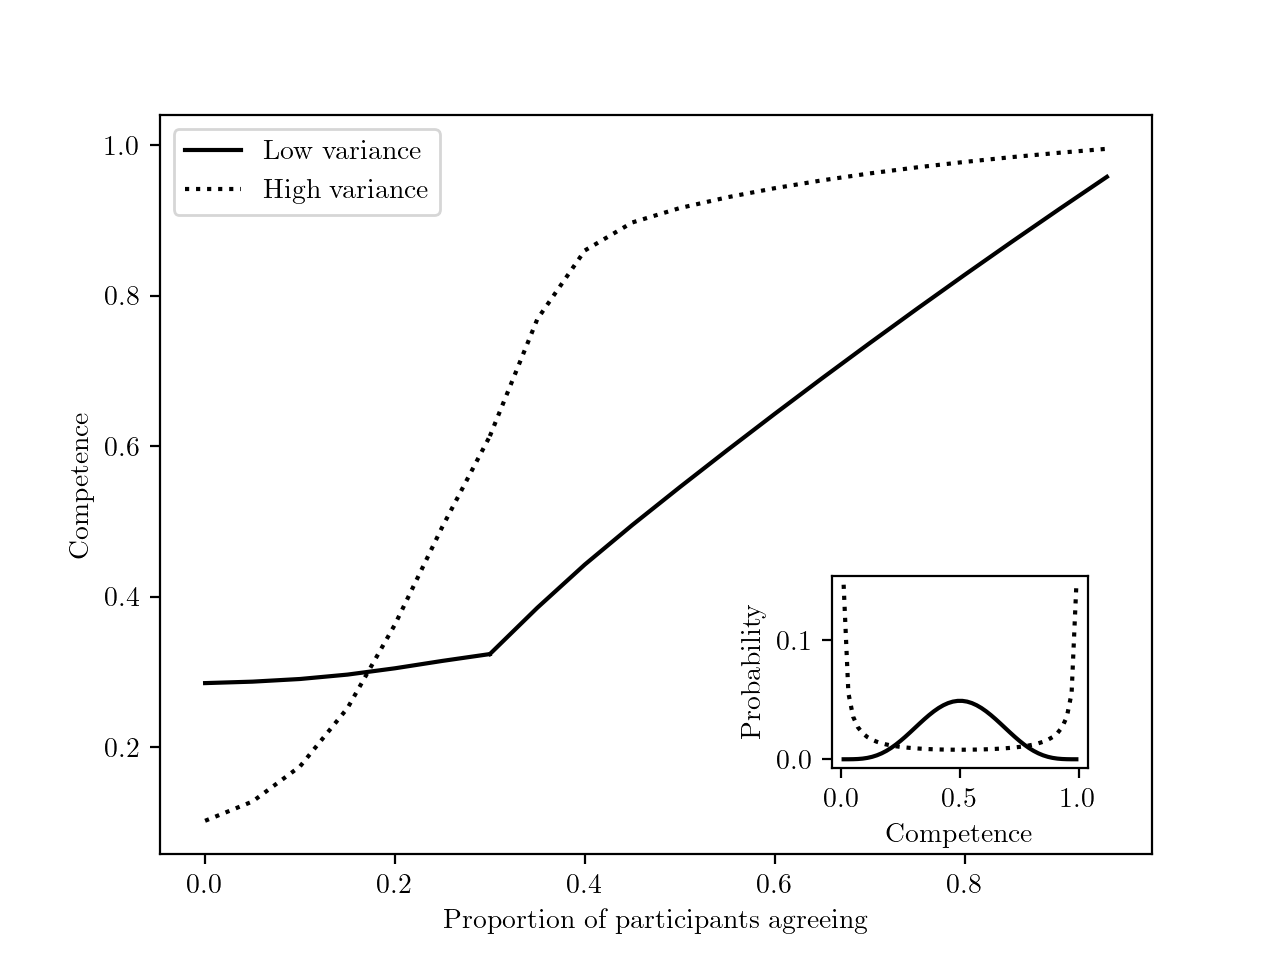
\includegraphics[width=0.75\linewidth]{figures/figure_Benoit-2} \hfill{}

\caption{Results of the analytic argument. The figure shows the average estimated competence and accuracy for a focal individual, depending on the proportion of individuals agreeing with them, in a categorical choice scenario. Here, we assume that 20 individuals answer a 5-choice question. For values higher than four, we assume that the focal individual is part of the majority. Below four, we assume that the focal individual is part of a minority, and that the majority size is four. Two situations are represented: one in which there is low variance in the distribution of competence in the population (orange line in the insert), and one in which there is high variance in this distribution (blue line in the insert).}\label{fig:figure-Benoit-2}
\end{figure}

\subsection{Simulations}\label{simulations}

In order to better understand the influence of different parameters (e.g.~degree of convergence, number of individuals) on the relationship between convergence, accuracy, and competence of informants, we conducted simulations. In all simulations, we assume agents to be unbiased and independent in their answers, but varying in their competence. All code and data regarding the simulations can be found on Open Science Framework \href{https://osf.io/6abqy/?view_only=42632bccea604fd7928dbe58e087d23b}{project page} (\url{https://osf.io/6abqy/?view_only=42632bccea604fd7928dbe58e087d23b}).

\subsubsection{Continuous case}\label{continuous-case}

Groups of agents, with each agents' competence varying, provide numerical answers. We measure how accurate these answers are, and how much they converge (i.e.~how low their variance is). We then look at the relationship between convergence and both the accuracy of the answers and the competence of the agents.

More specifically, agents provide an estimate on a scale from 1000 to 2000 (chosen to match the experiments below). Each agent is characterized by a normal distribution of possible answers. All of the agents' distributions are centered around the correct answer, but their standard deviation varies, representing varying degrees of competence. The agents' standard deviation varies from 1 (highest competence) to 1000 (lowest competence). Each agent's competence is drawn from a population competence distribution, expressed by a beta distribution, which can take different shapes. We conducted simulations with a variety of beta distributions which cover a wide range of possible competence populations (see Fig. \ref{fig:simulations} A).

A population of around 990000 agents (varying slightly as a function of group sizes) with different competence levels is generated. An answer is drawn for each agent, based on their respective competence distribution. The accuracy of this answer is defined as the squared distance to the true answer. Having a competence and an accuracy value for each agent, we randomly assign agents to groups of, e.g., three. For each group, we calculate the average of the agents' competence and accuracy. We measure the convergence of a group's answers by calculating the standard deviation of the agents' answers. We repeat this process for different sample sizes for the groups, and different competence distributions. Fig. \ref{fig:simulations} C displays the resulting relation of convergence with accuracy (left), and competence (right) for different underlying competence distributions and group sizes. We draw broad conclusions from these results after reporting the outcome of the simulations with categorical answers.

\subsubsection{Categorical case}\label{categorical-case}

In the case of categorical answers, convergence can be measured as the relative size of informants picking the same option. The Condorcet jury theorem (De Condorcet, 2014; for a recent treatment, see Dietrich \& Spiekermann, 2013) and its extensions to situations with more than two options (e.g., Hastie \& Kameda, 2005) already shows that the answer defended by the majority/plurality is more likely to be correct. Regarding competence, Romeijn and Atkinson (2011) have shown that when individuals are more competent, the share of the majority vote tends to increase. However, they have only studied a case with a uniform distribution of competence. By contrast, here, we investigate a wide range of distributions of competence, and we do not assume that all individuals are equally competent, meaning that, from an observed set of answers, we can attribute an average competence to individuals whose answers form a majority/plurality vs.~individuals whose answers form a minority.

We simulate agents whose competence varies and who have to decide between a number of options, one of which is correct. Competence is defined as a value p which corresponds to the probability of selecting the right answer (the agents then have a probability (1-p)/(m-1), with m being the number of options, of selecting any other option). Competence values range from chance level (p = 1/m) to always selecting the correct option (p = 1). Individual competence levels are drawn from the same population competence beta distributions as in the numerical case (see Fig. \ref{fig:simulations} A). Based on their competence level, we draw an answer for each agent. We measure an agent's accuracy as a binary outcome, namely whether they selected the correct option or not. In each simulation around 99900 agents (varying slightly as a function of the group size) are generated, and then randomly assigned to groups (of varying size in different simulations). Within these groups, we first calculate the share of individuals voting for each answer, allowing us to measure convergence. For example, in a scenario with three choice options and three individuals, two might vote for option A, and one for option C, resulting in two levels of convergence, \(2/3\) for A and \(1/3\) for C. For each level of convergence occurring within a group, we then compute (i) the accuracy (either 1 if the correct option or 0 else),, (ii) the average competence of agents. Across all groups, we then compute the averages of these values, for each level of convergence.

We repeat this procedure varying population competence distributions and the size of informant groups, holding the number of choice options constant at n = 3 (for simulations with varying choice options, see ESM section \ref{simulations}). Fig. \ref{fig:simulations} B shows the average accuracy (left), and the average competence (right) value as a function of convergence, across different underlying competence distributions and group sizes.

The simulations for the numerical and categorical case demonstrate a similar pattern, which can be summarized as follows:

\begin{enumerate}
\def\labelenumi{\arabic{enumi}.}
\tightlist
\item
  Irrespective of group size (and number of choice options) and of the competence distribution, there is a very strong relation between convergence and accuracy: more convergent answers tend to be more accurate.
\item
  For any group size and any competence distribution, there is a relation between convergence and the competence of the agents: more convergent answers tend to stem from more competent agents. The strength of this relation is not much affected by the number of agents whose answers are converging, but, although it is always positive, it ranges from very weak to very strong depending on the population's competence distribution.
\item
  The relation between convergence and accuracy is always much stronger than the relation between convergence and competence of the agents.
\end{enumerate}



\begin{figure}
\centering
\includegraphics{output/figures/simulations.pdf}
\caption{\label{fig:simulations}Results of the simulations. \textbf{A} Shows the different population competence distributions we considered in our simulations. In the continuous simulations, competence values of 0 correspond to a very large standard deviation (1000, with a mean of 1500, on a scale from 1000 to 2000), thereby practically taking the form of a uniform distribution, while competence of 1 corresponds to a very small standard deviation (1, on the same scale). In the categorical simulations, a competence value of 0 corresponds to chance (e.g.~in a 3-choice-options scenario, an individual picking the correct answer with a probability of \(1/3\)), while a competence value of 1 corresponds to definitely picking the correct answer. \textbf{B} Shows the results of simulations in a categorical setting with three choice options. Points represent average accuracy (left)/competence (right) values by degree of convergence (measured by the share of votes for an option), for different population competence distributions (panels) and sample sizes (colors). \textbf{C} Shows the results in a continuous setting. Regression lines represent the correlation between accuracy (left; measured by squared distance to true mean and reversed such that greater accuracy corresponds to being further up on the y-axis) or competence (right), respectively, and convergence (reversed such that greater convergence corresponds to being more right on the x-axis).}
\end{figure}

\section{Overview of the experiments}\label{overview-of-the-experiments}

Our models indicate that groups of informants are more likely to have given accurate answers, and to be competent, when their answers converge. In a series of experiments, we test whether people draw these inferences both in numerical tasks (Experiments 1, 2, 3), and in categorical tasks (Experiments 4, 5, 6). By contrast with previous studies, participants were not given any information about the tasks--how difficult they were--and the informants--how competent they might be. There has recently been much interest in investigating whether participants are able to take informational dependencies into account when evaluating convergent information (Desai, Xie, \& Hayes, 2022; Mercier \& Miton, 2019; Xie \& Hayes, 2022; Yin, Xu, Lin, Zhou, \& Guo, 2024; Yousif et al., 2019). To test whether participants took into account dependencies between the informants in the present context, this factor was manipulated in two different ways (in Experiment 2, some informants had discussed with each other; in Experiments 3 and 5, some informants had an incentive to provide the same answer). We predicted that dependencies between the informants' answers should reduce participants' reliance on the convergence of the answer as a cue to accuracy and to competence.

All experiments were preregistered. All documents, data and code can be found on Open Science Framework \href{https://osf.io/6abqy/?view_only=42632bccea604fd7928dbe58e087d23b}{project page} (\url{https://osf.io/6abqy/?view_only=42632bccea604fd7928dbe58e087d23b}). All analyses were conducted in R (version 4.2.2) using R Studio. For most statistical models, we relied on the \texttt{lme4} package and its \texttt{lmer()} function. Unless mentioned otherwise, we report unstandardized model coefficients that can be interpreted in units of the scales we use for our dependent variables.

\section{Experiment 1}\label{experiment-1}

In Experiment 1, participants were provided with a set of numerical estimates which were more or less convergent, and asked whether they thought the estimates were accurate, and whether the informants making the estimates were competent. Perceptions of accuracy were measured as the confidence in what the participants thought the correct answer was, on the basis of the numerical estimates provided: the more participants think they can confidently infer the correct answer, the more they must think the estimates accurate, on average (the results replicate with a more direct measure of accuracy, see Experiment 3). Our hypotheses were:

\textbf{\emph{H1: When making a guess based on the estimates of (independent) informants, participants will be more confident about their guess when these estimates converge compared to when they diverge.}}

\textbf{\emph{H2: Participants perceive (independent) informants whose estimates converge more as more competent than informants whose estimates diverge.}}

We had three research questions regarding the number of informants which report in the ESM (section \ref{exp1}).

\subsection{Methods}\label{methods}

\subsubsection{Participants}\label{participants}

We recruited 200 participants from the UK via Prolific (100 female, 100 male; \(age_\text{mean}\): 39.73, \(age_\text{sd}\): 15.39, \(age_\text{median}\): 35.50). Not a single participant failed our attention check. The sample size was determined on the basis of a power analysis for a t-test to detect the difference between two dependent means (``matched pairs'') run on G*Power3. The analysis suggested that a combined sample of 199 would provide us with 80\% power to detect a true effect size of Cohen's d \(\geq\) 0.2 (alpha = .05, two-tailed).

\subsubsection{Procedure}\label{procedure}

After providing their consent to participate in the study and passing an attention check, participants read the following introduction: ``Some people are playing games in which they have to estimate various quantities. Each game is different. You have no idea how competent the people are: they might be completely at chance, or be very good at the task. It's also possible that some are really good while others are really bad. Some tasks might be hard while others are easy. Across various games, we will give you the answers of several players, and ask you questions about how good they are. As it so happens, for all the games, the estimates have to be between 1000 and 2000, but all the games are completely different otherwise, and might require different skills, be of different difficulties, etc. Each player in the game makes their own estimate, completely independent of the others''. After being presented with the results of a game (Fig. \ref{fig:stimulus-exp1}), participants had to (i) make a guess about the correct answer based on the estimates they see, ``What would you guess is the correct answer, if there is one?'', (ii) estimate their confidence in this guess, ``How confident are you that your answer is at least approximately correct?'' on a 7-point Likert scale (``not confident at all'' to ``extremely confident''), (iii) estimate the competence of the group of players whose estimates they saw, ``On average, how good do you think these players are at the game?'', also on a 7-point Likert scale (from ``not good at all'' to ``extremely good'').



\begin{figure}

\includegraphics[width=1\linewidth]{output/figures/stimulus-exp1} \hfill{}

\caption{Example of two stimuli from Experiment 1, both in the 10 players condition, \textbf{A} corresponding to the convergent, \textbf{B} to the divergent condition. Similar stimuli are used in Experiments 2 and 3.}\label{fig:stimulus-exp1}
\end{figure}

\subsubsection{Design}\label{design}

We manipulated two experimental factors, with two levels each: the convergence of the estimates (how close they were to each other; levels: divergent/convergent), and the number of estimates (how many players there were; levels: three/ten). This latter factor was chiefly included to make our results more robust, and was not attached to specific hypotheses. We used a 2 (convergence: divergent/convergent) x 2 (number: three/ten) within-participant design, with each participant seeing all the conditions. Participants saw two different sets of estimates per condition, for a total of eight sets of estimates per participant.

\subsubsection{Materials}\label{materials}

We generated sets of estimates with random draws from normal distributions. First, we varied the standard deviation of these distributions to simulate the degree of convergence (150 for divergence, 20 for convergence; estimate scale ranged from 1000 to 2000). Second, we varied the number of draws (either three or ten) from these distributions. For each of the four possible resulting conditions, we generated two random draws. We repeated this process for three different sets of estimates, and participants were randomly assigned to one of these sets. More information on how the stimuli were created can be found in the ESM, section \ref{exp1}.

\subsection{Results and discussion}\label{results-and-discussion}

To account for dependencies of observations due to our within-participant design, we ran mixed models, with a random intercept and a random slopes of convergence for participants. In the models for our hypotheses, we control for the number of estimates provided to the participants (three or ten). Visualizations and descriptive statistics can be found in ESM, section \ref{exp1}. We find a positive effect of convergence on accuracy: Participants were more confident about their estimate in convergent scenarios (mean = 4.56, sd = 1.45) than in divergent ones (mean = 3.19, sd = 1.39; \(\hat{b}_{\text{Accuracy}}\) = 1.37 {[}1.225, 1.51{]}, p = \textless{} .001). We also find a positive effect of convergence on competence: participants rated players as more competent in convergent scenarios (mean = 4.75, sd = 1.24) than in divergent ones (mean = 3.52, sd = 1.27; \(\hat{b}_{\text{Competence}}\) = 1.23 {[}1.065, 1.4{]}, p = \textless{} .001).

In an exploratory, non-preregistered analysis, we tested whether the effect of convergence is larger on accuracy than on competence. To this end, we regressed the outcome score on convergence and its interaction with a binary variable indicating which outcome was asked for (accuracy or competence), while controlling for the number of informants. We do not find a statistically significant interaction that would indicate a difference of the effect of convergence (\(\hat{b}\) = 0.14 {[}-0.001, 0.271{]}, 0.052). Pooled across divergent and convergent conditions, we find that participants reported lower perceived accuracy than competence (\(\hat{b}\) = -0.26 {[}-0.359, -0.156{]}, \textless{} .001)

In summary, as predicted, when the informants' answers were more convergent, participants were more confident that their answers were correct, and they believed the informants to be more competent. This was true both when there were three informants and when there were ten informants.

\section{Experiment 2}\label{experiment-2}

We have shown that it is rational to infer that convergent estimates are more likely to be accurate, and to have been made by competent individuals, only if these individuals were independent and unbiased. However, convergence could come about differently. If the individuals do not make their estimates independently of each other, a single individual might exert a strong influence on the others, making their convergence a poor cue to their accuracy. Alternatively, all individuals might have an incentive to provide a similar, but not accurate answer. In Experiment 2, we investigate the first possibility, and the second in Experiment 3. In particular, for Experiment 2 we rely on past results showing that participants, under some circumstances, put less weight on opinions that have been formed through discussion, by contrast with more independent opinions (Harkins \& Petty, 1987; Einav, 2018; Hess \& Hagen, 2006; see also Lopes, Vala, \& Garcia-Marques, 2007). We sought to replicate this finding in the context of convergent estimates, formulating the following hypotheses:

\textbf{\emph{H1: When making a guess based on convergent estimates of informants, participants will be more confident about their guess when informants were independent compared to when they weren't (i.e.~they could discuss before).}}

\textbf{\emph{H2: Participants perceive informants whose estimates converge as more competent when they are independent, compared to when they weren't (i.e.~they could discuss before).}}

Note that these predictions only stem from past empirical results, and are not necessarily normatively justified (modeling the effects of discussion would be beyond the scope of this paper, but see Dietrich \& Spiekermann, 2024).

\subsection{Methods}\label{methods-1}

\subsubsection{Participants}\label{participants-1}

We recruited 200 participants from the UK via Prolific (100 female, 99 male, 1 not-identified; \(age_\text{mean}\): 40.54, \(age_\text{sd}\): 13.56, \(age_\text{median}\): 38.50). Not a single participant failed our attention check. As for experiment 1, the sample size was determined on the basis of a power analysis for a t-test to detect the difference between two dependent means (``matched pairs'') run on G*Power3. The analysis suggested that a combined sample of 199 would provide us with 80\% power to detect a true effect size of Cohen's d \(\geq\) 0.2 (alpha = .05, two-tailed).

\subsubsection{Design}\label{design-1}

In a within-participants design, participants saw both an independence condition, in which they were told ``Players are asked to make completely independent decisions -- they cannot see each other's estimates, or talk with each other before giving their estimates,'' and a dependence condition, in which they were told ``Players are asked to talk with each other about the game at length before giving their estimates.''

\subsubsection{Materials}\label{materials-1}

We used the materials generated for the convergent condition of Experiment 1. By contrast to Experiment 1, participants saw only two stimuli in total (one set of estimates per condition), and we only used stimuli involving groups of three informants. Otherwise, we proceeded just as in Experiment 1: we randomly assigned individual participants to one of the three series of stimuli, and for each participant, we randomized the order of appearance of conditions.

\subsection{Results and discussion}\label{results-and-discussion-1}

To account for dependencies of observations due to our within-participant design, we ran mixed models, with a random intercept for participants. Visualizations and descriptive statistics can be found in ESM, section \ref{exp2}. The data does not support our hypotheses. Participants were slightly less confident about their estimates when the converging informants were independent (mean = 3.78, sd = 1.50), compared to when they discussed (mean = 4.03, sd = 1.39; \(\hat{b}_{\text{Accuracy}}\) = -0.26 {[}-0.462, -0.048{]}, p = 0.016). The effect is small, but in the opposite direction of what we had predicted. We do not find an effect regarding competence (\(\hat{b}_{\text{Competence}}\) = -0.12 {[}-0.272, 0.032{]}, p = 0.120).

Contrary to the hypotheses, participants did not deem convergent estimates made after a discussion, compared to independently made estimates, to be less accurate, or produced by less competent individuals. This might stem from the fact that participants, in various situations, neglect informational dependencies (Yousif et al., 2019), or from the fact that discussing groups actually perform better than non-discussing groups in a range of tasks (for review, see, e.g., Mercier, 2016), including numerical estimates (e.g. Mercier \& Claidière, 2022). As a result, the participants in the current experiment might have been behaving rationally when they did not discount the estimates made after discussion.

\section{Experiment 3}\label{experiment-3}

Experiment 3 tests whether participants are sensitive to another potential source of dependency between convergent estimates: when the individuals making the estimate share an incentive to bias their estimates and disregard accuracy. Even though Experiment 3 is formally similar to Experiment 1, the setting is different, as participants were told that they would be looking at (fictional) predictions of experts for stock values, instead of the answers of individuals in abstract games. In the conflict of interest condition, the experts had an incentive to value the stock in a given way, while they had no such conflict of interest in the independence condition. We tested for an interaction, namely whether the positive effect of convergence is reduced when informants are systematically biased, compared to when they are not. On this basis, we formulate four hypotheses, two of which are identical to those of Experiment 1, and only apply in the independent condition, and two that bear on the interaction:

\textbf{\emph{H1a: Participants perceive predictions of independent informants as more accurate when they converge compared to when they diverge.}}

\textbf{\emph{H1b: Participants perceive independent informants as more competent when their predictions converge compared to when they diverge.}}

\textbf{\emph{H2a: The effect of convergence on accuracy (H1a) is more positive in a context where informants are independent compared to when they are in a conflict of interest.}}

\textbf{\emph{H2b: The effect of convergence on competence (H1b) is more positive in a context where informants are independent compared to when they are in a conflict of interest.}}

We have not conducted simulations to validate these predictions. However, given the operationalization chosen, in which convergence should provide little evidence of either accuracy or competence, we believe the predictions regarding the superiority of the independent informants stem naturally from the model of independent informants presented above.

\subsection{Methods}\label{methods-2}

\subsubsection{Participants}\label{participants-2}

The interaction design of our third experiment made the power analysis more complex and less standard than for experiments one and two. Because we could build upon data from the first experiment, we ran a power analysis by simulation. The simulation code is available on the OSF, and the procedure is described in the preregistration document. The simulation suggested that 100 participants provide a significant interaction term between 95\% and 97\% of the time, given an alpha threshold for significance of 0.05. Due to uncertainty about our effect size assumptions and because we had resources for a larger sample, we recruited 199 participants for this study -- again, from the UK and via Prolific (99 female, 100 male; \(age_\text{mean}\): 40.30, \(age_\text{sd}\): 12.72, \(age_\text{median}\): 38).

\subsubsection{Procedure}\label{procedure-1}

After providing their consent to participate in the study and passing an attention check, participants read the following introduction: ``You will see four scenarios in which several experts predict the future value of a stock. You have no idea how competent the experts are. It's also possible that some are really good while others are really bad. As it so happens, in all scenarios, the predictions for the value of the stock have to lie between 1000 and 2000. Other than that, the scenarios are completely unrelated: it is different experts predicting the values of different stocks every time.'' Participants then saw the four scenarios, each introduced by a text according to the condition the participant was assigned to. To remove any potential ambiguity about participants' inferences on the accuracy of the estimates, we replaced the question about confidence to one bearing directly on accuracy: ``On average, how accurate do you think these three predictions are?'' on a 7-point Likert scale (``not accurate at all'' to ``extremely accurate''). The question about competence read: ``On average, how good do you think these three experts are at predicting the value of stocks?'', also assessed on a 7-point Likert scale (from ``not good at all'' to ``extremely good'').

\subsubsection{Design}\label{design-2}

We manipulated two factors: informational dependency (two levels, independence and conflict of interest; between participants) and convergence (two levels, convergence and divergence; within participants). In the independence condition, the participants read ``Experts are independent of each other, and have no conflict of interest in predicting the stock value - they do not personally profit in any way from any future valuation of the stock.'' In the conflict of interest condition, the participants read ``All three experts have invested in the specific stock whose value they are predicting, and they benefit if other people believe that the stock will be valued at {[}mean of respective distribution{]} in the future.''

\subsubsection{Materials}\label{materials-2}

The distributions presented were similar to those of Experiment 1, although generated in a slightly different manner (see ESM, section \ref{exp3}). Each participant rated four scenarios, two for each level of convergence. By contrast to Experiment 1, all scenarios only involved groups of three informants.

\subsection{Results and discussion}\label{results-and-discussion-2}

To account for dependencies of observations due to our within-participant design, we ran mixed models, with a random intercept and a random slope for convergence for participants. We find evidence for all four hypotheses. As for the first set of hypotheses, to match the setting of experiment one, we reduced the sample of Experiment 3 to half of the participants, namely those who were assigned to the independence condition. On this reduced sample, we ran the exact same analyses as in Experiment 1 and replicated the results. As for accuracy, participants rated informants in convergent scenarios (mean = 5.28, sd = 1.05) as more accurate than in divergent ones (mean = 3.40, sd = 1.08; \(\hat{b}_{\text{Accuracy}}\) = 1.88 {[}1.658, 2.102{]}, p = \textless{} .001). As for competence, participants rated informants in convergent scenarios (mean = 5.24, sd = 0.99) as more competent than in divergent ones (mean = 3.61, sd = 1.11; \(\hat{b}_{\text{Competence}}\) = 1.62 {[}1.411, 1.839{]}, p = \textless{} .001).

The second set of hypotheses targeted the interaction of informational dependency and convergence (Fig. \ref{fig:exp3-plot}). In the independence condition, the effect of convergence on accuracy was more positive (\(\hat{b}_{\text{interaction, Accuracy}}\) = 0.99 {[}0.634, 1.348{]}, p = \textless{} .001) than in the conflict of interest condition (\(\hat{b}_{\text{baseline}}\) = 0.89 {[}0.636, 1.142{]}, p = \textless{} .001). Likewise the effect of convergence on competence is more positive (\(\hat{b}_{\text{interaction, Competence}}\) = 0.80 {[}0.474, 1.13{]}, p = \textless{} .001) than in the conflict of interest condition (\(\hat{b}_{\text{baseline}}\) = 0.82 {[}0.591, 1.056{]}, p = \textless{} .001).



\begin{figure}
\centering
\includegraphics{output/figures/exp3-plot.pdf}
\caption{\label{fig:exp3-plot}Results of Experiment 3, showing the distributions of accuracy and competence ratings by convergence and informational dependency.}
\end{figure}

In an exploratory, non-preregistered analysis, we tested whether the effect of convergence is larger on accuracy than on competence. To this end, we regressed the outcome score on convergence and its interaction with a binary variable indicating which outcome was asked for (accuracy or competence), while controlling for informational dependency. We find a negative interaction effect, indicating that pooled across independent and conflict of interest conditions, the effect of convergence had as smaller effect on competence than on accuracy (\(\hat{b}\) = -0.16 {[}-0.294, -0.028{]}, 0.018). Pooled across all conditions, participants reported higher perceived competence than accuracy (\(\hat{b}\) = 0.11 {[}0.025, 0.191{]}, 0.011).

Experiment 3 shows that, when the individuals making the estimates are systematically biased, participants put less weight on the convergence of their estimates to infer that the estimates are accurate, and that the individuals making them are competent.

\section{Experiment 4}\label{experiment-4}

In a second series of experiments, we test similar predictions to those of the previous experiments, but in a categorical choice context. The set-up is similar to that of Experiment 1, except that the outcomes seen by the participants are not numerical estimates, but choices made between a few options. An additional difference is that participants rate a focal informant, and not a group of informants. There were two reasons for this choice: First, accuracy is not on a continuum as in the first three experiments (an option was either correct or not), so forming an average across informants who chose different options was less sensible. Second, rating a focal individual allowed us to have a minority condition, which would not have been possible when providing an average rating for a group. Experiment 4 tests hypotheses that are analogous to those of Experiment 1:

\textbf{\emph{H1: Participants perceive an estimate of an independent informant as more accurate the more it converges with the estimates of other informants.}}

\textbf{\emph{H2: Participants perceive an independent informant as more competent the more their estimate converges with the estimates of other informants.}}

\subsection{Methods}\label{methods-3}

\subsubsection{Participants}\label{participants-3}

We ran a power simulation to inform our choice of sample size. All assumptions and details on the procedure can be found on the OSF. We ran two different power analyses, one for each outcome variable. We set the power threshold for our experiment to 90\%. The power simulation for accuracy suggested that even for as few as 10 participants (the minimum sample size we simulated data for), we would have a power of close to 100\%. The simulation for competence suggested that we achieve statistical power of at least 90\% with a sample size of 30. Due to uncertainty about our assumptions and because it was within our budget, we recruited 100 participants, from the UK and via Prolific (50 female, 50; \(age_\text{mean}\): 37.32, \(age_\text{sd}\): 11.53, \(age_\text{median}\): 36).

\subsubsection{Procedure}\label{procedure-2}

After providing their consent to participate in the study and passing an attention check, participants read the following introduction: ``To be able to understand the task, please read the following instructions carefully: Some people are playing games in which they have to select the correct answer among three answers. You will see the results of several of these games. Each game is different, with different solutions and involving different players. All players answer independently of each other. At first, you have no idea how competent each individual player is: they might be completely at chance, or be very good at the task. It's also possible that some players are really good while others are really bad. Some games might be difficult while others are easy. Your task will be to evaluate the performance of one of the players based on what everyone's answers are.'' They were then presented to the results of eight such games (Fig. \ref{fig:stimulus-exp4}). To assess perceived accuracy, we asked: ``What do you think is the probability of player 1 being correct?''. Participants answered with a slider on a scale from 0 to 100. To assess perceived competence, we asked participants: ``How competent do you think player 1 is in games like these?'' Participants answered on a 7-point Likert scale (from (1)``not competent at all'' to (2)``extremely competent'').



\begin{figure}
\centering
\includegraphics{output/figures/stimulus-exp4.pdf}
\caption{\label{fig:stimulus-exp4}One set of stimuli by level of convergence, in Experiment 4 (similar stimuli are used in Experiments 5 and 6). A full set of stimuli can be found in the ESM, section \ref{exp4}.}
\end{figure}

\subsubsection{Design}\label{design-3}

We manipulated convergence within participants, by varying the ratio of players choosing the same response as a focal player (i.e.~the one that participants evaluate). The levels of convergence are: (i) consensus, where all three players pick the same option {[}coded value = 3{]}; (ii) majority, where either the third or second player picks the same option as the first player {[}coded value = 2{]}; (iii) dissensus, where all three players pick different options {[}coded value = 1{]}; (iv) minority, where the second and third player pick the same option, but one that is different from the first player's choice {[}coded value = 0{]}. In our analysis, we treat convergence as a continuous variable, assigning the coded values in squared parenthesis here.

\subsubsection{Materials}\label{materials-3}

All participants saw all four conditions, with two stimuli per condition. Each participant therefore saw eight stimuli in total (4 convergence levels x 2 stimuli).

\subsection{Results and discussion}\label{results-and-discussion-3}

To account for dependencies of observations due to our within-participant design, we ran mixed models, with a random intercept and a random slope for participants.

As in the numerical setting, we found a positive effect of convergence on both accuracy (\(\hat{b}_{\text{Accuracy}}\) = 16.84 {[}15.009, 18.668{]}, p = \textless{} .001; on a scale from 0 to 100) and competence (\(\hat{b}_{\text{Competence}}\) = 0.68 {[}0.578, 0.788{]}, p = \textless{} .001; on a scale from 1 to 7).

In the ESM (section \ref{exp4}), we show that compared to what the normative models would predict, participants underestimate the effect of convergence on both accuracy and competence, but especially on accuracy.

In an exploratory, non-preregistered analysis, we tested whether the effect of convergence is larger on accuracy than on competence. To do so, we first standardized both outcome scores to account for the different scales. We then regressed the outcome score on convergence and its interaction with a binary variable indicating which outcome was asked for (accuracy or competence). We find a negative interaction, indicating that convergence had a smaller effect on competence than on accuracy (\(\hat{b}\) = -0.10 {[}-0.136, -0.053{]}, \textless{} .001; units in standard deviations).

\section{Experiment 5}\label{experiment-5}

Experiment 5 is a conceptual replication of Experiment 3 in a categorical instead of a numerical case: are participants less likely to infer that more convergent estimates are more accurate, and the individuals who made them more competent, when the estimates are made by individuals with a conflict of interest pushing them to all provide a given answer, compared to when they are made by independent individuals? The independence condition of Experiment 5 also serves as a replication of Experiment 4, leading to the following hypotheses:

\textbf{\emph{H1a: Participants perceive an estimate of an independent informant as more accurate the more it converges with the estimates of other informants.}}

\textbf{\emph{H1b: Participants perceive an independent informant as more competent the more their estimate converges with the estimates of other informants.}}

\textbf{\emph{H2a: The effect of convergence on accuracy (H1a) is more positive in a context where informants are independent compared to when they are biased (i.e.~share a conflict of interest to pick a given answer).}}

\textbf{\emph{H2b: The effect of convergence on competence (H1b) is more positive in a context where informants are independent compared to when they are biased (i.e.~share a conflict of interest to pick a given answer).}}

\subsection{Methods}\label{methods-4}

\subsubsection{Participants}\label{participants-4}

We ran a power simulation to inform our choice of sample size. All assumptions and details on the procedure can be found on the OSF. We ran two different power analyses, one for each outcome variable. We set the power threshold for both to 90\%.

The power simulation for accuracy suggested that for 80 participants, we would have a power of at least 90\% for the interaction effect. The simulation for competence suggested that with already 40 participants, we would detect an interaction, but only with 60 participants would we also detect an effect of convergence. Due to uncertainty about our assumptions and because resources were available for a larger sample, we recruited 200 participants, in the UK and via Prolific (99 female, 100, 1 non-identified; \(age_\text{mean}\): 41.88, \(age_\text{sd}\): 13.94, \(age_\text{median}\): 39).

\subsubsection{Procedure}\label{procedure-3}

After providing their consent to participate in the study and passing an attention check, participants read the following introduction: ``We will show you three financial advisors who are giving recommendations on investment decisions. They can choose between three investment options. Their task is to recommend one. You will see several such situations. They are completely unrelated: it is different advisors evaluating different investments every time. At first you have no idea how competent the advisors are: they might be completely at chance, or be very good at the task. It's also possible that some are really good while others are really bad. Some tasks might be difficult while others are easy. Your task will be to evaluate the performance of one of the advisors based on what everyone's answers are.'' To assess perceptions of accuracy, we asked: ``What do you think is the probability of advisor 1 making the best investment recommendation?''. Participants answered with a slider on a scale from 0 to 100. To assess perceptions of competence, we asked: ``How competent do you think advisor 1 is regarding such investment recommendations?'' Participants answered on a 7-point Likert scale (from (1)``not competent at all'' to (7)``extremely competent'').

\subsubsection{Design}\label{design-4}

We manipulated convergence within participants, and conflict of interest between participants. In the conflict of interest condition, experts were introduced this way: ``The three advisors have already invested in one of the three options, the same option for all three. As a result, they have an incentive to push that option in their recommendations.'' Participants assigned to the independence condition read: ``The three advisors are independent of each other, and have no conflict of interest in making investment recommendations.''

\subsubsection{Materials}\label{materials-4}

We used the same stimuli as in Experiment 4. Identical to Experiment 4, participants saw all four convergence conditions, with two stimuli (i.e.~expert predictions) per condition. Each participant therefore saw eight stimuli in total (4 convergence levels x 2 stimuli).

\subsection{Results and discussion}\label{results-and-discussion-4}

To account for dependencies of observations due to our within-participant design, we ran mixed models, with a random intercept and a random slope for convergence for participants.

We find evidence for all four hypotheses (see Fig. \ref{fig:exp5-plot}). To test H1a and H1b, we use the same analyses as in Experiment 4, restricted on the independence condition, and replicate the results. We find a positive effect of convergence on both accuracy (\(\hat{b}_{\text{Accuracy}}\) = 12.34 {[}10.362, 14.311{]}, p = \textless{} .001) and competence (\(\hat{b}_{\text{Competence}}\) = 0.56 {[}0.459, 0.665{]}, p = \textless{} .001).

The second set of hypotheses targeted the interaction of informational dependency and convergence (Fig. \ref{fig:exp5-plot}). In the independence condition, the effect of convergence on accuracy was more positive (\(\hat{b}_{\text{interaction, Accuracy}}\) = 3.01 {[}0.027, 5.988{]}, p = 0.048) than in the conflict of interest condition (\(\hat{b}_{\text{baseline}}\) 9.33 {[}7.232, 11.426{]}, p = \textless{} .001). Likewise, the effect of convergence on competence was more positive (\(\hat{b}_{\text{interaction, Competence}}\) = 0.16 {[}0.014, 0.316{]}, p = 0.032) than in the conflict of interest condition (\(\hat{b}_{\text{baseline}}\) = 0.40 {[}0.291, 0.503{]}, p = \textless{} .001).



\begin{figure}
\centering
\includegraphics{output/figures/exp5-plot.pdf}
\caption{\label{fig:exp5-plot}Interaction of convergence and informational dependency.}
\end{figure}

In an exploratory, non-preregistered analysis, we tested whether the effect of convergence is larger on accuracy than on competence. To do so, we first standardized both outcome scores to account for the different scales. We then regressed the outcome score on convergence and its interaction with a binary variable indicating which outcome was asked for (accuracy or competence), while controlling for informational dependency. We find a negative interaction, indicating that convergence had a smaller effect on competence than on accuracy (\(\hat{b}\) = -0.08 {[}-0.113, -0.044{]}, \textless{} .001; units in standard deviations).

\section{Experiment 6}\label{experiment-6}

Experiment 6 is a replication and extension of Experiment 4 in which we test the effect of the number of choice options (three and ten, instead of only three). Our simulations suggested that, at least for some underlying population competence distributions, consensus should be more indicative of competence when there are more choice options, compared to fewer (see ESM, section \ref{simulations} and \ref{exp6}).

First, considering only the three options condition, we ran a direct replication of experiment 4. Second, following the results from our model, we predict that

\textbf{\emph{H1: The effect of convergence on accuracy (H1a) is more positive in a context when informants can choose among ten response options compared to when they can choose among only three.}}

\textbf{\emph{H2: The effect of convergence on competence (H1b) is more positive in a context when informants can choose among ten response options compared to when they can choose among only three.}}

\subsection{Methods}\label{methods-5}

\subsubsection{Participants}\label{participants-5}

We ran a power simulation to inform our choice of sample size. All assumptions and details on the procedure can be found on the OSF. We used previous experiments and estimates of our models to inform our choice of parameter values. We ran two different power analyses, one for each outcome variable. We set the power threshold for our experiment to 90\%. The power simulation for accuracy suggested that for 140 participants we would cross the power threshold of 90\% for the interaction effect (power = 0.928). The simulation for competence suggested that with 300 participants, we would detect an interaction with a power of 87\%. Due to budget constraints, we considered aiming for a sample of 300 participants as good enough, although slightly below our threshold. Due to two failed attention checks, our final sample consisted of 298 subjects, recruited, as in all experiments, in the UK and via Prolific (149 female, 149, 1 non-identified; \(age_\text{mean}\): 42.09, \(age_\text{sd}\): 13.06, \(age_\text{median}\): 40).

\subsubsection{Procedure}\label{procedure-4}

We used the same procedure as in Experiment 4, with the addition of one condition described below.

\subsubsection{Design}\label{design-5}

The number of choice options was manipulated between participants. Participants were randomly assigned to either see stimuli with three options (as in Experiment 4), or stimuli with ten options. Participants assigned to the ten options condition were divided into one of two distinct sub-conditions: one in which the range of the answers corresponds to the range of the three options condition, and another with increased range (see ESM, section \ref{exp6}). We found no differences between the two sub-conditions and collapsed them into a single ten options condition.

\subsubsection{Materials}\label{materials-5}

For the three options condition, we used the same stimuli as in Experiments 4 and 5. For the ten options condition, we created new sets of stimuli (see ESM, section \ref{exp6}). Identical to Experiments 4 and 5, participants saw all four convergence conditions, with two stimuli per condition. Each participant therefore saw eight stimuli in total.

\subsection{Results and discussion}\label{results-and-discussion-5}

To account for dependencies of observations due to our within-participant design, we ran mixed models, with a random intercept and a random slope for convergence for participants.

We replicate the results of experiment 4, but do not find evidence for an interaction between convergence and the number of choice options. To match the setting of experiment one, we reduced the sample to half of the participants, namely those who were assigned to the three options condition. On this reduced sample, we ran the exact same analyses as in experiment 4 and replicated the results. We find a positive effect of convergence on both accuracy (\(\hat{b}_{\text{Accuracy}}\) = 15.68 {[}14.112, 17.246{]}, p = \textless{} .001) and competence (\(\hat{b}_{\text{Competence}}\) = 0.65 {[}0.564, 0.736{]}, p = \textless{} .001). This finding also holds across the entire sample, pooling three and ten choice option observations (\(\hat{b}_{\text{Accuracy}}\) = 16.30 {[}15.124, 17.485{]}, \textless{} .001; \(\hat{b}_{\text{Competence}}\) = 0.68 {[}0.611, 0.739{]}, \textless{} .001).

We do not find evidence of an interaction, i.e.~evidence that the number of choice options changes the effect of convergence (\(\hat{b}_{\text{interaction, Accuracy}}\) = 1.25 {[}-1.11, 3.613{]}, 0.298; \(\hat{b}_{\text{interaction, Competence}}\) = 0.05 {[}-0.078, 0.178{]}, 0.442).

We tested whether the effect of convergence is larger on accuracy than on competence in an exploratory, non-preregistered analysis. To this end, we first standardized both outcome scores to account for the different scales. We then regressed the outcome score on convergence and its interaction with a binary variable indicating which outcome was asked for (accuracy or competence), while controlling for the number of choice options. In line with all previous experiments, we find a negative interaction, indicating that convergence had a smaller effect on competence than on accuracy (\(\hat{b}\) = -0.05 {[}-0.075, -0.023{]}, \textless{} .001).

Experiment 6 replicates Experiments 3 and 4 (independence condition), but suggests that the number of options the informants choose from does not powerfully affect participants' estimates of the informants' accuracy or competence. In the ESM, section \ref{exp6}, we show that, compared to our model, participants underestimate the effect of the number of choice options.

\section{General discussion}\label{general-discussion}

Using both analytical arguments and simulations, we have shown that, under a wide range of parameters, more convergent answers tend to be more accurate, and to have been made by more competent informants.

In two experiments (Experiment 1, and independence condition of Experiment 3), we find that participants presented with a set of more (rather than less) convergent numerical estimates find the estimates more accurate, and the individuals making the estimates more competent, thus drawing normatively justified inferences. Experiment 2 suggests that participants do not think that a discussion between the individuals makes their convergence less indicative of accuracy or their competence. By contrast, Experiment 3 reveals that, when the individuals making the estimates are systematically biased by a conflict of interest, participants put less weight on the convergence of their estimates.

Similar results are obtained in a categorical choice context, in which participants see the answers of individuals made within a limited set of options. Experiments 4, 5 (independence condition), and 6 show that, the more the answers converge, the more participants believe them to be accurate and the individuals who made to be competent, again drawing normatively justified inferences. Experiment 5 shows that these inferences are weakened when the convergence can be explained by a conflict of interest (as in Experiment 3). Experiment 6 fails to find an effect of the number of options.

We also observe that, in line with our simulations, participants draw stronger inferences from convergence to accuracy than to competence in five of the six experiments.

On the whole, participants thus appear to draw normatively justified inferences: 1. They infer that more convergent answers are more accurate; 2. They infer that more convergent answers are coming from more competent informants; 3. The inference on accuracy tends to be stronger than the inference on competence ; 4. Both the inference on accuracy and on the inference on competence are weaker when the informants have a conflict of interest, but not when they are merely discussing with each other. The only exception appears to be that participants do not take into account the number of options in categorical choices scenarios.

\section{Conclusion}\label{conclusion}

When people see that others agree with each other, they tend to believe that they are right. This inference has been evidenced in several experiments, both for numerical estimates (Budescu \& Rantilla, 2000; Budescu et al., 2003; Budescu \& Yu, 2007; e.g. Molleman et al., 2020; Yaniv et al., 2009), and for categorical choices (e.g., Morgan et al., 2012; for review, see Mercier \& Morin, 2019). However, these experiments do not test whether this inference of accuracy of the information extends to an inference of competence of the informants. Moreover, by their design, participants arguably assumed a degree of competence among the informants. For instance, when children are confronted with several individuals who agree on how to name a novel object (e.g. Corriveau et al., 2009), they can assume that these (adult) individuals tend to know what the names of objects are. If a certain competence of the informants is assumed, then well-known results from the literature on judgment aggregation--the wisdom of crowds--show that the average opinion of a set of individuals is, in a wide range of circumstances, more likely to be accurate than that of a single individual (e.g. Larrick \& Soll, 2006).

Here, we assumed no prior knowledge of individual competence, asking the question: if we see informants, whose competence is unknown, converge on an answer, is it rational to infer that this answer is more likely to be correct, and that the informants are likely to be competent? We have shown that the answer is yes on both counts--assuming there is no systematic bias among the informants. An analytical argument and a series of simulations revealed that, for both the numerical choice context and the categorical choice context, the more individuals agree on an answer, the more likely the answer is correct, and the more likely the individuals are competent, with the former effect being stronger than the latter. Moreover, this is true for a wide range of assumed population distributions of competence. In a series of experiments, we have shown that participants (UK) draw these inferences, but that they do so less when there is reason to assume a bias among informants.

The results--both simulations and experiments--are a novel contribution to the wisdom of crowds literature. In this literature--in particular that relying on the Condorcet Jury Theorem--a degree of competence is assumed in the individuals providing some answers. From that competence, it can be inferred that the individuals will tend to agree, and that their answers will tend to be accurate. Here, we have shown that the reverse inference--from agreement to competence--is also warranted, and that it is warranted under a wide range of circumstances: If one does not suspect any systematic bias, convergence alone can be a valid cue when determining who tends to be an expert. This finding qualifies work suggesting that people need a certain degree of expertise themselves, in order to figure out who is an expert (Hahn, Merdes, \& Sydow, 2018; Nguyen, 2020).

The present experiments show that people draw inferences from convergence to accuracy and to competence, but then do not precisely show how they do it. As suggested in the introduction, it is plausible that participants use the combination of two heuristics: one leading them from convergence to accuracy, and one from accuracy to competence. This two step process is coherent with the observation that the inference from convergence to accuracy (one step) is stronger than that from convergence to competence (two steps). However, our results are also compatible with participants performing two inferences from convergence, one to accuracy and one to competence, the latter being weaker because the inferences roughly follow the normative model. Our results are coherent with work on other mechanisms of epistemic vigilance that process the combination of several informants' opinions, showing that these mechanisms rely on sensible cues, but also systematically fail to take some subtle cues into account (Mercier \& Morin, 2019).

A most prominent context in which the inferences uncovered here might play a role is that of science. Much of science is counterintuitive, and most people do not have the background knowledge to evaluate most scientific evidence. However, science is, arguably, the institution in which individuals end up converging the most in their opinions (on consensus being the defining trait of science by contrast with other intellectual enterprises, see Collins, 2002). For instance, scientists within many disciplines agree on things ranging from the distance between the solar system and the center of the galaxy to the atomic structure of DNA. This represents an incredible degree of convergence. When people hear that scientists have measured the distance between the solar system and the center of the galaxy, if they assume that there is a broad agreement within the relevant experts, this should lead them to infer that this measure is accurate, and that the scientists who made it are competent. Experiments have already shown that increasing the degree of perceived consensus among scientists tends to increase acceptance of the consensual belief (Van Stekelenburg, Schaap, Veling, Van 'T Riet, \& Buijzen, 2022), but it hasn't been shown yet that the degree of consensus also affects the perceived competence of scientists.

In the case of science, the relationship between convergence and accuracy is broadly justified. However, at some points of history, there has been broad agreement on misbeliefs, such as when Christian theologians had calculated that the Earth was approximately six thousand years old. To the extent that people were aware of this broad agreement, and believed the theologians to have reached it independently of each other, this might have not only fostered acceptance of this estimate of the age of the Earth, but also a perception of the theologians as competent.

The current study has a number of limitations. In our simulations, we assume agents to be independent and unbiased. Following previous work generalizing the Condorcet Jury Theorem to cases of informational dependency (Ladha, 1992), more robust simulations would show that--while still assuming no systematic bias--our results hold even when agents influence each others' answers. Regarding our experiments, if the very abstract materials allow us to remove most of the priors that participants might have, they might also reduce the ecological validity of the results. Although the main results replicate well across our experiments, and we can thus be reasonably certain of their robustness, it's not clear how much they can be generalized. Experimental results with convenience samples can usually be generalized at least to the broader population the samples were drawn from--here, UK citizens (Coppock, 2019). However, we do not know whether they would generalize to other cultures.

These limitations could be overcome by replicating the present results in different cultures, using more ecologically valid stimuli. For instance, it would be interesting to test whether the inference described here, from convergence to competence, might be partly responsible for the fact that people tend to believe scientists to be competent (Cologna et al., 2024). Finally, future studies could also attempt to systematically model cases of informational dependencies more subtle than those used in Experiments 3 and 5, to derive and test normative predictions.

\subsubsection{Data availability}\label{data-availability}

Data for all experiments and the simulations is available on the OSF project page (\url{https://osf.io/6abqy/?view_only=42632bccea604fd7928dbe58e087d23b}).

\subsubsection{Code availability}\label{code-availability}

The code used to create all results (including tables and figures) of this manuscript is also available on the OSF project page (\url{https://osf.io/6abqy/?view_only=42632bccea604fd7928dbe58e087d23b}).

\subsubsection{Competing interest}\label{competing-interest}

The authors declare having no competing interests.

\FloatBarrier

\section{References}\label{references}

\phantomsection\label{refs}
\begin{CSLReferences}{1}{0}
\bibitem[\citeproctext]{ref-aschStudiesIndependenceConformity1956}
Asch, S. E. (1956). Studies of independence and conformity: I. A minority of one against a unanimous majority. \emph{Psychological Monographs: General and Applied}, \emph{70}(9), 1--70. \url{https://doi.org/10.1037/h0093718}

\bibitem[\citeproctext]{ref-bednarikEffectivenessImperfectWeighting2015a}
Bednarik, P., \& Schultze, T. (2015). The effectiveness of imperfect weighting in advice taking. \emph{Judgment and Decision Making}, \emph{10}(3), 265--276. \url{https://doi.org/10.1017/S1930297500004666}

\bibitem[\citeproctext]{ref-bernardChildrenWeighNumber2015a}
Bernard, S., Harris, P., Terrier, N., \& Clément, F. (2015). Children weigh the number of informants and perceptual uncertainty when identifying objects. \emph{Journal of Experimental Child Psychology}, \emph{136}, 70--81. \url{https://doi.org/10.1016/j.jecp.2015.03.009}

\bibitem[\citeproctext]{ref-bernardFourSixYearOldChildren2015}
Bernard, S., Proust, J., \& Clément, F. (2015). Four- to Six-Year-Old Children's Sensitivity to Reliability Versus Consensus in the Endorsement of Object Labels. \emph{Child Development}, \emph{86}(4), 1112--1124. \url{https://doi.org/10.1111/cdev.12366}

\bibitem[\citeproctext]{ref-budescuConfidenceAggregationExpert2000}
Budescu, D. V., \& Rantilla, A. K. (2000). Confidence in aggregation of expert opinions. \emph{Acta Psychologica}, \emph{104}(3), 371--398. \url{https://doi.org/10.1016/S0001-6918(00)00037-8}

\bibitem[\citeproctext]{ref-budescuEffectsAsymmetryAdvisors2003}
Budescu, D. V., Rantilla, A. K., Yu, H.-T., \& Karelitz, T. M. (2003). The effects of asymmetry among advisors on the aggregation of their opinions. \emph{Organizational Behavior and Human Decision Processes}, \emph{90}(1), 178--194. \url{https://doi.org/10.1016/S0749-5978(02)00516-2}

\bibitem[\citeproctext]{ref-budescuAggregationOpinionsBased2007}
Budescu, D. V., \& Yu, H.-T. (2007). Aggregation of opinions based on correlated cues and advisors. \emph{Journal of Behavioral Decision Making}, \emph{20}(2), 153--177. \url{https://doi.org/10.1002/bdm.547}

\bibitem[\citeproctext]{ref-chenChildrenTrustConsensus2013}
Chen, E. E., Corriveau, K. H., \& Harris, P. L. (2013). Children Trust a Consensus Composed of Outgroup Members-But Do Not Retain That Trust. \emph{Child Development}, \emph{84}(1), 269--282. \url{https://doi.org/10.1111/j.1467-8624.2012.01850.x}

\bibitem[\citeproctext]{ref-collinsSociologyPhilosophiesGlobal2002}
Collins, R. (2002). \emph{The sociology of philosophies: a global theory of intellectual change} (4. print., 1. Harvard Univ. Pr. paperback ed., 2000). Cambridge, Mass. London: Belknap Press of Harvard Univ. Press.

\bibitem[\citeproctext]{ref-colognaTrustScientistsTheir2024}
Cologna, V., Mede, N. G., Berger, S., Besley, J., Brick, C., Joubert, M., \ldots{} Linden, D. S. van der. (2024). \emph{Trust in scientists and their role in society across 67 countries}. \url{https://doi.org/10.31219/osf.io/6ay7s}

\bibitem[\citeproctext]{ref-coppockGeneralizingSurveyExperiments2019}
Coppock, A. (2019). Generalizing from Survey Experiments Conducted on Mechanical Turk: A Replication Approach. \emph{Political Science Research and Methods}, \emph{7}(3), 613--628. \url{https://doi.org/10.1017/psrm.2018.10}

\bibitem[\citeproctext]{ref-corriveauGoingFlowPreschoolers2009}
Corriveau, K. H., Fusaro, M., \& Harris, P. L. (2009). Going With the Flow: Preschoolers Prefer Nondissenters as Informants. \emph{Psychological Science}, \emph{20}(3), 372--377. \url{https://doi.org/10.1111/j.1467-9280.2009.02291.x}

\bibitem[\citeproctext]{ref-crutchfieldConformityCharacter1955}
Crutchfield, R. S. (1955). Conformity and character. \emph{American Psychologist}, \emph{10}(5), 191--198. \url{https://doi.org/10.1037/h0040237}

\bibitem[\citeproctext]{ref-decondorcetEssaiApplicationAnalyse2014}
De Condorcet, N. (2014). \emph{Essai sur l'application de l'analyse à la probabilité des décisions rendues à la pluralité des voix}. Cambridge University Press.

\bibitem[\citeproctext]{ref-desaiGettingSourceIllusion2022}
Desai, S. C., Xie, B., \& Hayes, B. K. (2022). Getting to the source of the illusion of consensus. \emph{Cognition}, \emph{223}, 105023. \url{https://doi.org/10.1016/j.cognition.2022.105023}

\bibitem[\citeproctext]{ref-dietrichEpistemicDemocracyDefensible2013}
Dietrich, F., \& Spiekermann, K. (2013). Epistemic Democracy with Defensible Premises. \emph{Economics and Philosophy}, \emph{29}(1), 87--120. \url{https://doi.org/10.1017/S0266267113000096}

\bibitem[\citeproctext]{ref-dietrichDeliberationWisdomCrowds2024}
Dietrich, F., \& Spiekermann, K. (2024). Deliberation and the wisdom of crowds. \emph{Economic Theory}. \url{https://doi.org/10.1007/s00199-024-01595-4}

\bibitem[\citeproctext]{ref-einavThinkingThemselvesEffect2018}
Einav, S. (2018). Thinking for themselves? The effect of informant independence on children's endorsement of testimony from a consensus. \emph{Social Development}, \emph{27}(1), 73--86. \url{https://doi.org/10.1111/sode.12264}

\bibitem[\citeproctext]{ref-fusaroChildrenAssessInformant2008}
Fusaro, M., \& Harris, P. L. (2008). Children assess informant reliability using bystanders{'} non-verbal cues. \emph{Developmental Science}, \emph{11}(5), 771--777. \url{https://doi.org/10.1111/j.1467-7687.2008.00728.x}

\bibitem[\citeproctext]{ref-galtonVoxPopuli1907}
Galton, F. (1907). Vox Populi. \emph{Nature}, \emph{75}(1949), 450--451. \url{https://doi.org/10.1038/075450a0}

\bibitem[\citeproctext]{ref-hahnHowGoodYour2018}
Hahn, U., Merdes, C., \& Sydow, M. von. (2018). How Good Is Your Evidence and How Would You Know? \emph{Topics in Cognitive Science}, \emph{10}(4), 660--678. \url{https://doi.org/10.1111/tops.12374}

\bibitem[\citeproctext]{ref-harkinsInformationUtilityMultiple1987}
Harkins, S. G., \& Petty, R. E. (1987). Information utility and the multiple source effect. \emph{Journal of Personality and Social Psychology}, \emph{52}(2), 260.

\bibitem[\citeproctext]{ref-harriesCombiningAdviceWeight2004}
Harries, C., Yaniv, I., \& Harvey, N. (2004). Combining advice: the weight of a dissenting opinion in the consensus. \emph{Journal of Behavioral Decision Making}, \emph{17}(5), 333--348. \url{https://doi.org/10.1002/bdm.474}

\bibitem[\citeproctext]{ref-harveyTakingAdviceAccepting1997}
Harvey, N., \& Fischer, I. (1997). Taking Advice: Accepting Help, Improving Judgment, and Sharing Responsibility. \emph{Organizational Behavior and Human Decision Processes}, \emph{70}(2), 117--133. \url{https://doi.org/10.1006/obhd.1997.2697}

\bibitem[\citeproctext]{ref-hastieRobustBeautyMajority2005}
Hastie, R., \& Kameda, T. (2005). The Robust Beauty of Majority Rules in Group Decisions. \emph{Psychological Review}, \emph{112}(2), 494--508. \url{https://doi.org/10.1037/0033-295X.112.2.494}

\bibitem[\citeproctext]{ref-herrmannStickScriptEffect2013}
Herrmann, P. A., Legare, C. H., Harris, P. L., \& Whitehouse, H. (2013). Stick to the script: The effect of witnessing multiple actors on children{'}s imitation. \emph{Cognition}, \emph{129}(3), 536--543. \url{https://doi.org/10.1016/j.cognition.2013.08.010}

\bibitem[\citeproctext]{ref-hessPsychologicalAdaptationsAssessing2006}
Hess, N. H., \& Hagen, E. H. (2006). Psychological adaptations for assessing gossip veracity. \emph{Human Nature}, \emph{17}(3), 337--354. \url{https://doi.org/10.1007/s12110-006-1013-z}

\bibitem[\citeproctext]{ref-jaylesHowSocialInformation2017a}
Jayles, B., Kim, H., Escobedo, R., Cezera, S., Blanchet, A., Kameda, T., \ldots{} Theraulaz, G. (2017). How social information can improve estimation accuracy in human groups. \emph{Proceedings of the National Academy of Sciences}, \emph{114}(47), 12620--12625. \url{https://doi.org/10.1073/pnas.1703695114}

\bibitem[\citeproctext]{ref-kammerSystematicReviewEmpirical2023}
Kämmer, J. E., Choshen-Hillel, S., Müller-Trede, J., Black, S. L., \& Weibler, J. (2023). A systematic review of empirical studies on advice-based decisions in behavioral and organizational research. \emph{Decision}, \emph{10}(2), 107--137. \url{https://doi.org/10.1037/dec0000199}

\bibitem[\citeproctext]{ref-koenigTrustTestimonyChildren2004}
Koenig, M. A., Clément, F., \& Harris, P. L. (2004). Trust in Testimony: Children's Use of True and False Statements. \emph{Psychological Science}, \emph{15}(10), 694--698. \url{https://doi.org/10.1111/j.0956-7976.2004.00742.x}

\bibitem[\citeproctext]{ref-ladhaCondorcetJuryTheorem1992}
Ladha, K. K. (1992). The Condorcet Jury Theorem, Free Speech, and Correlated Votes. \emph{American Journal of Political Science}, \emph{36}(3), 617. \url{https://doi.org/10.2307/2111584}

\bibitem[\citeproctext]{ref-larrickIntuitionsCombiningOpinions2006}
Larrick, R. P., \& Soll, J. B. (2006). Intuitions About Combining Opinions: Misappreciation of the Averaging Principle. \emph{Management Science}, \emph{52}(1), 111--127. \url{https://doi.org/10.1287/mnsc.1050.0459}

\bibitem[\citeproctext]{ref-lopesSocialValidationEveryday2007}
Lopes, D., Vala, J., \& Garcia-Marques, L. (2007). Social validation of everyday knowledge: Heterogeneity and consensus functionality. \emph{Group Dynamics: Theory, Research, and Practice}, \emph{11}(3), 223--239. \url{https://doi.org/10.1037/1089-2699.11.3.223}

\bibitem[\citeproctext]{ref-mannesAreWeWise2009}
Mannes, A. E. (2009). Are We Wise About the Wisdom of Crowds? The Use of Group Judgments in Belief Revision. \emph{Management Science}, \emph{55}(8), 1267--1279. \url{https://doi.org/10.1287/mnsc.1090.1031}

\bibitem[\citeproctext]{ref-mercierArgumentativeTheoryPredictions2016a}
Mercier, H. (2016). The Argumentative Theory: Predictions and Empirical Evidence. \emph{Trends in Cognitive Sciences}, \emph{20}(9), 689--700. \url{https://doi.org/10.1016/j.tics.2016.07.001}

\bibitem[\citeproctext]{ref-mercierNotBornYesterday2020}
Mercier, H. (2020). \emph{Not born yesterday: the science of who we trust and what we believe}. Retrieved from \url{https://doi.org/10.1515/9780691198842}

\bibitem[\citeproctext]{ref-mercierDoesDiscussionMake2022}
Mercier, H., \& Claidière, N. (2022). Does discussion make crowds any wiser? \emph{Cognition}, \emph{222}, 104912. \url{https://doi.org/10.1016/j.cognition.2021.104912}

\bibitem[\citeproctext]{ref-mercierUtilizingSimpleCues2019}
Mercier, H., \& Miton, H. (2019). Utilizing simple cues to informational dependency. \emph{Evolution and Human Behavior}, \emph{40}(3), 301--314. \url{https://doi.org/10.1016/j.evolhumbehav.2019.01.001}

\bibitem[\citeproctext]{ref-mercierMajorityRulesHow2019}
Mercier, H., \& Morin, O. (2019). Majority rules: how good are we at aggregating convergent opinions? \emph{Evolutionary Human Sciences}, \emph{1}, e6. \url{https://doi.org/10.1017/ehs.2019.6}

\bibitem[\citeproctext]{ref-mollemanStrategiesIntegratingDisparate2020}
Molleman, L., Tump, A. N., Gradassi, A., Herzog, S., Jayles, B., Kurvers, R. H. J. M., \& Bos, W. van den. (2020). Strategies for integrating disparate social information. \emph{Proceedings of the Royal Society B: Biological Sciences}, \emph{287}(1939), 20202413. \url{https://doi.org/10.1098/rspb.2020.2413}

\bibitem[\citeproctext]{ref-morganDevelopmentAdaptiveConformity2015}
Morgan, T. J. H., Laland, K. N., \& Harris, P. L. (2015). The development of adaptive conformity in young children: effects of uncertainty and consensus. \emph{Developmental Science}, \emph{18}(4), 511--524. \url{https://doi.org/10.1111/desc.12231}

\bibitem[\citeproctext]{ref-morganEvolutionaryBasisHuman2012}
Morgan, T. J. H., Rendell, L. E., Ehn, M., Hoppitt, W., \& Laland, K. N. (2012). The evolutionary basis of human social learning. \emph{Proceedings of the Royal Society B: Biological Sciences}, \emph{279}(1729), 653--662. \url{https://doi.org/10.1098/rspb.2011.1172}

\bibitem[\citeproctext]{ref-nguyenCognitiveIslandsRunaway2020}
Nguyen, C. T. (2020). Cognitive islands and runaway echo chambers: problems for epistemic dependence on experts. \emph{Synthese}, \emph{197}(7), 2803--2821. \url{https://doi.org/10.1007/s11229-018-1692-0}

\bibitem[\citeproctext]{ref-pillowEarlyUnderstandingPerception1989}
Pillow, B. H. (1989). Early understanding of perception as a source of knowledge. \emph{Journal of Experimental Child Psychology}, \emph{47}(1), 116--129. \url{https://doi.org/10.1016/0022-0965(89)90066-0}

\bibitem[\citeproctext]{ref-richardsonThinkingTakesTime2022}
Richardson, E., \& Keil, F. C. (2022). Thinking takes time: Children use agents' response times to infer the source, quality, and complexity of their knowledge. \emph{Cognition}, \emph{224}, 105073. \url{https://doi.org/10.1016/j.cognition.2022.105073}

\bibitem[\citeproctext]{ref-romeijnLearningJurorCompetence2011}
Romeijn, J.-W., \& Atkinson, D. (2011). Learning juror competence: a generalized Condorcet Jury Theorem. \emph{Politics, Philosophy \& Economics}, \emph{10}(3), 237--262. \url{https://doi.org/10.1177/1470594X10372317}

\bibitem[\citeproctext]{ref-smithAnimalSignals2003}
Smith, J. M., \& Harper, D. (2003). \emph{Animal signals}. Oxford University Press.

\bibitem[\citeproctext]{ref-sollStrategiesRevisingJudgment2009}
Soll, J. B., \& Larrick, R. P. (2009). Strategies for revising judgment: How (and how well) people use others{'} opinions. \emph{Journal of Experimental Psychology: Learning, Memory, and Cognition}, \emph{35}(3), 780--805. \url{https://doi.org/10.1037/a0015145}

\bibitem[\citeproctext]{ref-sperberEpistemicVigilance2010}
Sperber, D., Clément, F., Heintz, C., Mascaro, O., Mercier, H., Origgi, G., \& Wilson, D. (2010). Epistemic vigilance. \emph{Mind \& Language}, \emph{25}(4), 359--393.

\bibitem[\citeproctext]{ref-vanstekelenburgScientificConsensusCommunicationContested2022}
Van Stekelenburg, A., Schaap, G., Veling, H., Van 'T Riet, J., \& Buijzen, M. (2022). Scientific-Consensus Communication About Contested Science: A Preregistered Meta-Analysis. \emph{Psychological Science}, \emph{33}(12), 1989--2008. \url{https://doi.org/10.1177/09567976221083219}

\bibitem[\citeproctext]{ref-xieSensitivityEvidentialDependencies2022}
Xie, B., \& Hayes, B. (2022). Sensitivity to Evidential Dependencies in Judgments Under Uncertainty. \emph{Cognitive Science}, \emph{46}(5). \url{https://doi.org/10.1111/cogs.13144}

\bibitem[\citeproctext]{ref-yanivWeightingTrimmingHeuristics1997}
Yaniv, I. (1997). \emph{Weighting and Trimming: Heuristics for Aggregating Judgments under Uncertainty}. 13.

\bibitem[\citeproctext]{ref-yanivReceivingOtherPeople2004}
Yaniv, I. (2004). Receiving other people{'}s advice: Influence and benefit. \emph{Organizational Behavior and Human Decision Processes}, \emph{93}(1), 1--13. \url{https://doi.org/10.1016/j.obhdp.2003.08.002}

\bibitem[\citeproctext]{ref-yanivSpuriousConsensusOpinion2009}
Yaniv, I., Choshen-Hillel, S., \& Milyavsky, M. (2009). Spurious consensus and opinion revision: Why might people be more confident in their less accurate judgments? \emph{Journal of Experimental Psychology: Learning, Memory, and Cognition}, \emph{35}(2), 558--563. \url{https://doi.org/10.1037/a0014589}

\bibitem[\citeproctext]{ref-yanivAdviceTakingDecision2000}
Yaniv, I., \& Kleinberger, E. (2000). Advice Taking in Decision Making: Egocentric Discounting and Reputation Formation. \emph{Organizational Behavior and Human Decision Processes}, \emph{83}(2), 260--281. \url{https://doi.org/10.1006/obhd.2000.2909}

\bibitem[\citeproctext]{ref-yinSmartlyFollowingOthers2024}
Yin, J., Xu, Z., Lin, J., Zhou, W., \& Guo, X. (2024). Smartly following others: Majority influence depends on how the majority behavior is formed. \emph{Journal of Experimental Social Psychology}, \emph{115}, 104644. \url{https://doi.org/10.1016/j.jesp.2024.104644}

\bibitem[\citeproctext]{ref-yousifIllusionConsensusFailure2019}
Yousif, S. R., Aboody, R., \& Keil, F. C. (2019). The Illusion of Consensus: A Failure to Distinguish Between True and False Consensus. \emph{Psychological Science}, \emph{30}(8), 1195--1204. \url{https://doi.org/10.1177/0956797619856844}

\end{CSLReferences}

\newpage

\appendix


\section{Analytical argument}\label{analytical}

\subsection{Categorical choice}\label{categorical-choice}

\subsubsection{Inferring population average competence}\label{inferring-population-average-competence}

There are \(n+1\) individuals, who choose among \(m+1\) answers. There is one good answer and \(m\) wrong ones. We denote \(\bar p\) the probability that a random individual is right. The probability to be wrong is \(1-\bar p\), and the probability to choose a particular wrong answer is \(\frac{1-\bar p}{m}\). We denote this last probability \(\bar q\) (it is common in probabilities to use \(q=1-p\), here note that it is not the case).

We assume that the population is quite large, so that it is very likely to be the biggest group of answers. We want to estimate the average competence \(\bar p\) from the size of the majority \(K\). To simplify, we concentrate on situations where either \(\bar p\) is quite large compared to \(\bar q\), or the population quite large. In this situation, it is almost certain that the biggest group is made of individuals who chose the right answer and a proportion \(\bar p\) of the population should, on average, choose this answer. The size \(\frac{K}{n+1}\) should thus be a good estimator of \(\bar p\).

Figure \ref{fig:biggestgroup} illustrates this logic. When the population is competent enough or large enough (e.g.~when \(n=100\)), the average size of the biggest group closely aligns with the average competence. When \(n=10\) and average competence is low, it is frequent that some individuals converge by chance on another answer, nd the size of the majority is is therefore on average larger than \(\bar p\), hence an overestimate of its members competence.



\begin{figure}

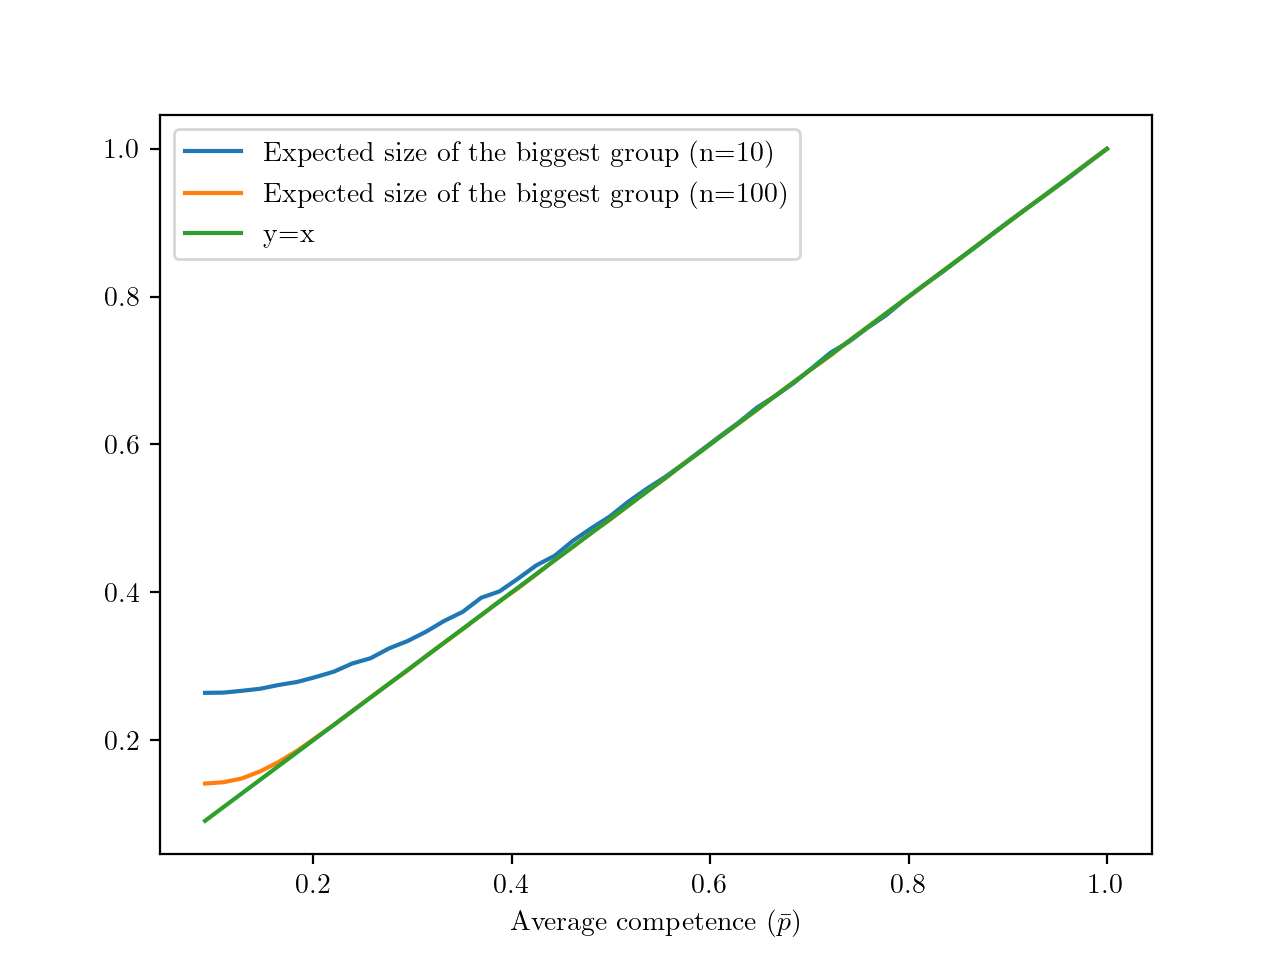
\includegraphics[width=0.75\linewidth]{figures/Benoit_biggest_group} \hfill{}

\caption{Expected size of the majority depending on average competence, with \(n=10\) (blue) and \(n=100\) (orange).}\label{fig:biggestgroup}
\end{figure}

\subsubsection{Inferring within population competence}\label{inferring-within-population-competence}

Here, we focus on one individual and we aim to infer his personal level of competence \(p\). We observe the number \(K\) of individuals who agree with him. Either the focus individual is right (which happens with probability \(p\)) and \(K\) follows a binomial distribution of parameters \(n\) and \(\bar p\); or the individual is wrong (which happens with probability \(1-p\)) and then \(K\) follows a binomial distribution of parameters \(n\) and \(\bar q\). Thus, \(K\) follows a mixture distribution of different parameters, with weights \(p\) and \(1-p\).

Using the mixture distributions property, we can compute the mean of \(K\):
\[
E(K) = n(p \bar p + (1-p)\bar q) = n(p (\bar p - \bar q) + \bar q)
\]

Clearly, \(E(K)\) increases with \(p\) if and only if \(\bar p - \bar q > 0\). In other words, if the population is better than chance, then we expect that the more competent an individual is, the more people agree with him.

But now, what exactly can we infer from \(p\) by observing \(K\)? To answer that, we need to assume a distribution of competence levels in the population, that we will also use as a prior. We assume that in the competence levels are distributed as a beta distribution, of parameters \(\alpha\) and \(\beta\). Their density is \(f(x) = x^\alpha(1-x)^\beta\). Then, \(\bar p = \frac{\alpha}{\alpha+\beta}\), the mean of our beta distribution.

Using Bayes formula, we can write the posterior distribution of \(p\):
\[
\Pi(x|K=k) \propto f(x)P(K=k|p=x) = f(x)(x\bar p^k(1-\bar p)^{n-k} + (1-x)\bar q^k (1-\bar q)^{n-k})
\]

\[
= x^{\alpha+1}(1-x)^\beta[\bar p^k(1-\bar p)^{n-k}] + x^{\alpha}(1-x)^{\beta+1} [\bar q^k (1-\bar q)^{n-k}]
\]
We recognise a mixture distribution between two beta distributions, with parameters \(\alpha+1\) and \(\beta\) for the first one, \(\alpha\) and \(\beta + 1\) for the second. The first one has a bigger mean than our original Beta(\(\alpha\),\(\beta\)) distribution, the second a lower one (see Fig. \ref{fig:posterior}). In a way, the bayesian updating shifts the distribution to the right or to the left, depending on \(K\).



\begin{figure}

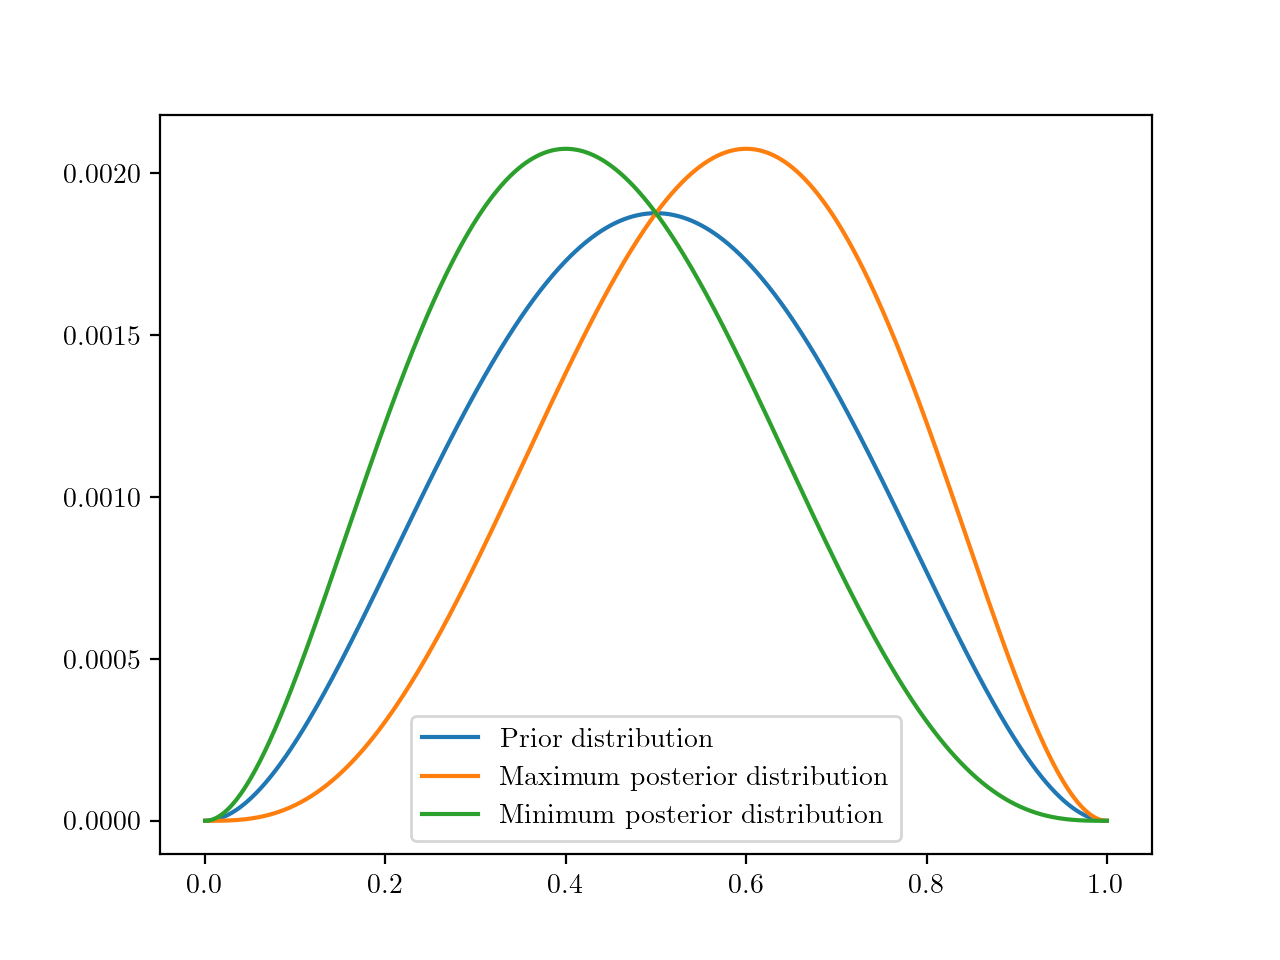
\includegraphics[width=0.75\linewidth]{figures/Benoit_posterior} \hfill{}

\caption{Prior and boundary posterior distributions. These distributions are the limit distributions when the individual is either part of a consensus or a dissensus, and when \(\bar p \gg \bar q\) or \(n\) is large. Here, \(\alpha=\beta=2\) and we do not need to define the other parameters. As we explain below, the prior distribution determines the range between the possible posterior distributions.}\label{fig:posterior}
\end{figure}

The weightings (\(\bar p^k(1-\bar p)^{n-k}\) and \(\bar q^k (1-\bar q)^{n-k}\) correspond to the probability that \(k\) individuals choose the right answer, and a particular wrong answer, respectively (we took out the binomial coefficients, who are equal for both answer types). Since \(\bar p > \bar q\), the former is much stronger for large \(k\), and the latter much stronger for low \(k\). For \(k=n\) (i.e.~when the focus individual is part of a consensus), the ratio of weighting if \((p/q)^n\), which is very large when \(n\) is large or when \(\bar p \gg \bar q\). In this case, for high \(k\), the posterior distribution is well approximated by a Beta(\(\alpha+1\),\(\beta\)). Conversely, when \(k\) is close to zero (and when the other conditions are present), the posterior distribution is well approximated by a Beta(\(\alpha\),\(\beta+1\)).

We can plot the mean of the posterior distribution, which can be interpreted as the average estimation we can make of the individual competence, depending on \(K\) (Fig. \ref{fig:competence-k}). For low \(n\) and \(m\) (the main experiment used \(n=m=2\), the function is not too steep. For higher values, it gets sigmoidal, or even a jump function.



\begin{figure}

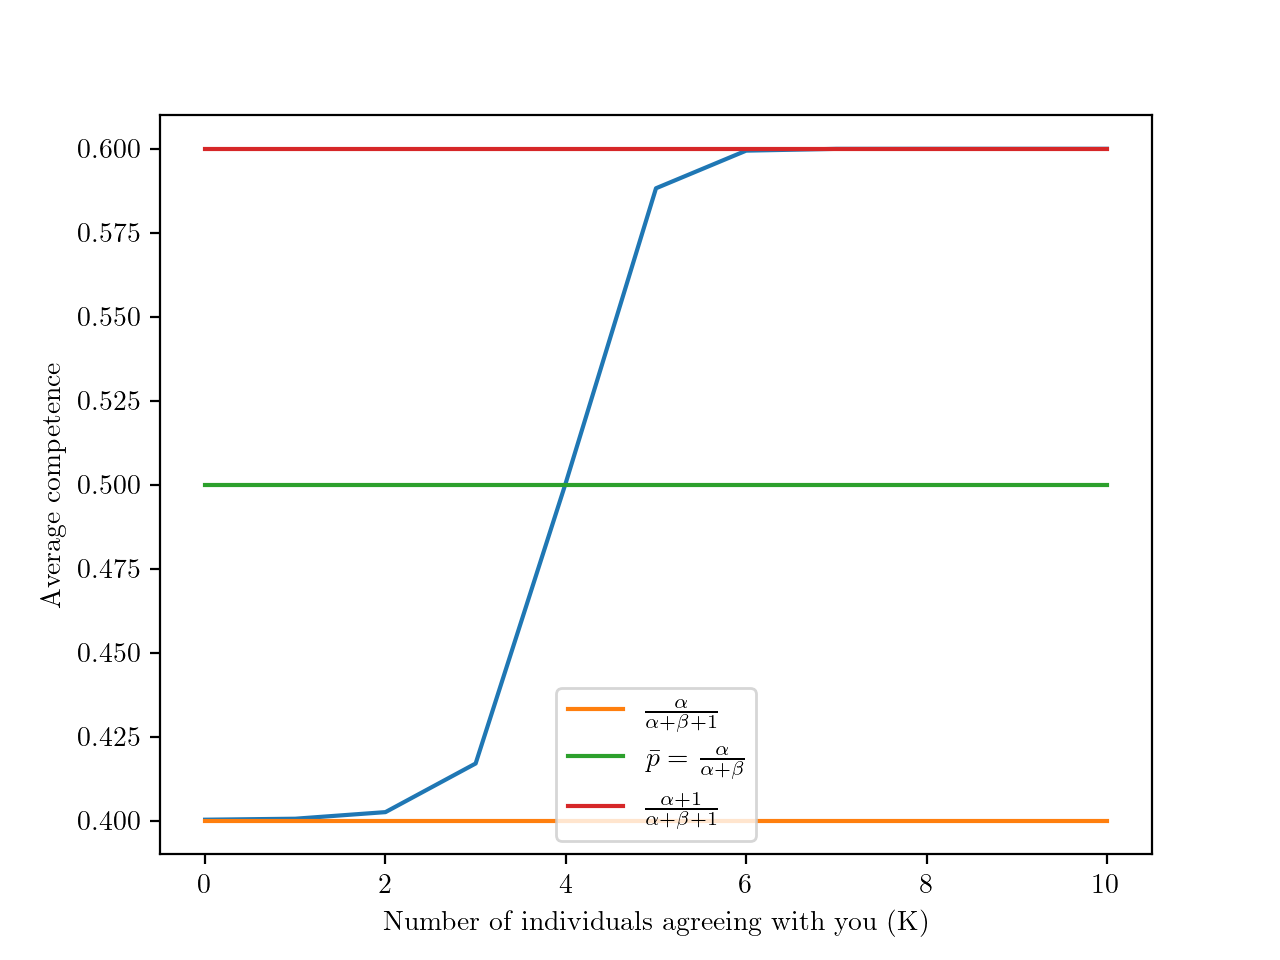
\includegraphics[width=0.75\linewidth]{figures/Benoit_competence_k} \hfill{}

\caption{Mean of the posterior competence distribution, depending on the number of individuals agreeing with the focus individual. Here, \(n=m=10\).}\label{fig:competence-k}
\end{figure}

How much we learn from the observation depends crucially on \(\alpha\) and \(\beta\), that is, on the prior distribution of competence in the population. The range of possible mean estimates is \(\frac{1}{\alpha+\beta + 1}\), it is larger when \(\alpha\) and \(\beta\) are low.

For instance, let us set \(\alpha=\beta\) (which implies \(\bar p = \frac 12\)). Now, we vary the two shape parameters from close to 0 (beta distributions need positive shape parameters) to a large number. This shifts the distribution from a bimodal one (with \(\alpha=\beta \approx 0\), the distribution is perfectly bimodal, with half of the population always right and the other half always right) to a sharp unimodal distribution (when \(\alpha\) and \(\beta\) are large, the whole population has basically a competence of .5). The more bimodal the distribution, the larger the range of possible estimates (Fig. \ref{fig:update}). In the limit, when \(\alpha\) and \(\beta\) are close to 0, we can infer that an individual is either perfectly competent or perfectly incompetent, depending on whether they are part of a consensus or alone in their opinion. On the contrary, when \(\alpha\) and \(\beta\) are large, we do not change our estimate at all as the distribution is concentrated around .5. Intuitively, this makes sense: If we assume everyone is equally (in)competent, with no exception, we wouldn't infer anything from observing a convergence.



\begin{figure}

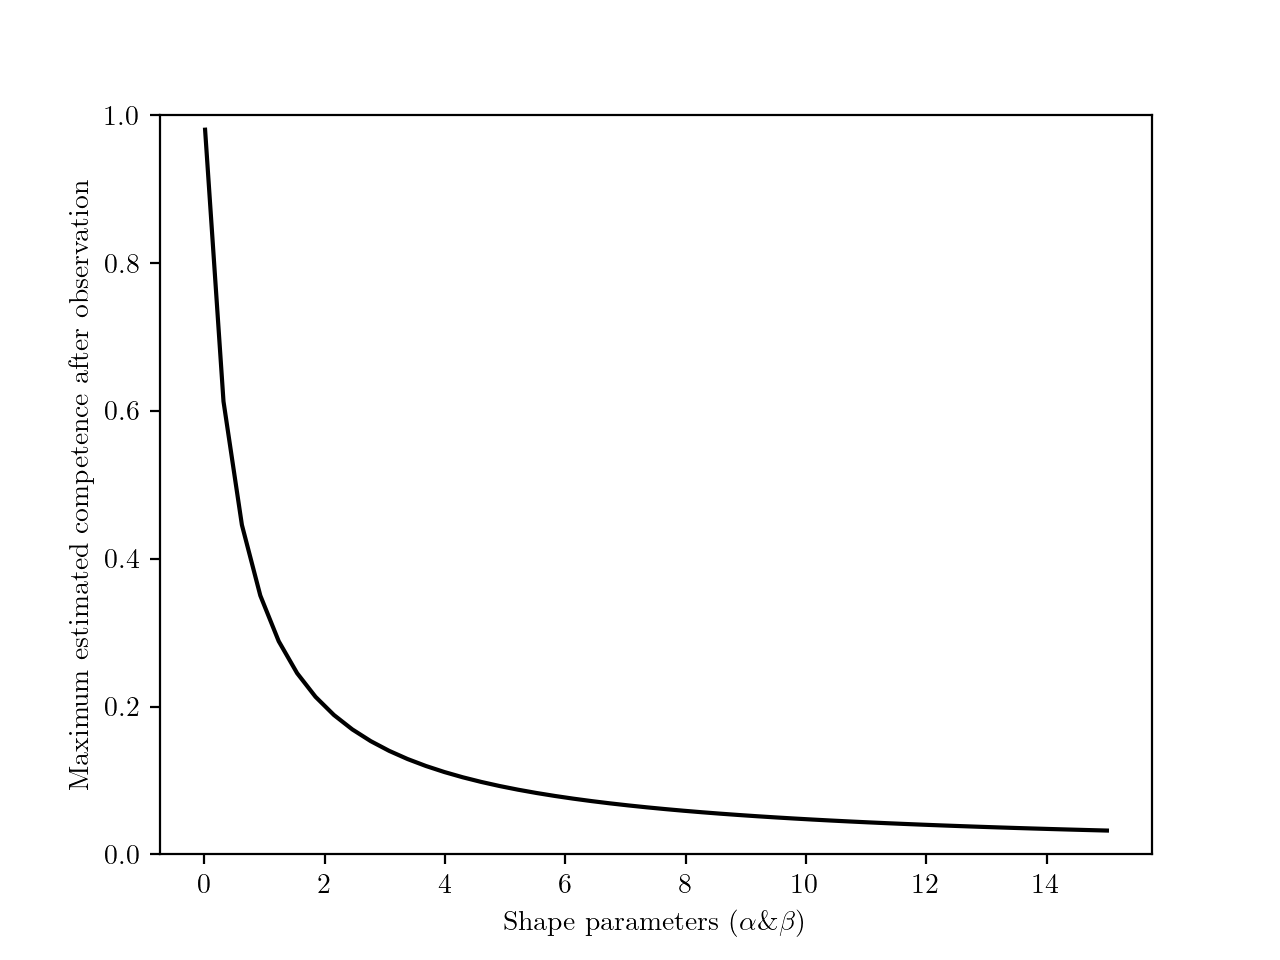
\includegraphics[width=0.75\linewidth]{figures/Benoit_update} \hfill{}

\caption{Range of possible estimates (difference between the minimum and the maximum estimate), depending on the shape of the distribution (here, we assume that \(\alpha=\beta\)).}\label{fig:update}
\end{figure}

\subsubsection{Inferring accuracy}\label{inferring-accuracy}

Now, instead of inferring competence, we want to infer accuracy, i.e.~the probability that an individual answer is correct.

Again, using Bayes formula, we have:

\[
p(right|K=k) = \frac{p(K=k|right)p(right)}{p(K=k)} = \frac{\bar p (\bar p^{k-1} (1-\bar p)^{n-k})}{((\bar p^k (1-\bar p)^{n-k}) + (\bar q^k (1-\bar q)^{n-k}))} 
\]

\[
= \frac{1}{1 +  (\bar p/\bar q)^k \left( \frac{1-\bar q}{1-\bar p}\right)^{n-k} }
\]

Compared to competence, it is clear (Figure \ref{fig:accuracy}) that accuracy can be inferred much more strongly.



\begin{figure}

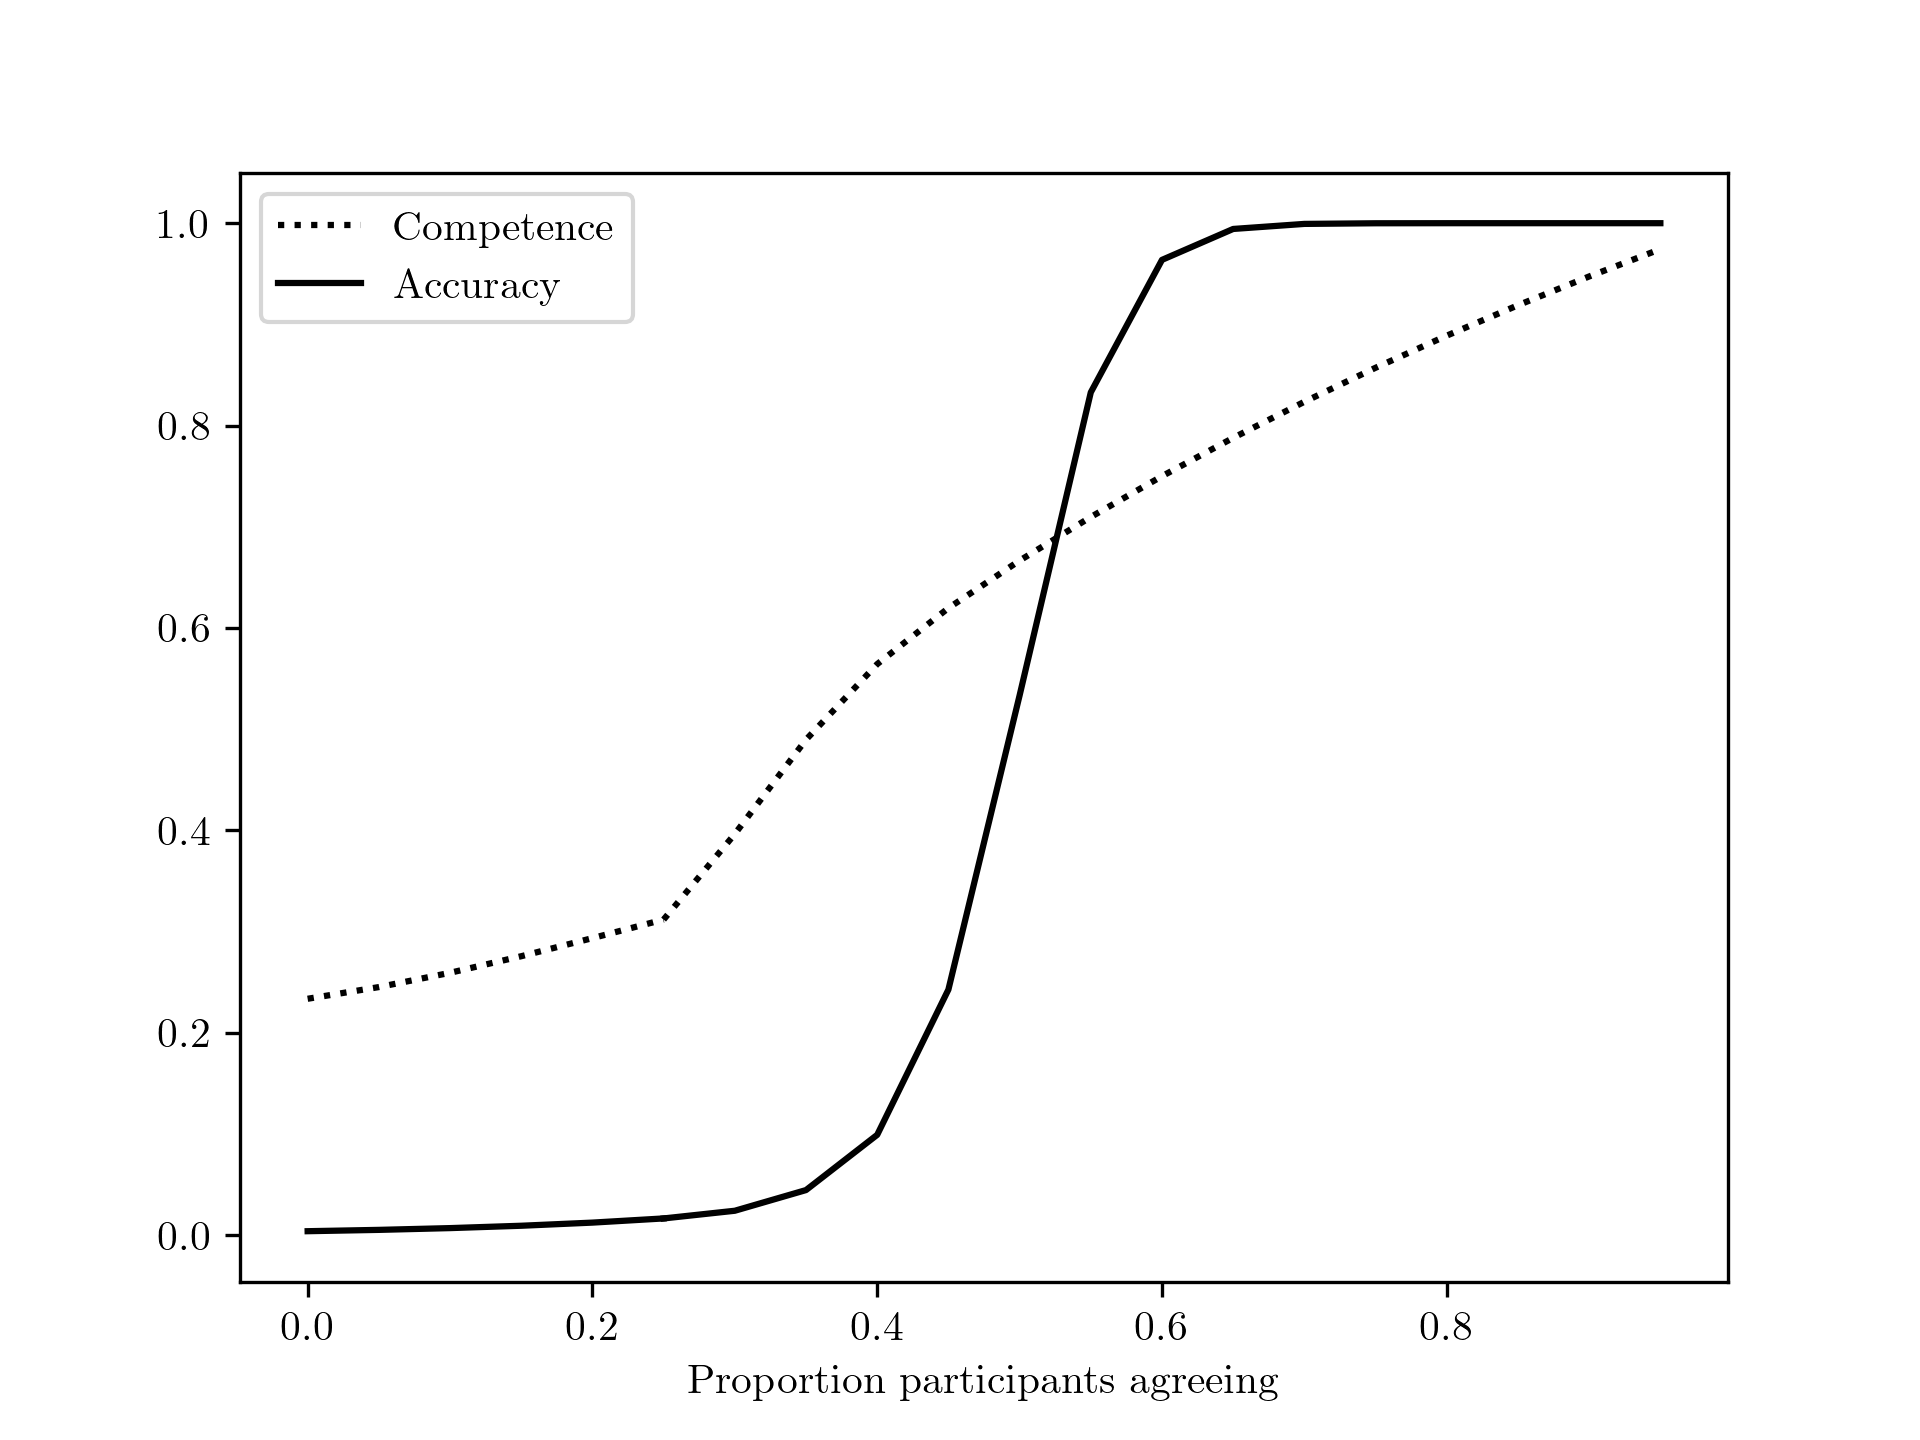
\includegraphics[width=0.75\linewidth]{figures/Benoit_accuracy} \hfill{}

\caption{Estimated competence and accuracy depending on the degree of consensus. Here, we assume that \(\alpha=1\), \(n=20\) and \(m=4\). \(\beta\) is inferred from \(\alpha\) and the majority size.}\label{fig:accuracy}
\end{figure}

\subsection{Continuous choices}\label{continuous-choices}

A group of \(N\) individuals makes a prediction. The right answer is \(\theta\), we assume their answers \(x_i, i \in 1,…,N\) are normally distributed around \(\theta\), with a variance \(\sigma^2\) reflecting the group incompetence (so the lower \(\sigma^2\), the more the group can be said to be competent).

We estimate the degree of divergence through the unbiased sample variance \(\hat \sigma^2\), defined as the average squared distance to the sample mean \(\bar x =\frac 1 n \sum_{i=1}^n x_i\):

\[\hat \sigma^2 = \frac 1 {n-1} \sum_{i=1}^n (x_i - \bar x)^2\]

It is well known that \(\hat \sigma^2\) (when coupled with the sample mean) is a ``sufficient'' estimator of \(\sigma^2\), that is, it contains all the available information about \(\sigma^2\). It follows, from the Lehmann-Scheffé theorem, that it is also the minimum-variance unbiased estimator, that is, the most precise way to estimate \(\sigma^2\) while staying unbiased.

\clearpage
\newpage

\section{Simulations}\label{simulations}

Are we justified in inferring competence and accuracy from convergence? To complement our analytical argument, we ran simulations, intended to mirror our experimental setup. We find that--under certain conditions--more convergent groups indeed tend to be more competent and accurate. In this appendix, we describe these simulations in detail.

\subsection{Numerical choice context}\label{numerical-choice-context}

When several people estimate a quantity (numeric scenario), their convergence can be measured for example by the empirical variance. The closer the estimates, i.e.~the smaller the empirical variance, the greater convergence. This measure is at the group level.

To provide a normative answer, we ran simulations for a scenario in which individuals provide an estimate on a scale from 1000 to 2000. In our simulations, we suppose that an individual's answer is drawn from a normal distribution. Each individual has their own normal distribution. All normal distributions are centered around the true answer - but they differ in their standard deviations. The value of that standard deviation is what we define as an individual's competence. The lower the standard deviation, the higher the competence, i.e.~the more likely a guess drawn from the normal distribution will be close to the true answer. We (arbitrarily) define a range of competence: we set the lowest competence equal to the range of possible values, i.e.the largest standard deviation (2000 - 1000) = 1000. We set the highest competence to 0.1\% of the range of possible values, i.e.the smallest standard deviation (0.001 x 1000) = 1 (see Fig. \ref{fig:example-competence-numeric}).



\begin{figure}
\includegraphics[width=0.75\linewidth]{output/figures/example-competence-numeric} \caption{Range of possible data generating functions for individuals.}\label{fig:example-competence-numeric}
\end{figure}

We suppose that individual competence levels are drawn from a competence distribution, which can be expressed by a beta distribution. This competence distribution can take vary different shapes, depending on the alpha and beta parameters that describe the distribution (see Fig. \ref{fig:simulations}).

We draw an estimate for each individual based on their respective competence distribution. For each individual, we then measure accuracy as the (squared) distance between their estimate and the true answer. Having a competence and an accuracy value for each individual, we randomly assign individuals to groups of three. For each group, we calculate the average of the three individuals' competence and accuracy. We measure the convergence of a group by calculating the standard deviation of the estimates. We run this simulation on a sample size of roughly 99900 (varying slightly as a function of sample size). We repeat this simulation process for various sample sizes and competence distributions. The results are displayed in Fig. \ref{fig:simulation-accuracy-numeric} for accuracy, and Fig. \ref{fig:simulation-competence-numeric} for competence. Across all underlying competence distributions, we find a positive correlation between convergence and accuracy, which tends towards 1 as sample size increases (see Fig. \ref{fig:simulation-numeric-correlations}). As for competence, we find a positive correlation between convergence and competence across all underlying competence distributions. However, these correlations are weaker than for accuracy, and do not increase with sample size (see Fig. \ref{fig:simulation-numeric-correlations}).



\begin{figure}
\includegraphics[width=0.75\linewidth]{output/figures/simulation-numeric-correlations} \caption{Correlation between the convergence of the answers of a group of agents and (left) the average accuracy of their answers; (right) the average competence of the agents, as a function of how many agents are in the group, and of the competence distribution of the agents (see Fig. \ref{fig:simulations}).}\label{fig:simulation-numeric-correlations}
\end{figure}

\subsection{Categorical choice context}\label{categorical-choice-context}



\begin{figure}
\includegraphics[width=1\linewidth]{output/figures/simulation-accuracy-sample-categorical} \caption{Accuracy as a function of convergence, for different population competence distributions and sample sizes. The number of choice options is three.}\label{fig:simulation-accuracy-sample-categorical}
\end{figure}



\begin{figure}
\includegraphics[width=1\linewidth]{output/figures/simulation-competence-sample-categorical} \caption{Competence as a function of convergence (i.e.~vote share for an option), for different population competence distributions and sample sizes. The number of choice options is three.}\label{fig:simulation-competence-sample-categorical}
\end{figure}

When people make a choice based on several categories, their answers cannot be ranked by their nature (i.e.~they are nominal, not ordinal), and that there are fewer of them (e.g.~one of three possible products to choose, instead of an estimate between one and two thousand). In this case, convergence can be measured by the share of people agreeing on an answer. The larger the share of informants agreeing on an answer, the greater convergence. This measure is at the response level, nested within the group level.

As for the numeric scenario, we ran simulations to provide a normative answer as to whether it is justified to infer accuracy and competence from greater convergence. We, again, suppose that an individual's answer is drawn from an internal distribution - in this case, a multinomial distribution, that describes how likely the individual is to choose each available option. If there are m choice options, an individual has the probability p of picking the right one, and the probability of (1-p)/(m-1) to pick any other option. Each individual has their own multinomial distribution. We define competence as the probability of making the correct choice. The higher the competence, the greater the probability that an individual will choose the correct option. Competence values range from being at chance for selecting the correct option (p = 1/m) to certainly selecting the correct option (p = 1). As before in the numeric case, suppose that individual competence levels are drawn from a competence distribution, which can be expressed by a beta distribution (see Fig. \ref{fig:simulations}). Based on their competence level, we draw an estimate for each individual. We measure an individual's accuracy as a binary outcome, namely whether they picked the correct option, or not. We then randomly assign individuals to groups of informants (we vary the sample size from one simulation to another). Within these groups, we calculate the share of individuals voting for an answer option. For example, in a scenario in which three individuals pick among three options (A, B and C), two individuals might vote C and one B. In this case we obtain an average accuracy and an average competence value for a share of 2/3 (option C) and for a share of 1/3 (option B). We simulate this on a population of 99900 individuals. We repeat this procedure varying the underlying population competence distributions, and additionally varying either (a) the sample size of informants, or (b) the number of choice options. If we vary the sample size, we hold the number of choice options constant at n = 3, and vice versa when varying the number of choice options. Fig. \ref{fig:simulation-accuracy-sample-categorical} shows the average accuracy, and Fig. \ref{fig:simulation-competence-sample-categorical} the average competence value for each share of votes, for different competence levels and varying the sample size. Fig. \ref{fig:simulation-accuracy-options-categorical} and Fig. \ref{fig:simulation-competence-options-categorical} display the same relationship, but varying the number of choice options instead. The figures display that, across all sample sizes and competence levels, the larger the share of votes for an option, the more accurate the option is on average. That relationship appears to follow some sigmoid curve which switches from an average accuracy of 0 to an average accuracy of 1 before a share of 0.5 is attained, and which is steeper for larger sample sizes. For competence, we observe a similar sigmoid-like relationship, but of lesser amplitude and varying considerably as a function of the underlying population competence distributions.



\begin{figure}
\includegraphics[width=0.75\linewidth]{output/figures/simulation-accuracy-options-categorical} \caption{Accuracy as a function of vote share for an option, for different population competence distributions and number of choice options. Points represent averages across all simulations within the respective segment. The sample size is three.}\label{fig:simulation-accuracy-options-categorical}
\end{figure}



\begin{figure}
\includegraphics[width=0.75\linewidth]{output/figures/simulation-competence-options-categorical} \caption{Competence as a function of vote share for an option, for different population competence distributions and number of choice options. Points represent averages across all simulations within the respective segment. The sample size is three.}\label{fig:simulation-competence-options-categorical}
\end{figure}

In sum, given the set of specific assumptions we made, our simulations suggest that people are indeed justified in inferring accuracy and competence from convergence in both numeric and categorical choice settings.



\begin{figure}
\centering
\includegraphics{output/figures/simulation-accuracy-numeric.pdf}
\caption{\label{fig:simulation-accuracy-numeric}Simulation results showing the relationship between convergence and accuracy for different population competence distributions.}
\end{figure}



\begin{figure}
\centering
\includegraphics{output/figures/simulation-competence-numeric.pdf}
\caption{\label{fig:simulation-competence-numeric}Simulation results showing the relationship between convergence and competence for different population competence distributions.}
\end{figure}

\clearpage

\section{Experiment 1}\label{exp1}

\subsection{Stimuli}\label{stimuli}

\FloatBarrier

The means of the normal distributions that we draw our estimates from were distinct between sets of estimates. Considering our within-participant design, we wanted to ensure that participants understood each set of estimates as being the result of a different, unrelated game. In order to assure that random draws from the distributions will (most likely) appear on the response scale (1000 to 2000), we constrained the means of all normal distributions to lie between the first and third quartile of the response scale (i.e.~smallest possible mean was 1225 and largest 1775). We define a set of eight means--one for each set of estimates--that cover the range from first to third quartile of the predefined scale with an equal interval (1250, 1325, 1400, 1475, 1550, 1625, 1700, 1775). We randomly paired means with conditions when generating the stimuli. We then drew the set of estimates from the respective normal distributions given the assigned means and the condition constraints. We repeated this three times, resulting in three different series of eight sets of estimates. We randomly assign participants to one of these series. Additionally, for each participant, we randomize the order of appearance of the sets of estimates within the respective series. Images of all sets of estimates can be found on the OSF.

\subsection{Attention check}\label{attention-check}

Imagine you are playing video games with a friend and at some point your friend says: ``I don't want to play this game anymore! To make sure that you read the instructions, please write the three following words''I pay attention'' in the box below. I really dislike this game, it's the most overrated game ever.''

Do you agree with your friend? (Yes/No)

\subsection{Results}\label{results}

Figure \ref{fig:exp1-plot} visualizes the results and table \ref{tab:exp1-table} contains descriptive results. Figure \ref{fig:exp1-outcomes} visualizes score differences between the two outcomes, accuracy and competence.

\begin{table}[tbp]

\begin{center}
\begin{threeparttable}

\caption{\label{tab:exp1-table}}

\begin{tabular}{llll}
\toprule
Convergence & \multicolumn{1}{c}{Number} & \multicolumn{1}{c}{Accuracy} & \multicolumn{1}{c}{Competence}\\
\midrule
divergent & small & 3.152 (sd = 1.495) & 3.57 (sd = 1.341)\\
divergent & large & 3.232 (sd = 1.282) & 3.465 (sd = 1.184)\\
convergent & small & 4.425 (sd = 1.461) & 4.695 (sd = 1.221)\\
convergent & large & 4.695 (sd = 1.424) & 4.805 (sd = 1.251)\\
\bottomrule
\end{tabular}

\end{threeparttable}
\end{center}

\end{table}



\begin{figure}
\centering
\includegraphics{output/figures/exp1-plot.pdf}
\caption{\label{fig:exp1-plot}Distributions of accuracy and competence by level of convergence.}
\end{figure}

\subsection{Research questions}\label{research-questions}

We had three additional research questions regarding the number of informants:

\textbf{\emph{RQ1: Do H1 and H2 hold for both a small {[}3{]} and a large {[}10{]} number of estimates?}}

\textbf{\emph{RQ2: When making a guess based on the opinions of (independent) informants, will participants be more confident about their guess when there is a larger number of estimates compared to when this number is smaller?}}

\textbf{\emph{RQ3: Is there an interaction effect between the number of estimates and convergence on perceived competence of informants?}}

Regarding RQ1, we ran the same mixed models as for the two hypotheses, but without number as a covariate. Instead, we ran separate models for the three and the ten informants conditions. We find that for both sub-samples, there is a positive effect of convergence on both accuracy (\(\hat{b}_{\text{three informants}}\) = 1.27 {[}1.112, 1.433{]}, p = \textless{} .001; \(\hat{b}_{\text{ten informants}}\) = 1.46 {[}1.285, 1.64{]}, p = \textless{} .001) and competence (\(\hat{b}_{\text{three informants}}\) = 1.12 {[}0.955, 1.295{]}, p = \textless{} .001; \(\hat{b}_{\text{ten informants}}\) = 1.34 {[}1.142, 1.538{]}, p = \textless{} .001).

To test the other two research questions, we ran the same mixed-models as for the hypotheses, but this time including an interaction between number of informants and convergence. We use deviation-coded versions of our convergent variable (divergent = -0.5, convergent = 0.5), allowing us to have a coefficient measuring the main effect of the number of informants in our model. Regarding RQ2, pooling across convergent and divergent conditions, we find a main effect of number, such that participants had more confidence in their estimate when they relied on ten informants compared to three informants (\(\hat{b}_{\text{Accuracy}}\) = 0.18 {[}0.076, 0.274{]}, p = \textless{} .001). Regarding RQ3, we find an interaction between number of informants and convergence on competence: the positive effect of convergence was stronger in scenarios involving ten informants compared to three informants (\(\hat{b}_{\text{Competence}}\) = 0.22 {[}0.028, 0.402{]}, p = 0.024). We do not find a statistically significant interaction on accuracy (\(\hat{b}_{\text{Accuracy}}\) = 0.19 {[}-0.007, 0.387{]}, p = 0.059).



\begin{figure}
\centering
\includegraphics{output/figures/exp1-outcomes.pdf}
\caption{\label{fig:exp1-outcomes}Differences between accuracy and competence ratings, by level of convergence.}
\end{figure}

\subsection{Minor deviation from preregistration}\label{minor-deviation-from-preregistration}

In our preregistration, we stated we would run paired t-tests and only conduct mixed models as a robustness check. However, it became clear to us later that mixed models are more appropriate in light of our data structure. In the main article, we therefore only report the results of the mixed models. Note, however, that using paired t-tests, we confirm our results (Accuracy: 1.37, t-statistic = 26.14, p \textless{} .001; Competence: 1.23, t-statistic = 21.82, p \textless{} .001)

\subsection{Sensitivity simulation}\label{sensitivity-simulation}

We had based our power calculations on a paired t-test (using the widely used tool G*Power), which does not correspond to the mixed-models we eventually ran. To address this point, here, we seek to identify the minimum effect size that our analysis with mixed models could have detected, given a 90\% power, an N of 200 participants, and other parameters derived from the estimates observed in the sample of Experiment 1 (see \ref{tab:exp1-regression-table}). By contrast to a standard power simulation (which varies sample size), a sensitivity simulation varies the effect size, while holding the sample size and desired power constant.

\begin{table}
\centering
\caption{\label{tab:exp1-regression-table}Model Results Experiment 1}
\centering
\begin{tabular}[t]{lcc}
\toprule
  & Accuracy & Competence\\
\midrule
(Intercept) & 3.105 & 3.516\\
 & (0.077) & (0.068)\\
convergenceconvergent & 1.368 & 1.232\\
 & (0.072) & (0.085)\\
numberlarge & 0.175 & 0.002\\
 & (0.050) & (0.048)\\
SD (Intercept ID) & 0.905 & 0.764\\
SD (convergenceconvergent ID) & 0.732 & 0.993\\
Cor (Intercept\textasciitilde{}convergenceconvergent ID) & -0.128 & -0.554\\
SD (Observations) & 1.006 & 0.955\\
\midrule
Num.Obs. & 1600 & 1600\\
R2 Marg. & 0.191 & 0.195\\
R2 Cond. & 0.594 & 0.532\\
AIC & 5131.0 & 4950.5\\
BIC & 5168.7 & 4988.1\\
ICC & 0.5 & 0.4\\
RMSE & 0.91 & 0.86\\
\bottomrule
\end{tabular}
\end{table}



\begin{figure}
\centering
\includegraphics{output/figures/sensitivity.pdf}
\caption{\label{fig:sensitivity}Results of the sensitivity analysis.}
\end{figure}

The results of this can be seen in Fig. \ref{fig:sensitivity}. In our sample, we found a statistically significant effect size of 1.37 for accuracy and an effect size of 1.23 for competence (both on their original scales from 1 to 7). The simulations show that, given our parameter assumptions (based on the observations in our sample) and a sample size of N = 200, we would have detected an effect as small as 0.4 with a power of at least 90\% (in fact nearly 100\%) for both accuracy and competence.

\clearpage

\section{Experiment 2}\label{exp2}

\FloatBarrier

\subsection{Attention check}\label{attention-check-1}

Imagine you are playing video games with a friend and at some point your friend says: ``I don't want to play this game anymore! To make sure that you read the instructions, please write the three following words''I pay attention'' in the box below. I really dislike this game, it's the most overrated game ever.''

Do you agree with your friend? (Yes/No)

\subsection{Results}\label{results-1}

Figure \ref{fig:exp2-plot} visualizes the results and table \ref{tab:exp2-table} contains descriptive results.

\begin{table}[tbp]

\begin{center}
\begin{threeparttable}

\caption{\label{tab:exp2-table}}

\begin{tabular}{lll}
\toprule
Independence & \multicolumn{1}{c}{Accuracy} & \multicolumn{1}{c}{Competence}\\
\midrule
dependent & 4.03 (sd = 1.389) & 4.48 (sd = 1.022)\\
independent & 3.775 (sd = 1.502) & 4.36 (sd = 0.967)\\
\bottomrule
\end{tabular}

\end{threeparttable}
\end{center}

\end{table}



\begin{figure}
\centering
\includegraphics{output/figures/exp2-plot.pdf}
\caption{\label{fig:exp2-plot}Distributions of accuracy and competence by level of informational dependency.}
\end{figure}

\clearpage

\section{Experiment 3}\label{exp3}

\FloatBarrier

\subsection{Attention check}\label{attention-check-2}

Imagine you are playing video games with a friend and at some point your friend says: ``I don't want to play this game anymore! To make sure that you read the instructions, please write the three following words''I pay attention'' in the box below. I really dislike this game, it's the most overrated game ever.''

Do you agree with your friend? (Yes/No)

\subsection{Stimuli}\label{stimuli-1}

Our design required that each participant sees four different sets of predictions--two convergent and two divergent ones. We generated new stimuli: As in experiment 1, estimates would appear on a scale from 1000 to 2000. By contrast with experiment 1, we generated the sets of estimates with random draws from uniform distributions (instead of normal distributions). We varied the range of these distributions according to convergence (60 for convergence, 600 for divergence). Switching from normal distributions to uniform distributions made `unlucky' draws in which conditions are visually not distinguishable less likely. And additional difference to experiment one was that all scenarios only involved groups of three informants (never ten).

Similar to the previous experiments, we also vary the value on the prediction scale (from 1000 to 2000) across which the range is centered. Considering our within-participant design, this, again, made it seem more likely that participants understand each set of predictions as being the result of a different stock, with a different true value. In order to assure all random draws from the distributions would appear on the response scale, we constrained the center of the uniform distributions to lie between 1300 and 1700. We define four center values -- one per set of predictions -- that divide this interval in (rounded) quartiles (1300, 1430, 1570, 1700). Given a center and a range, we then draw the predictions from uniform distributions. For example, in a draw for a divergent set of estimates with a center of 1700, each value within a range of 1400 and 2000 is equally likely to get selected. To avoid that single draws overlap too much within the same set, we defined a minimum space of 5 between the three predictions of a set.

To minimize confounding of convergence with a certain placement of the center value, we paired center values with conditions such that each condition appears once in each half of the scale and each condition gets one of the extreme values. For example, in one set the convergence condition would get assigned center values of 1300 and 1570, the divergent condition center values of 1430 and 1700). We generated four such series (all possible combinations) and randomly assigned participants to one of them. Additionally, for each participant, we randomized the order of appearance of the sets of predictions within the respective series.

For each set of predictions, we calculated the empirical mean based on the randomly drawn estimates. In the conflict of interest condition, this mean was inserted as the value that participants were be told experts would gain from. Consequently, the convergent predictions converge around what is said to be the incentivized value for the experts to choose.

\subsection{Results}\label{results-2}

Table \ref{tab:exp3-table} contains descriptive results.

\begin{table}
\centering
\caption{\label{tab:exp3-table}}
\centering
\begin{tabular}[t]{lllll}
\toprule
\multicolumn{1}{c}{} & \multicolumn{2}{c}{Accuracy} & \multicolumn{2}{c}{Competence} \\
\cmidrule(l{3pt}r{3pt}){2-3} \cmidrule(l{3pt}r{3pt}){4-5}
  & Divergent & Convergent & Divergent & Convergent\\
\midrule
Conflict of interest & 3.566 (sd = 1.215) & 4.455 (sd = 1.409) & 3.732 (sd = 1.101) & 4.556 (sd = 1.19)\\
Independent & 3.4 (sd = 1.08) & 5.28 (sd = 1.052) & 3.61 (sd = 1.111) & 5.235 (sd = 0.992)\\
\bottomrule
\end{tabular}
\end{table}

\clearpage

\section{Experiment 4}\label{exp4}

\FloatBarrier

\subsection{Attention check}\label{attention-check-3}

Imagine you are playing video games with a friend and at some point your friend says: ``I don't want to play this game anymore! To make sure that you read the instructions, please write the three following words''I pay attention'' in the box below. I really dislike this game, it's the most overrated game ever.''

Do you agree with your friend? (Yes/No)

\subsection{Stimuli}\label{stimuli-2}

We manipulate convergence within participants. All participants see all four conditions, with two stimuli (i.e.~game results) per condition (see Table \ref{tab:exp4-stimuli}). Each participant therefore sees eight stimuli in total (4 convergence levels x 2 stimuli)

\begin{longtable}[]{@{}
  >{\centering\arraybackslash}p{(\columnwidth - 4\tabcolsep) * \real{0.1007}}
  >{\centering\arraybackslash}p{(\columnwidth - 4\tabcolsep) * \real{0.4497}}
  >{\centering\arraybackslash}p{(\columnwidth - 4\tabcolsep) * \real{0.4497}}@{}}
\caption{\label{tab:exp4-stimuli}All stimuli by levels of convergence}\tabularnewline
\toprule\noalign{}
\begin{minipage}[b]{\linewidth}\centering
Level
\end{minipage} & \begin{minipage}[b]{\linewidth}\centering
Version a)
\end{minipage} & \begin{minipage}[b]{\linewidth}\centering
Version b)
\end{minipage} \\
\midrule\noalign{}
\endfirsthead
\toprule\noalign{}
\begin{minipage}[b]{\linewidth}\centering
Level
\end{minipage} & \begin{minipage}[b]{\linewidth}\centering
Version a)
\end{minipage} & \begin{minipage}[b]{\linewidth}\centering
Version b)
\end{minipage} \\
\midrule\noalign{}
\endhead
\bottomrule\noalign{}
\endlastfoot
minority (0) & 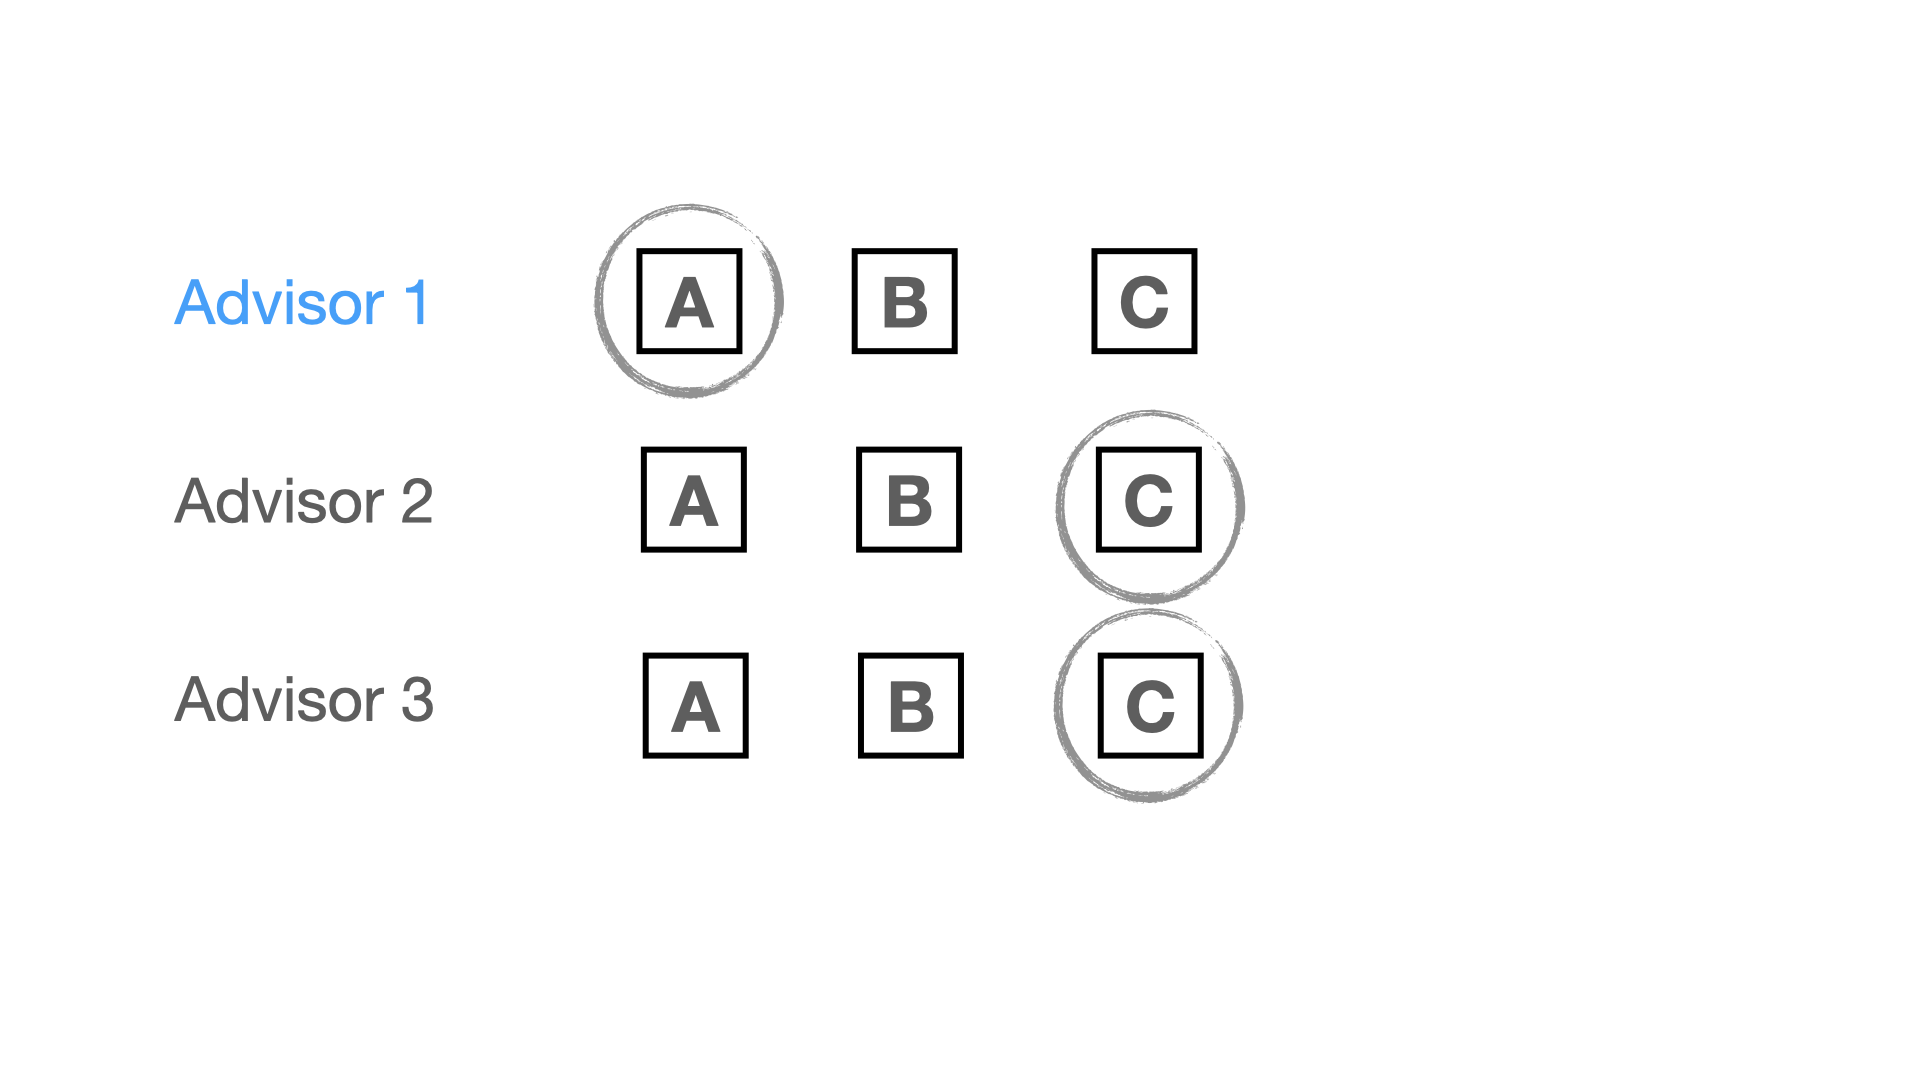
\includegraphics[width=0.6\textwidth,height=\textheight]{Experiment_4/figures/stimuli/opp_majority_a.png} & 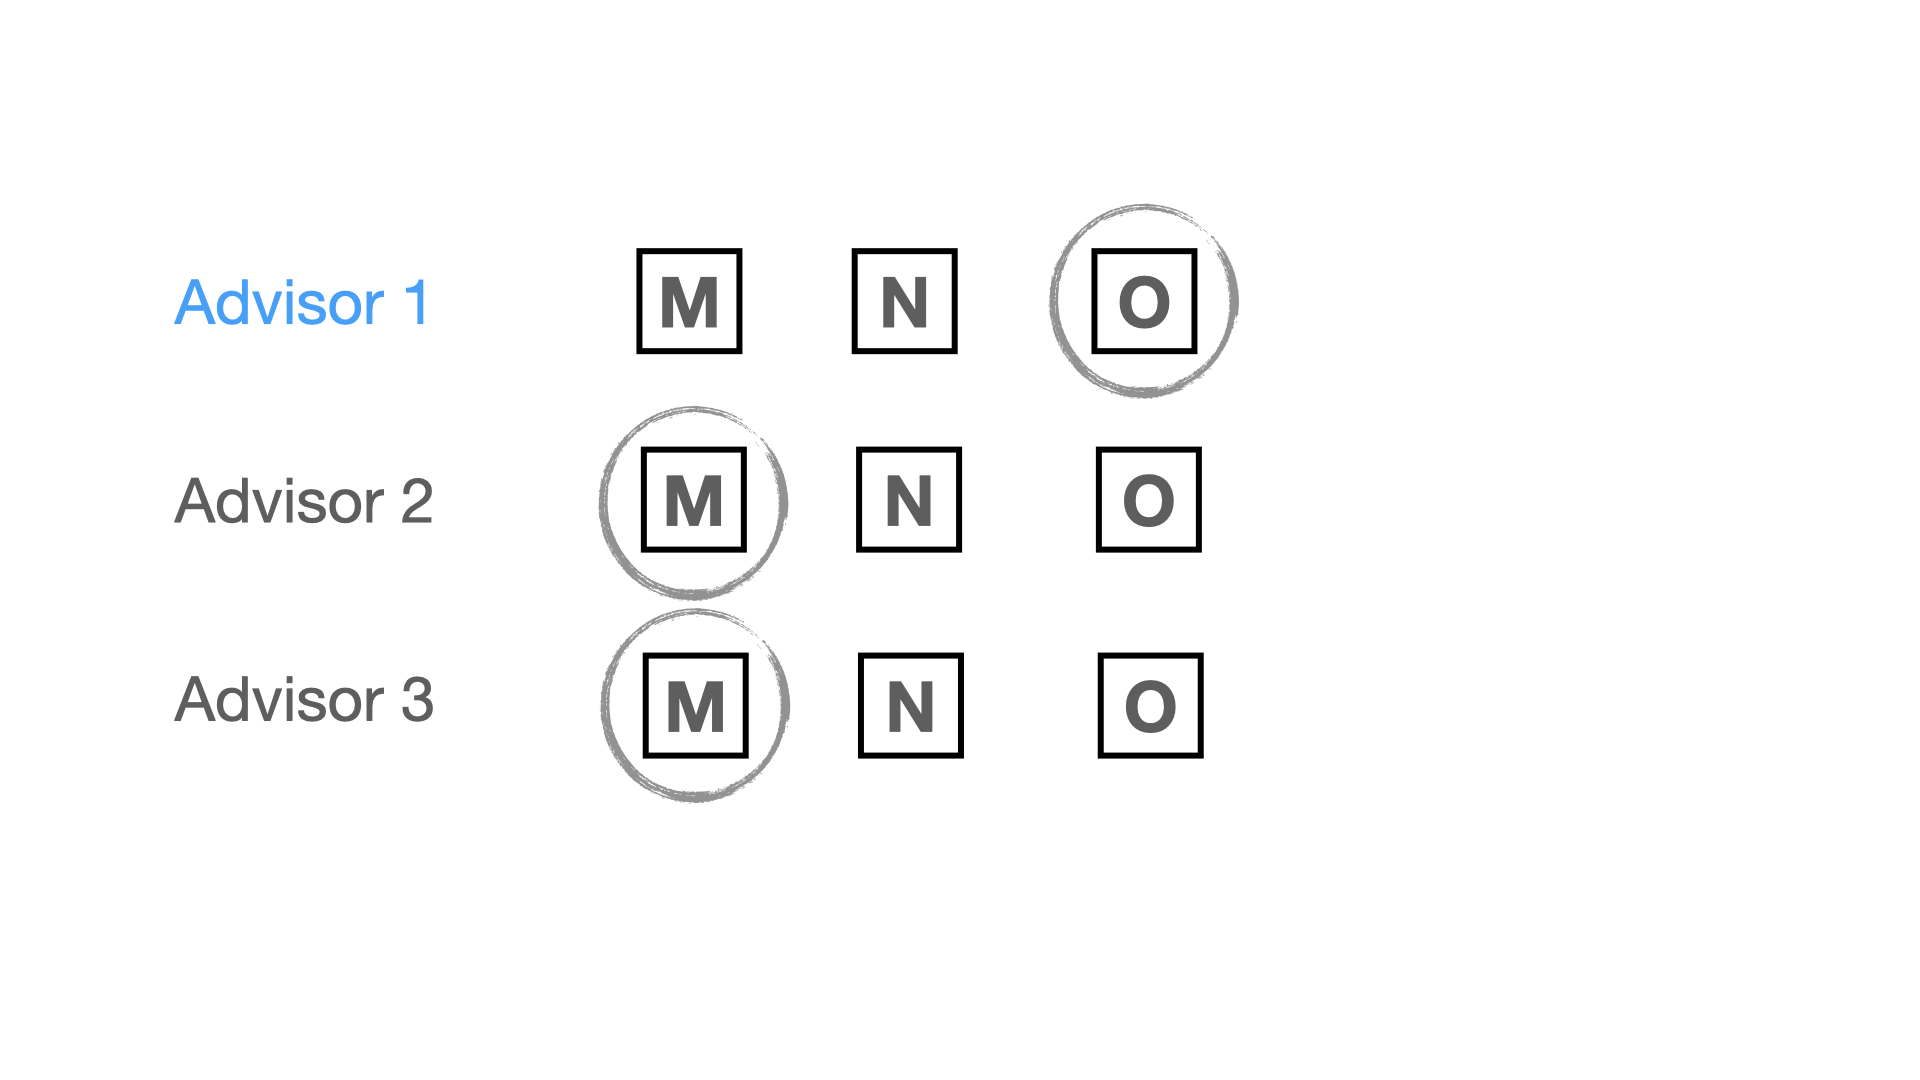
\includegraphics[width=0.6\textwidth,height=\textheight]{Experiment_4/figures/stimuli/opp_majority_b.png} \\
dissensus (1) & 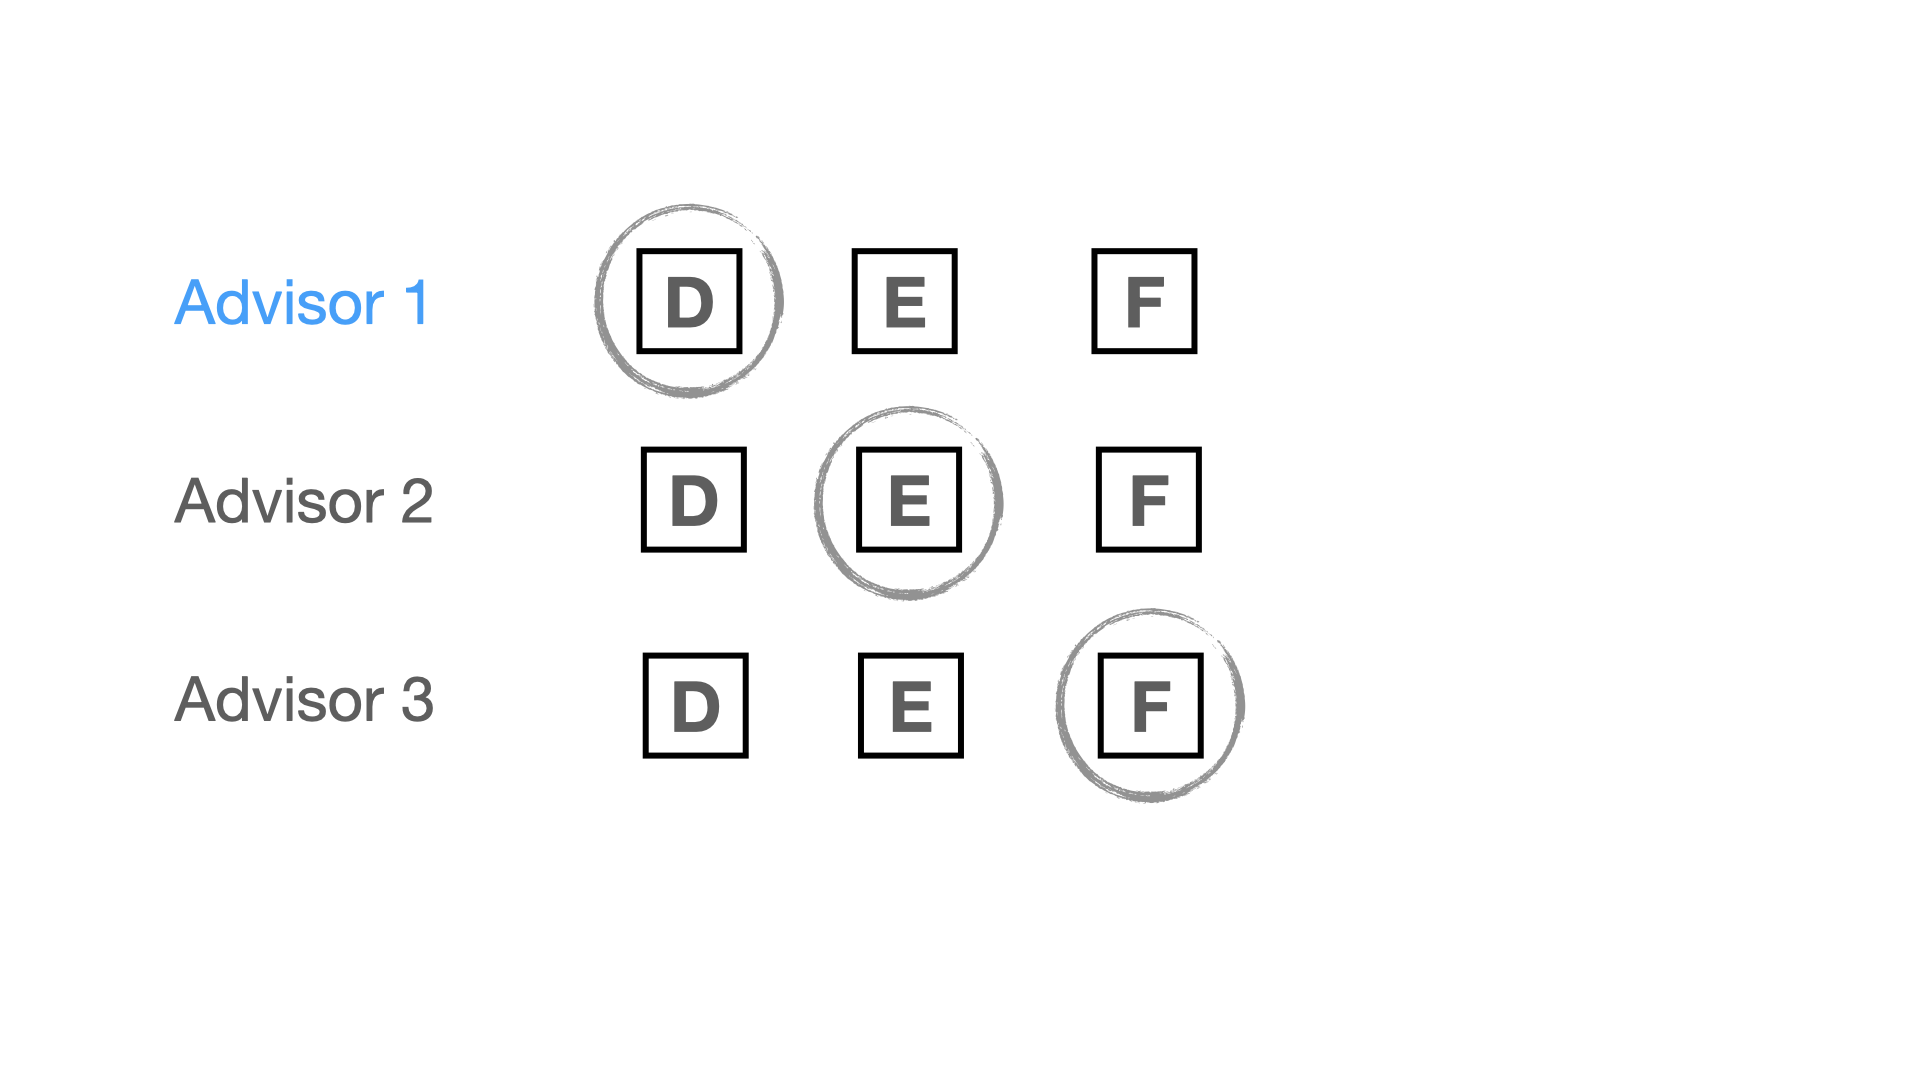
\includegraphics[width=0.6\textwidth,height=\textheight]{Experiment_4/figures/stimuli/divergence_a.png} & 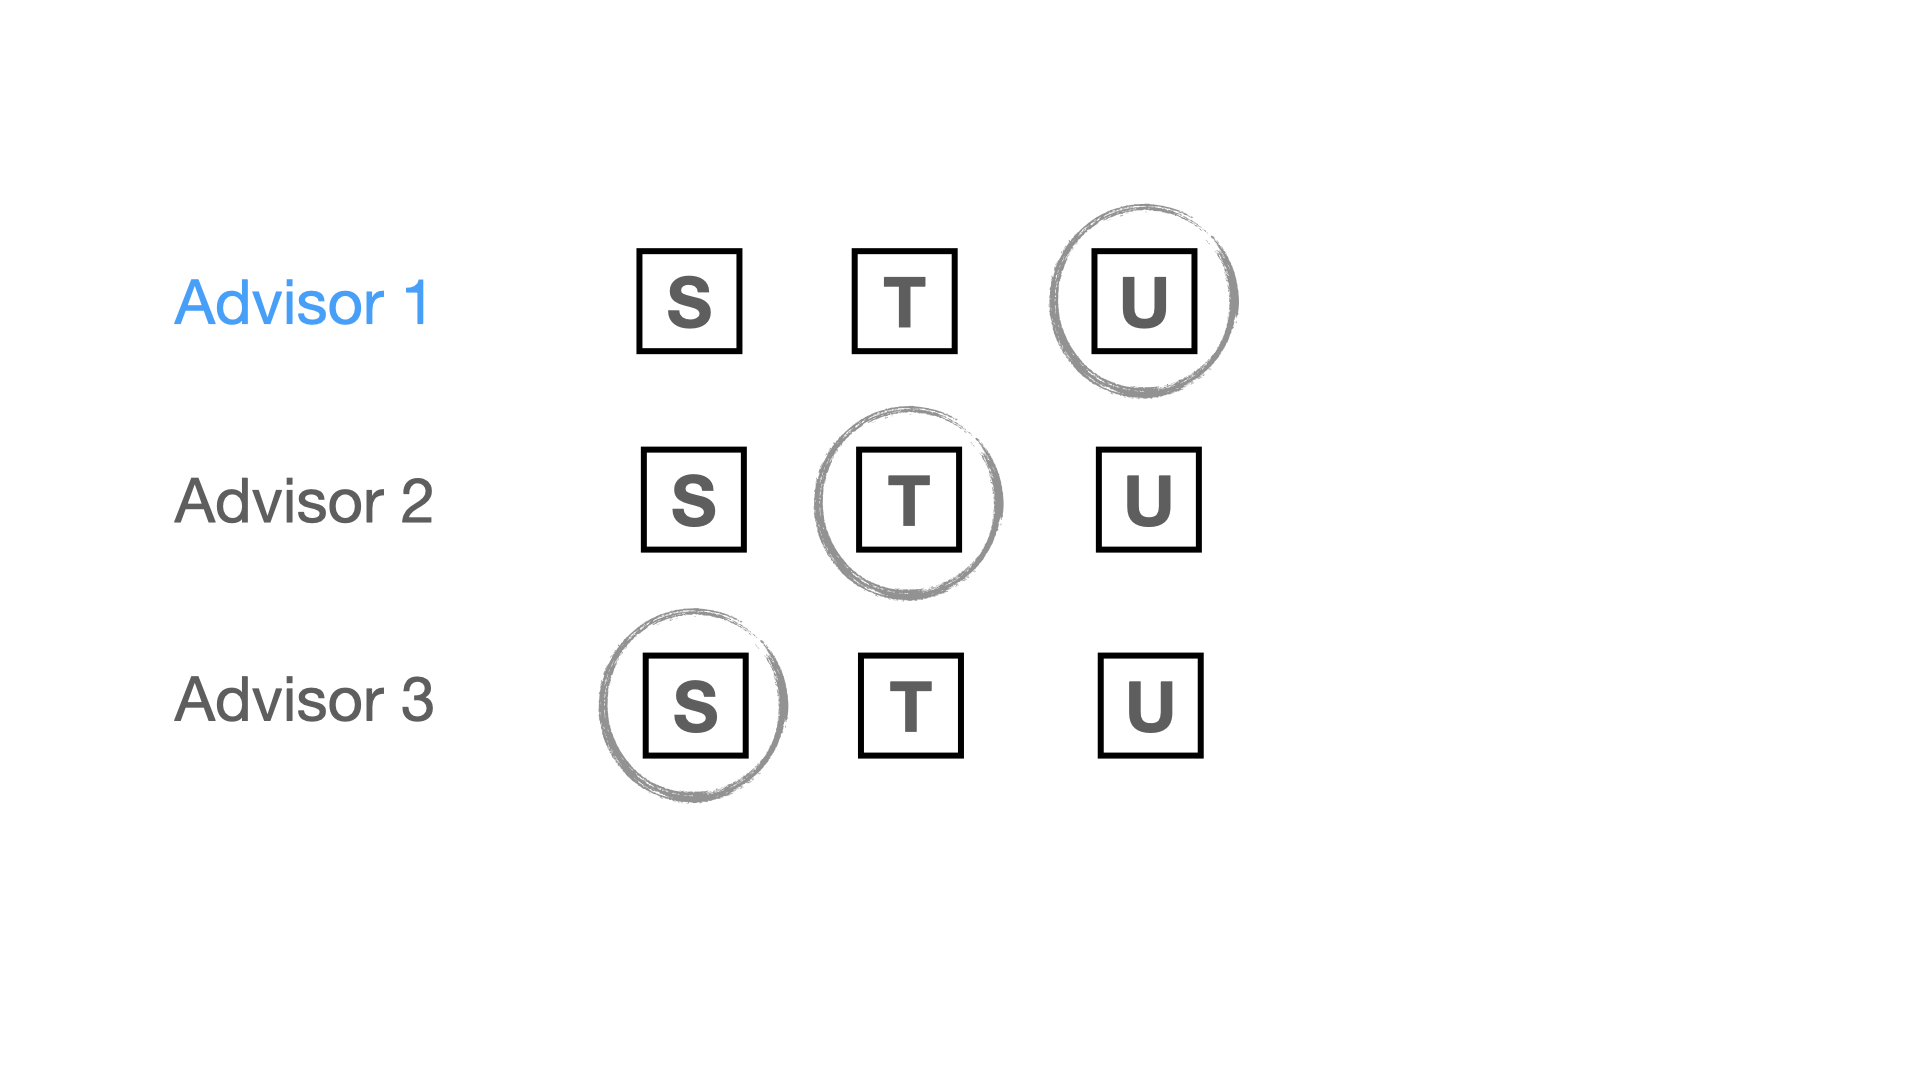
\includegraphics[width=0.6\textwidth,height=\textheight]{Experiment_4/figures/stimuli/divergence_b.png} \\
majority (2) & 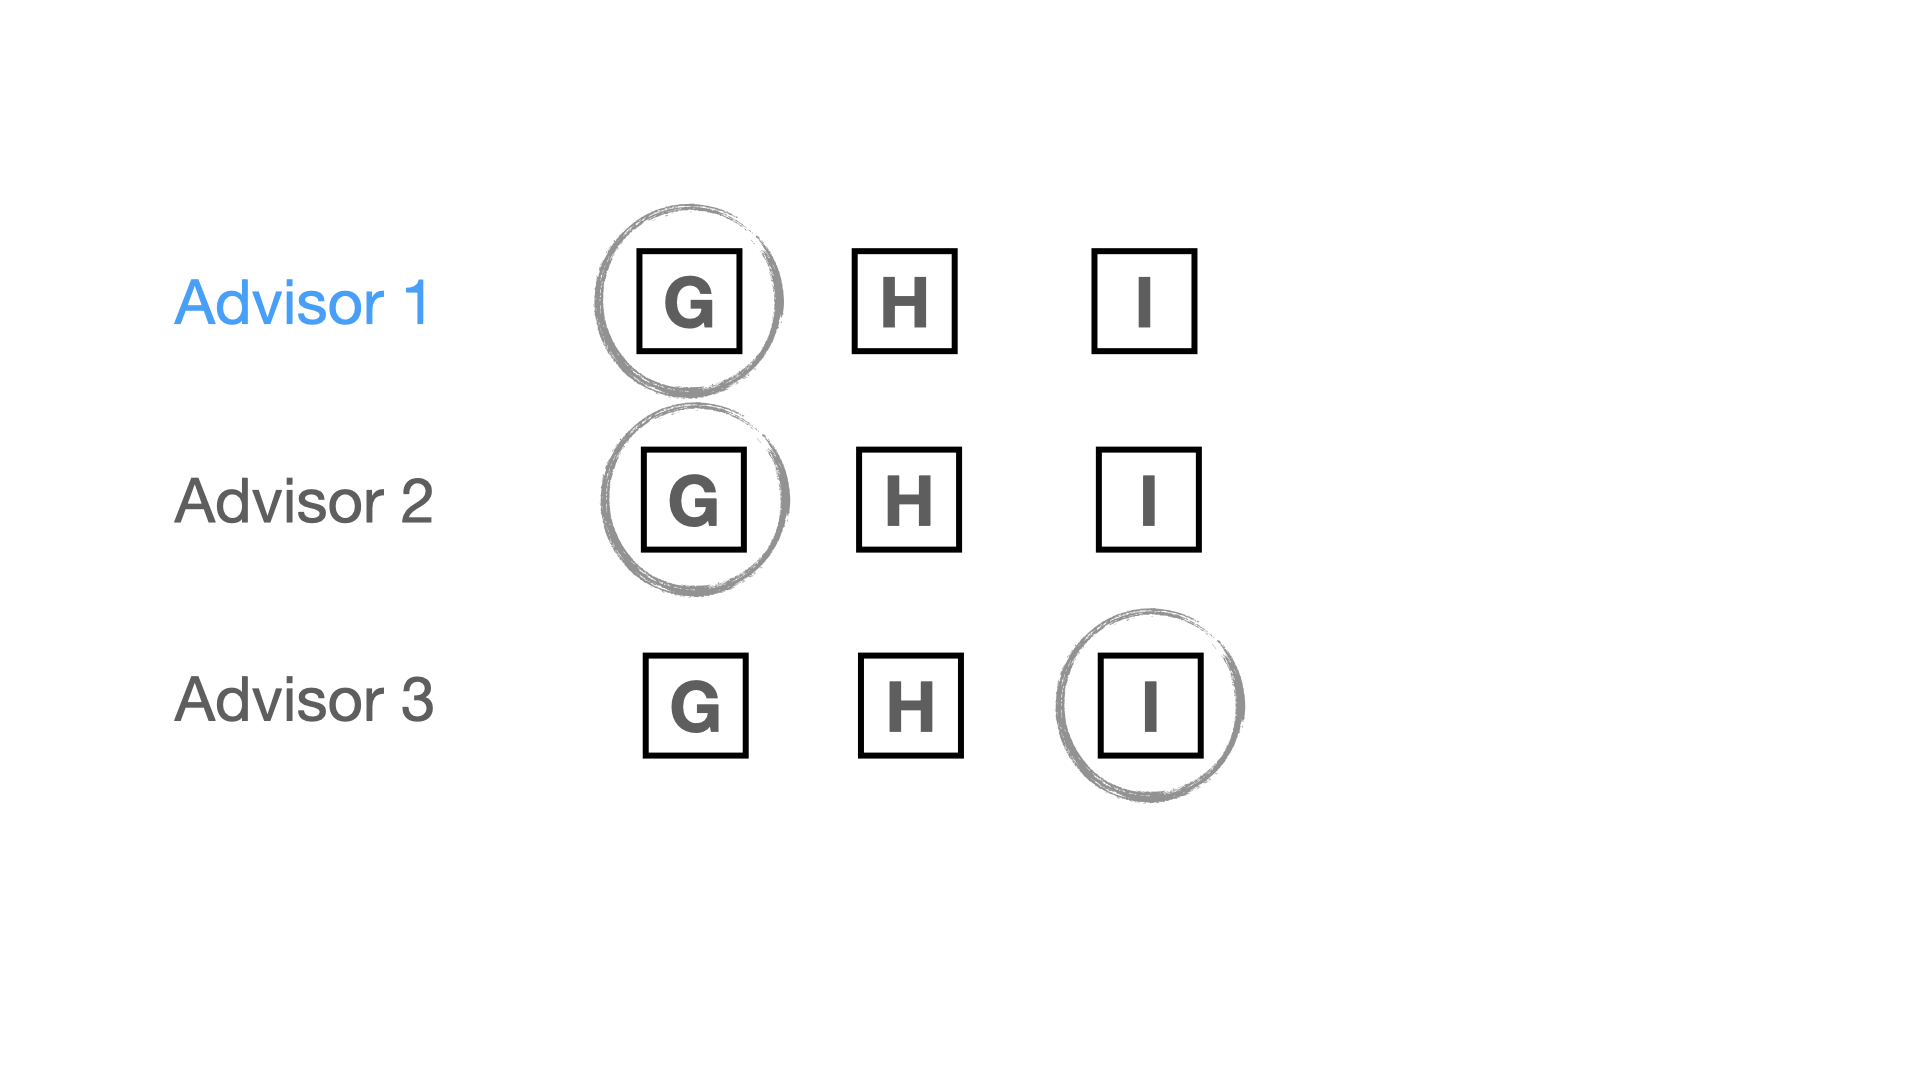
\includegraphics[width=0.6\textwidth,height=\textheight]{Experiment_4/figures/stimuli/majority_a.png} & 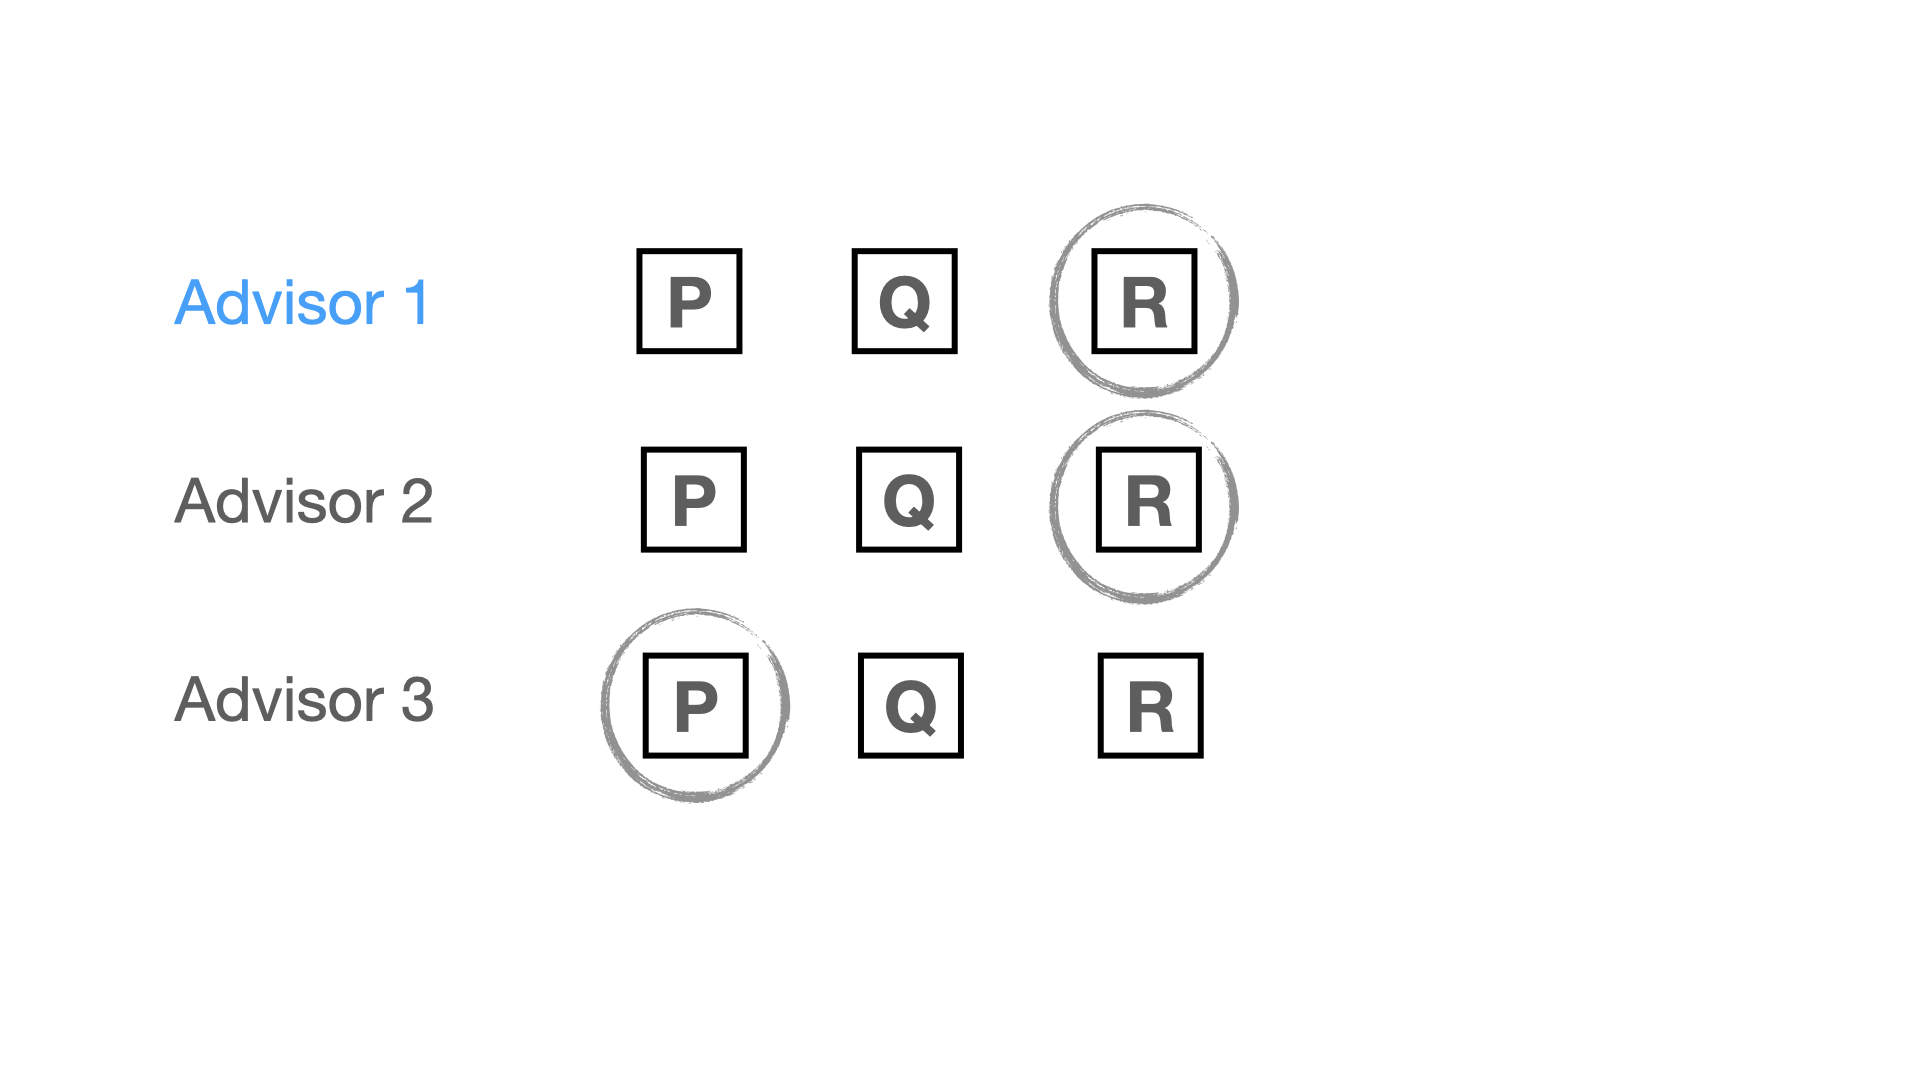
\includegraphics[width=0.6\textwidth,height=\textheight]{Experiment_4/figures/stimuli/majority_b.png} \\
consensus (3) & 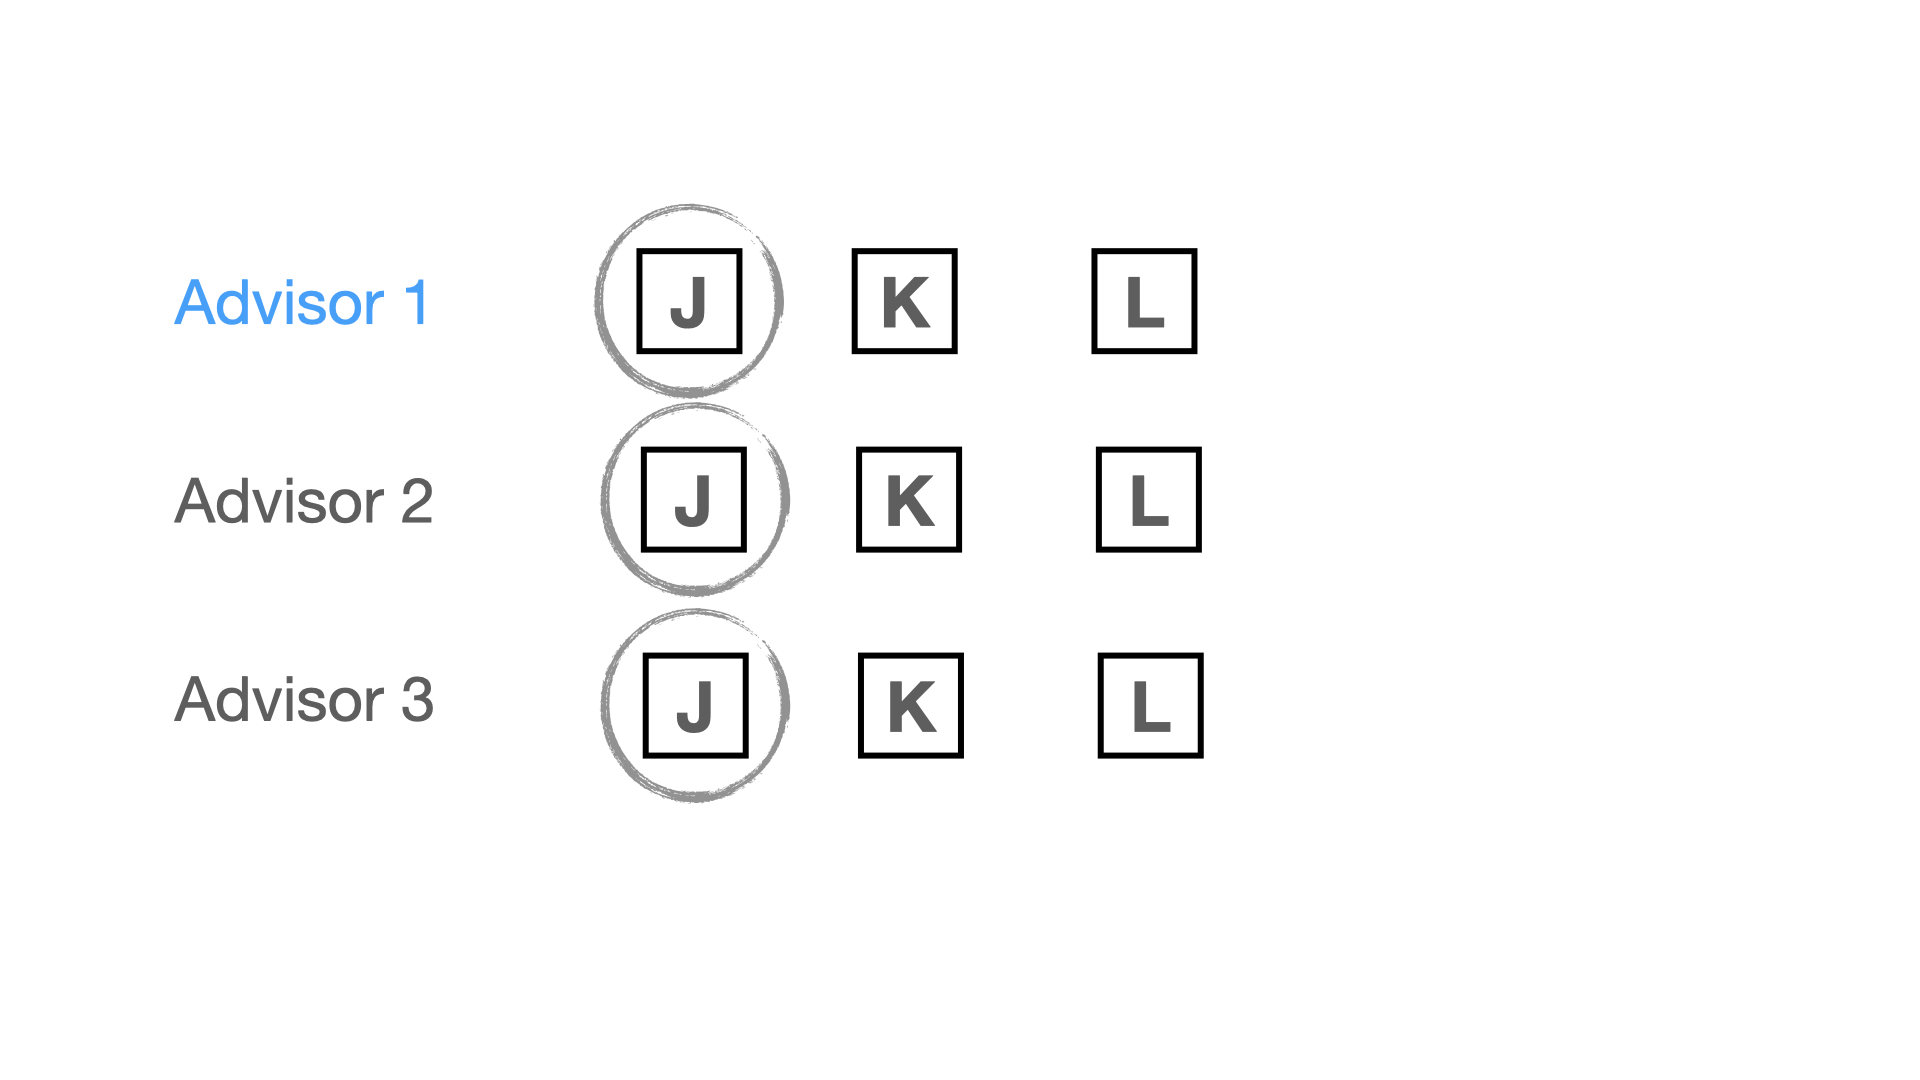
\includegraphics[width=0.6\textwidth,height=\textheight]{Experiment_4/figures/stimuli/consensus_a.png} & 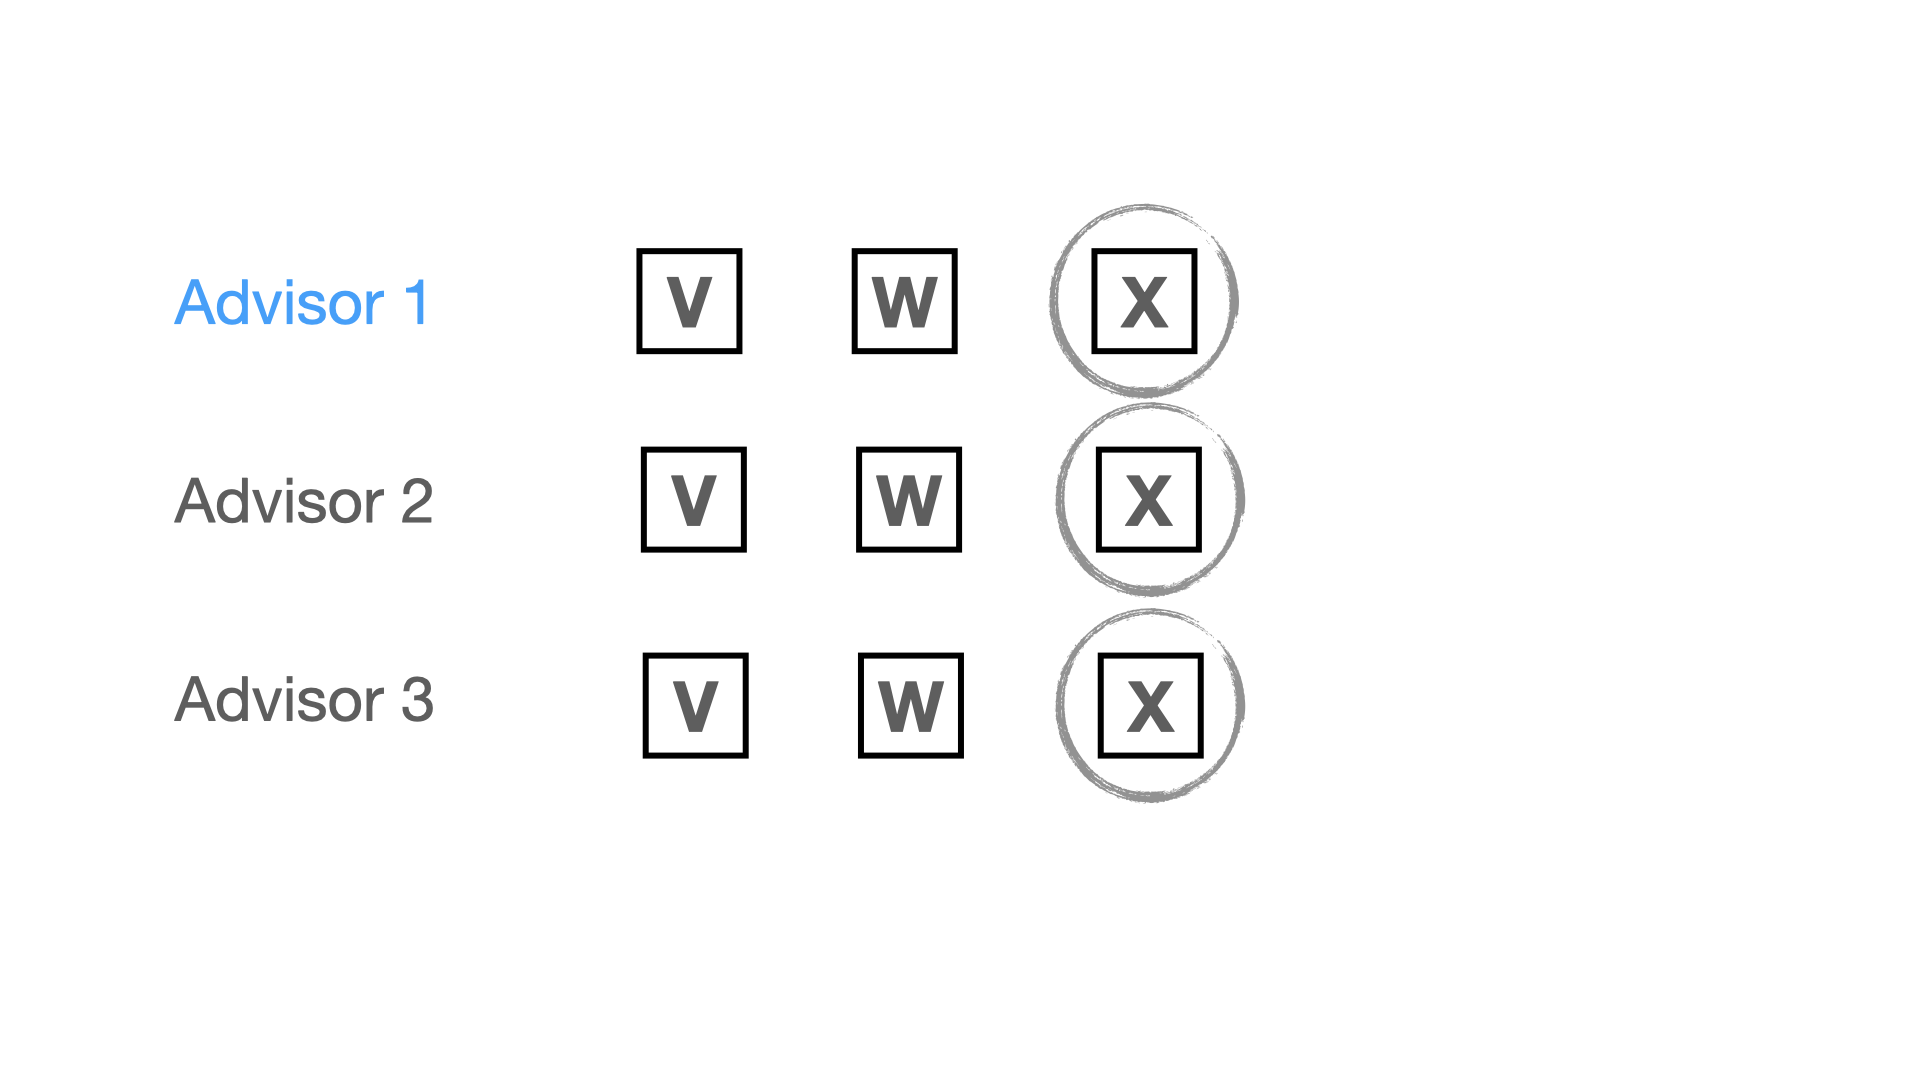
\includegraphics[width=0.6\textwidth,height=\textheight]{Experiment_4/figures/stimuli/consensus_b.png} \\
\end{longtable}

\subsection{Results}\label{results-3}

Table \ref{tab:exp4-table} contains descriptive results and Figure \ref{fig:exp4-plot} visualizes the results.

\begin{table}[tbp]

\begin{center}
\begin{threeparttable}

\caption{\label{tab:exp4-table}}

\begin{tabular}{lll}
\toprule
Convergence & \multicolumn{1}{c}{Accuracy} & \multicolumn{1}{c}{Competence}\\
\midrule
minority (0) & 33.13 (sd = 18.267) & 3.49 (sd = 1.156)\\
divergence (1) & 38.525 (sd = 13.708) & 3.93 (sd = 0.726)\\
majority (2) & 64.065 (sd = 13.86) & 4.88 (sd = 0.713)\\
consensus (3) & 80.745 (sd = 18.633) & 5.45 (sd = 0.981)\\
\bottomrule
\end{tabular}

\end{threeparttable}
\end{center}

\end{table}



\begin{figure}
\centering
\includegraphics{output/figures/exp4-plot.pdf}
\caption{\label{fig:exp4-plot}Results of Experiment 4, showing the distributions of accuracy and competence by level of convergence.}
\end{figure}

\subsection{Comparison with simulation}\label{comparison-with-simulation}

We compared the accuracy and competence ratings of the participants to actual accuracy and competence values from simulated data. The data was generated using the model described in the main paper, and assuming a uniform competence distribution. Compared to this data generating model, participants underestimate the effect of convergence for both accuracy and competence, but more for accuracy. Table \ref{tab:model-vs-participant-table} compares the results of regressions on participant data and regressions on simulated data. Fig. \ref{fig:exp4-model} visualizes the results.

\begin{table}
\centering
\caption{\label{tab:model-vs-participant-table}Participants vs. Model (Exp. 4)}
\centering
\begin{tabular}[t]{lcccc}
\toprule
\multicolumn{1}{c}{ } & \multicolumn{2}{c}{Participants} & \multicolumn{2}{c}{Model} \\
\cmidrule(l{3pt}r{3pt}){2-3} \cmidrule(l{3pt}r{3pt}){4-5}
  & Accuracy & Competence & Accuracy  & Competence \\
\midrule
(Intercept) & 28.859*** & 3.413*** & 15.211*** & 3.233***\\
 & (1.702) & (0.098) & (0.221) & (0.008)\\
convergence & 16.838*** & 0.683*** & 28.471*** & 0.425***\\
 & (0.922) & (0.053) & (0.097) & (0.003)\\
SD (Intercept id) & 15.926 & 0.929 &  & \\
SD (convergence id) & 8.640 & 0.497 &  & \\
Cor (Intercept\textasciitilde{}convergence id) & -0.808 & -0.857 &  & \\
SD (Observations) & 10.159 & 0.553 &  & \\
\midrule
Num.Obs. & 800 & 800 & 333000 & 333000\\
R2 &  &  & 0.205 & 0.047\\
R2 Adj. &  &  & 0.205 & 0.047\\
R2 Marg. & 0.555 & 0.408 &  & \\
R2 Cond. & 0.839 & 0.786 &  & \\
AIC & 6402.6 & 1756.0 & 3301803.1 & 1051474.5\\
BIC & 6430.7 & 1784.1 & 3301835.2 & 1051506.7\\
ICC & 0.6 & 0.6 &  & \\
Log.Lik. &  &  & -1650898.534 & -525734.261\\
RMSE & 8.98 & 0.49 & 34.42 & 1.17\\
\bottomrule
\multicolumn{5}{l}{\rule{0pt}{1em}+ p $<$ 0.1, * p $<$ 0.05, ** p $<$ 0.01, *** p $<$ 0.001}\\
\end{tabular}
\end{table}



\begin{figure}
\centering
\includegraphics{output/figures/exp4-model.pdf}
\caption{\label{fig:exp4-model}Comparison of accuracy (top) and competence (bottom) ratings in participant data (left) to observed accuracy in simulated data (right), by level of convergence.}
\end{figure}

\clearpage

\section{Experiment 5}\label{exp5}

\FloatBarrier

\subsection{Attention check}\label{attention-check-4}

Imagine you are playing video games with a friend and at some point your friend says: ``I don't want to play this game anymore! To make sure that you read the instructions, please write the three following words''I pay attention'' in the box below. I really dislike this game, it's the most overrated game ever.''

Do you agree with your friend? (Yes/No)

\subsection{Results}\label{results-4}

Table \ref{tab:exp5-table} contains descriptive results.

\begin{table}
\centering
\caption{\label{tab:exp5-table}}
\centering
\resizebox{\ifdim\width>\linewidth\linewidth\else\width\fi}{!}{
\begin{tabular}[t]{lllll}
\toprule
\multicolumn{1}{c}{} & \multicolumn{2}{c}{Accuracy} & \multicolumn{2}{c}{Competence} \\
\cmidrule(l{3pt}r{3pt}){2-3} \cmidrule(l{3pt}r{3pt}){4-5}
  & Conflict of interest & Independent & Conflict of interest & Independent\\
\midrule
minority (0) & 39.733 (sd = 20.238) & 36.46 (sd = 16.793) & 3.802 (sd = 1.146) & 3.606 (sd = 1.006)\\
divergence (1) & 41.52 (sd = 13.344) & 42.51 (sd = 13.6) & 4.005 (sd = 0.878) & 4.045 (sd = 0.839)\\
majority (2) & 55.416 (sd = 16.637) & 59.515 (sd = 14.575) & 4.495 (sd = 0.921) & 4.737 (sd = 0.879)\\
consensus (3) & 66.198 (sd = 24.825) & 71.914 (sd = 23.457) & 4.96 (sd = 1.273) & 5.247 (sd = 1.264)\\
\bottomrule
\end{tabular}}
\end{table}

\clearpage

\section{Experiment 6}\label{exp6}

\subsection{Design}\label{design-6}

\FloatBarrier

The main focus of experiment 6 was on comparing 3-options conditions to 10-options conditions (see Table \ref{tab:stimuli-options}). Additionally, we varied between two versions of the 10-options conditions: one in which the range of the answers corresponded to the range of the three options condition (see Table \ref{tab:stimuli-10}), and another with increased range (see Table \ref{tab:stimuli-10-alt}).

\begin{longtable}[]{@{}
  >{\raggedright\arraybackslash}p{(\columnwidth - 2\tabcolsep) * \real{0.4965}}
  >{\raggedright\arraybackslash}p{(\columnwidth - 2\tabcolsep) * \real{0.5035}}@{}}
\caption{\label{tab:stimuli-options}Example of a consensus stimulus for the two `Number of option' conditions}\tabularnewline
\toprule\noalign{}
\begin{minipage}[b]{\linewidth}\raggedright
Number of options: 3
\end{minipage} & \begin{minipage}[b]{\linewidth}\raggedright
Number of options: 10
\end{minipage} \\
\midrule\noalign{}
\endfirsthead
\toprule\noalign{}
\begin{minipage}[b]{\linewidth}\raggedright
Number of options: 3
\end{minipage} & \begin{minipage}[b]{\linewidth}\raggedright
Number of options: 10
\end{minipage} \\
\midrule\noalign{}
\endhead
\bottomrule\noalign{}
\endlastfoot
\includegraphics[width=0.4\textwidth,height=\textheight]{stimuli/Experiment_6/stimuli_Exp6/consensus_3_a.png} & \includegraphics[width=0.4\textwidth,height=\textheight]{stimuli/Experiment_6/stimuli_Exp6/consensus_10_a.png} \\
\end{longtable}

\subsection{Attention check}\label{attention-check-5}

Imagine you are playing video games with a friend and at some point your friend says: ``I don't want to play this game anymore! To make sure that you read the instructions, please write the three following words''I pay attention'' in the box below. I really dislike this game, it's the most overrated game ever.''

Do you agree with your friend? (Yes/No)

\subsection{Stimuli}\label{stimuli-3}

\begin{longtable}[]{@{}
  >{\centering\arraybackslash}p{(\columnwidth - 4\tabcolsep) * \real{0.0993}}
  >{\centering\arraybackslash}p{(\columnwidth - 4\tabcolsep) * \real{0.4503}}
  >{\centering\arraybackslash}p{(\columnwidth - 4\tabcolsep) * \real{0.4503}}@{}}
\caption{\label{tab:stimuli-10}Stimuli for 10 options condition by levels of convergence}\tabularnewline
\toprule\noalign{}
\begin{minipage}[b]{\linewidth}\centering
Level
\end{minipage} & \begin{minipage}[b]{\linewidth}\centering
Version a)
\end{minipage} & \begin{minipage}[b]{\linewidth}\centering
Version b)
\end{minipage} \\
\midrule\noalign{}
\endfirsthead
\toprule\noalign{}
\begin{minipage}[b]{\linewidth}\centering
Level
\end{minipage} & \begin{minipage}[b]{\linewidth}\centering
Version a)
\end{minipage} & \begin{minipage}[b]{\linewidth}\centering
Version b)
\end{minipage} \\
\midrule\noalign{}
\endhead
\bottomrule\noalign{}
\endlastfoot
minority (0) & \includegraphics[width=0.4\textwidth,height=\textheight]{Experiment_6/figures/stimuli/minority_10_a.png} & \includegraphics[width=0.4\textwidth,height=\textheight]{Experiment_6/figures/stimuli/minority_10_b.png} \\
dissensus (1) & \includegraphics[width=0.4\textwidth,height=\textheight]{Experiment_6/figures/stimuli/divergence_10_a.png} & \includegraphics[width=0.4\textwidth,height=\textheight]{Experiment_6/figures/stimuli/divergence_10_b.png} \\
majority (2) & \includegraphics[width=0.4\textwidth,height=\textheight]{Experiment_6/figures/stimuli/majority_10_a.png} & \includegraphics[width=0.4\textwidth,height=\textheight]{Experiment_6/figures/stimuli/majority_10_b.png} \\
consensus (3) & \includegraphics[width=0.4\textwidth,height=\textheight]{Experiment_6/figures/stimuli/consensus_10_a.png} & \includegraphics[width=0.4\textwidth,height=\textheight]{Experiment_6/figures/stimuli/consensus_10_b.png} \\
\end{longtable}

\begin{longtable}[]{@{}
  >{\centering\arraybackslash}p{(\columnwidth - 4\tabcolsep) * \real{0.0943}}
  >{\centering\arraybackslash}p{(\columnwidth - 4\tabcolsep) * \real{0.4528}}
  >{\centering\arraybackslash}p{(\columnwidth - 4\tabcolsep) * \real{0.4528}}@{}}
\caption{\label{tab:stimuli-10-alt}Alternative stimuli for 10 options condition by levels of convergence}\tabularnewline
\toprule\noalign{}
\begin{minipage}[b]{\linewidth}\centering
Level
\end{minipage} & \begin{minipage}[b]{\linewidth}\centering
Version a)
\end{minipage} & \begin{minipage}[b]{\linewidth}\centering
Version b)
\end{minipage} \\
\midrule\noalign{}
\endfirsthead
\toprule\noalign{}
\begin{minipage}[b]{\linewidth}\centering
Level
\end{minipage} & \begin{minipage}[b]{\linewidth}\centering
Version a)
\end{minipage} & \begin{minipage}[b]{\linewidth}\centering
Version b)
\end{minipage} \\
\midrule\noalign{}
\endhead
\bottomrule\noalign{}
\endlastfoot
minority (0) & \includegraphics[width=0.4\textwidth,height=\textheight]{Experiment_6/figures/stimuli/minority_10_a_alt.png} & \includegraphics[width=0.4\textwidth,height=\textheight]{Experiment_6/figures/stimuli/minority_10_b_alt.png} \\
dissensus (1) & \includegraphics[width=0.4\textwidth,height=\textheight]{Experiment_6/figures/stimuli/divergence_10_a_alt.png} & \includegraphics[width=0.4\textwidth,height=\textheight]{Experiment_6/figures/stimuli/divergence_10_b_alt.png} \\
majority (2) & \includegraphics[width=0.4\textwidth,height=\textheight]{Experiment_6/figures/stimuli/majority_10_a_alt.png} & \includegraphics[width=0.4\textwidth,height=\textheight]{Experiment_6/figures/stimuli/majority_10_b_alt.png} \\
consensus (3) & \includegraphics[width=0.4\textwidth,height=\textheight]{Experiment_6/figures/stimuli/consensus_10_a_alt.png} & \includegraphics[width=0.4\textwidth,height=\textheight]{Experiment_6/figures/stimuli/consensus_10_b_alt.png} \\
\end{longtable}

\subsection{Results}\label{results-5}

Figure \ref{fig:exp5-plot} visualizes the results and table \ref{tab:exp5-table} contains descriptive results.

\begin{table}
\centering\centering
\caption{\label{tab:exp6-table}}
\centering
\resizebox{\ifdim\width>\linewidth\linewidth\else\width\fi}{!}{
\begin{tabular}[t]{lllll}
\toprule
\multicolumn{1}{c}{} & \multicolumn{2}{c}{Accuracy} & \multicolumn{2}{c}{Competence} \\
\cmidrule(l{3pt}r{3pt}){2-3} \cmidrule(l{3pt}r{3pt}){4-5}
  & 10 options & 3 options & 10 options & 3 options\\
\midrule
minority (0) & 32.333 (sd = 22.987) & 35.703 (sd = 20.829) & 3.61 (sd = 1.245) & 3.574 (sd = 1.227)\\
divergence (1) & 37.287 (sd = 19.569) & 40.861 (sd = 18.759) & 4.067 (sd = 0.831) & 4.01 (sd = 0.881)\\
majority (2) & 63.69 (sd = 21.826) & 64.301 (sd = 17.355) & 4.957 (sd = 0.885) & 4.834 (sd = 0.881)\\
consensus (3) & 79.967 (sd = 24.15) & 80.152 (sd = 20.774) & 5.647 (sd = 1.035) & 5.466 (sd = 1.051)\\
\bottomrule
\end{tabular}}
\end{table}



\begin{figure}
\centering
\includegraphics{output/figures/exp6-plot.pdf}
\caption{\label{fig:exp6-plot}Interaction of convergence and informational dependency.}
\end{figure}

\subsection{Comparison with simulation}\label{comparison-with-simulation-1}

Since we didn't find a difference between three and ten choice option scenarios in the participant data, we wanted to have a normative point of reference of what should have been the expected difference, given our model. We therefor compared participant ratings to observed values from simulated data. The data was generated using the model described in the main paper, and assuming a uniform competence distribution. Compared to this data generating model, participants considerably underestimated how the number of choice options alters the effect of convergence for both accuracy and competence. Table \ref{tab:model-vs-participant-table} compares the results of regressions on participant data and regressions on simulated data. Fig. \ref{fig:exp6-model} visualizes the results.

\begin{table}
\centering
\caption{\label{tab:unnamed-chunk-98}Participants vs. Model (Exp. 6)}
\centering
\begin{tabular}[t]{lcccc}
\toprule
\multicolumn{1}{c}{ } & \multicolumn{2}{c}{Participants} & \multicolumn{2}{c}{Model} \\
\cmidrule(l{3pt}r{3pt}){2-3} \cmidrule(l{3pt}r{3pt}){4-5}
  & Accuracy & Competence & Accuracy  & Competence \\
\midrule
(Intercept) & 29.830*** & 3.508*** & 11.407*** & 3.189***\\
 & (1.197) & (0.063) & (0.220) & (0.009)\\
convergence & 16.305*** & 0.675*** & 31.596*** & 0.526***\\
 & (0.600) & (0.032) & (0.130) & (0.005)\\
number\_options\_effect\_code & -3.812 & 0.024 & -13.794*** & -0.207***\\
 & (2.394) & (0.126) & (0.439) & (0.018)\\
convergence × number\_options\_effect\_code & 1.252 & 0.050 & 8.498*** & 0.251***\\
 & (1.200) & (0.065) & (0.260) & (0.011)\\
SD (Intercept id) & 19.383 & 1.031 &  & \\
SD (convergence id) & 9.625 & 0.527 &  & \\
Cor (Intercept\textasciitilde{}convergence id) & -0.699 & -0.829 &  & \\
SD (Observations) & 12.103 & 0.598 &  & \\
\midrule
Num.Obs. & 2384 & 2384 & 51003 & 51003\\
R2 &  &  & 0.539 & 0.165\\
R2 Adj. &  &  & 0.539 & 0.165\\
R2 Marg. & 0.423 & 0.355 &  & \\
R2 Cond. & 0.814 & 0.779 &  & \\
AIC & 19980.3 & 5624.5 & 497742.9 & 170192.2\\
BIC & 20026.5 & 5670.7 & 497787.1 & 170236.4\\
ICC & 0.7 & 0.7 &  & \\
Log.Lik. &  &  & -248866.472 & -85091.109\\
RMSE & 10.67 & 0.53 & 31.83 & 1.28\\
\bottomrule
\multicolumn{5}{l}{\rule{0pt}{1em}+ p $<$ 0.1, * p $<$ 0.05, ** p $<$ 0.01, *** p $<$ 0.001}\\
\end{tabular}
\end{table}



\begin{figure}
\centering
\includegraphics{output/figures/exp6-model.pdf}
\caption{\label{fig:exp6-model}Comparison of accuracy (top) and competence (bottom) ratings in participant data (left) to observations in simulated data (right), by level of convergence.}
\end{figure}


\end{document}
